% Version 5.0, 2 January 2020

% This tex file can be compiled with
% tectonic templateV5.tex
% https://tectonic-typesetting.github.io
%
% Or simply with the Overleaf latexmkrc configuration: (included in the repo)
% https://www.overleaf.com/learn/how-to/How_does_Overleaf_compile_my_project%3F
%
% A latexindent.yml config file is also included for easier and more consistent
% formatting.

% %%%%%%%%%%%%%%%%%%%%%%%%%%%%%%%%%%%%%%%%%%%%%%%%%%%%%%%%%%%%%%%%%%%%%%%%%%%%%%%%%%%%%%
% TemplateV5.tex -- LaTeX-based template for submissions to the American Meteorological
% Society
% %%%%%%%%%%%%%%%%%%%%%%%%%%%%%%%%%%%%%%%%%%%%%%%%%%%%%%%%%%%%%%%%%%%%%%%%%%%%%%%%%%%%%%
% PREAMBLE
% %%%%%%%%%%%%%%%%%%%%%%%%%%%%%%%%%%%%%%%%%%%%%%%%%%%%%%%%%%%%%%%%%%%%%%%%%%%%%%%%%%%%%%

% Start with one of the following: DOUBLE-SPACED VERSION FOR SUBMISSION TO THE AMS
% \documentclass{ametsocV5}

% TWO-COLUMN JOURNAL PAGE LAYOUT---FOR AUTHOR USE ONLY
\documentclass[twocol]{ametsocV5}

% Enter packages here. If too many math alphabets are used, remove unnecessary packages
% or define hmmax and bmmax as necessary.
%\newcommand{\hmmax}{0}
%\newcommand{\bmmax}{0}
\usepackage{amsmath,amsfonts,amssymb,bm}
\usepackage{mathptmx}% {times}
\usepackage{newtxtext}
\usepackage{newtxmath}
\usepackage[version=4]{mhchem}
\usepackage[acronym]{glossaries}
\usepackage[printonlyused,withpage]{acronym}
\usepackage{cleveref}
\usepackage[separate-uncertainty=true]{siunitx}
\usepackage{listings}
% \usepackage{hyperref}

\makeglossaries{}
\newacronym{agcm}{AGCM}{Atmosphere General Circulation Model}
\newacronym{aodm}{AODVISstdn}{``stratospheric aerosol optical depth 550 nm day night''}
\newacronym{aod}{AOD}{(stratospheric) aerosol optical depth}
\newacronym{aogcm}{AOGCM}{Atmosphere-Ocean General Circulation Model}
\newacronym{c2wmp}{C2W\(-\)}{CESM2(WACCM6) intermediate strength}
\newacronym{c2wm}{C2W\(\downarrow\)}{CESM2(WACCM6) small strength}
\newacronym{c2wsn}{C2WN\(\uparrow\)}{CESM2(WACCM6) large strength, high northern latitude}
\newacronym{c2ws}{C2W\(\uparrow\)}{CESM2(WACCM6) large strength}
\newacronym{c2w}{C2W}{CESM2(WACCM6) tropical}
\newacronym{cam5}{CAM5}{Community Atmosphere Model Version 5}
\newacronym{cam6}{CAM6}{Community Atmosphere Model Version 6}
\newacronym{cesm1}{CESM1}{Community Earth System Model Version 1}
\newacronym{cesm2}{CESM2}{Community Earth System Model Version 2}
\newacronym{cesm}{CESM}{Community Earth System Model}
\newacronym{cice}{CICE5}{CICE Version 5.1.2}
\newacronym{cime}{CIME}{Common Infrastructure for Modelling the Earth}
\newacronym{cism}{CISM2}{Community Ice Sheet Model Version 2.1}
\newacronym{clm}{CLM5}{Community Land Model Version 5}
\newacronym{ecs}{ECS}{equilibrium climate sensitivity}
\newacronym{erf}{ERF}{effective radiative forcing}
\newabbreviation{ob16}{OB16}{\citet{ottobliesner2016}}
\newacronym{esm}{ESM}{Earth System Model}
\newacronym{flnt}{FLNT}{``net longwave flux at the top of the model''}
\newacronym{fpp}{FPP}{Filtered Poisson Process}
\newacronym{fsnt}{FSNT}{``net solar flux at the top of the model''}
\newacronym{fsst}{\texttt{fSST1850}}{fixed sea-surface temperature}
\newacronym{irf}{IRF}{instantaneous radiative forcing}
\newacronym{lwcf}{LWCF}{``long wave cloud forcing''}
\newacronym{lw}{LW}{long wave}
\newacronym{mam3}{MAM3}{three mode version of the Modal Aerosol Module}
\newacronym{mam}{MAM}{Modal Aerosol Module}
\newacronym{marbl}{MARBL}{MARine Biogeochemistry Library}
\newacronym{ma}{MA}{middle atmosphere}
\newacronym{mosart}{MOSART}{MOdel for Scale Adaptive River Transport}
\newabbreviation{j05}{J05}{\citet{jones2005}}
\newabbreviation{g16}{G16}{\citet{gregory2016}}
\newabbreviation{m20}{M20}{\citet{marshall2020dataset}}
\newabbreviation{t10}{T10}{\citet{timmreck2010}}
\newabbreviation{n15}{N15}{\citet{niemeier2015}}
\newacronym{pop}{POP2}{Parallel Ocean Program Version 2}
\newacronym{qbo}{QBO}{quasi-biennial oscillation}
\newacronym{rf}{RF}{(effective) radiative forcing}
\newacronym{swcf}{SWCF}{``short wave cloud forcing''}
\newacronym{sw}{SW}{short wave}
\newacronym{tcrp}{TCRP}{transient climate response parameter}
\newacronym{toa}{TOA}{top-of-the-atmosphere}
\newacronym{trefht}{TREFHT}{``reference height temperature''}
\newacronym{waccm}{WACCM6}{Whole Atmosphere Community Climate Model Version 6}
\newacronym{ww3}{WW3}{Wave Watch Version 3}
\newacronym{ytt}{YTT}{Young Toba Tuff}


% Create some custom commands
\newcommand{\iso}[1][i]{{#1}njected \ce{SO2}}
% The content of the URL must be on its own line. The compiler works fine both ways, but
% the syntax highlighting is messed up by it.
\urldef\fssturl\url{
1850_CAM60%WCCM_CLM50%BGC-CROP_CICE%PRES_DOCN%DOM_MOSART_CISM2%NOEVOLVE_SWAV_TEST
}

% %%%%%%%%%%%%%%%%%%%%%%%%%%%%%%%%%%%%%%%%%%%%%%%%%%%%%%%%%%%%%%%%%%%%%%%%%%%%%%%%%%%%%%

% To be entered by author:
% May use \\ to break lines in title:
\title{
  Parameter Scan: Volcanic influence on climate across multiple magnitudes of injected
  \ce{SO2}
}

% Enter authors' names, as you see in this example: Use \correspondingauthor{} and
% \thanks{Current Affiliation:...} immediately following the appropriate author. Note
% that the \correspondingauthor{} command is NECESSARY. The \thanks{} commands are
% OPTIONAL.

\authors{
  Eirik Rolland Enger\correspondingauthor{Eirik Rolland Enger, eirik.r.enger@uit.no}
}

% Follow this form: \affiliation{American Meteorological Society, Boston, Massachusetts}
\affiliation{UiT The Arctic University of Norway, Tromsø, Norway}

% \affiliation{}

% If appropriate, add additional authors, different affiliations:
% In alphabetical order?
\extraauthor{Rune Graversen}\extraaffil{UiT The Arctic University of Norway, Tromsø, Norway}
\extraauthor{Martin Rypdal}\extraaffil{UiT The Arctic University of Norway, Tromsø, Norway}
\extraauthor{Audun Theodorsen}\extraaffil{UiT The Arctic University of Norway, Tromsø, Norway}
\extraauthor{Maria Rugenstein}\extraaffil{Colorado State University, Fort Collins, Colorado}

% %%%%%%%%%%%%%%%%%%%%%%%%%%%%%%%%%%%%%%%%%%%%%%%%%%%%%%%%%%%%%%%%%%%%%%%%%%%%%%%%%%%%%%
% ABSTRACT
%
% Enter your abstract here. Abstracts should not exceed 250 words in length!

\abstract{%
  Large eruptions to super-volcano sized eruptions are simulated in the \ac*{cesm2}
  climate model with the \ac*{waccm} atmosphere. Ensembles containing four members are
  simulated and the \ac*{aod} and \ac*{rf} from the eruptions are compared to determine
  how far the linear relationship between the two parameters hold. Simulating a
  Pinatubo-like eruption yields results consistent with several previous studies showing
  a slope of \(\sim \SI{-20}{\watt\metre^{-2}}\) per unit \ac*{aod}. Larger eruptions,
  however, show a clear time-after-eruption dependence, where the \ac*{rf} is relatively
  stronger than \ac*{aod} the first year after an eruption (higher cooling efficiency),
  while in the later phase their ratio is roughly constant for a given eruption
  strength, but where smaller eruptions have a larger ratio and as such are more
  efficient.
}

\begin{document}

% Necessary!
\maketitle

% %%%%%%%%%%%%%%%%%%%%%%%%%%%%%%%%%%%%%%%%%%%%%%%%%%%%%%%%%%%%%%%%%%%%%%%%%%%%%%%%%%%%%%
% SIGNIFICANCE STATEMENT/CAPSULE SUMMARY
% %%%%%%%%%%%%%%%%%%%%%%%%%%%%%%%%%%%%%%%%%%%%%%%%%%%%%%%%%%%%%%%%%%%%%%%%%%%%%%%%%%%%%%
%
% If you are including an optional significance statement for a journal article or a
% required capsule summary for BAMS (see
% www.ametsoc.org/ams/index.cfm/publications/authors/journal-and-bams-authors/formatting-and-manuscript-components
% for details), please apply the necessary command as shown below:
%
% \statement
% Significance statement here.
%
% \capsule
% Capsule summary here.

% %%%%%%%%%%%%%%%%%%%%%%%%%%%%%%%%%%%%%%%%%%%%%%%%%%%%%%%%%%%%%%%%%%%%%%%%%%%%%%%%%%%%%%
% MAIN BODY OF PAPER
% %%%%%%%%%%%%%%%%%%%%%%%%%%%%%%%%%%%%%%%%%%%%%%%%%%%%%%%%%%%%%%%%%%%%%%%%%%%%%%%%%%%%%%

% In all cases, if there is only one entry of this type within the higher level heading,
% use the star form:
%
% \section{Section title}
% \subsection*{subsection}
% text...
% \section{Section title}
%
% vs
%
% \section{Section title}
% \subsection{subsection one}
% text...
% \subsection{subsection two}
% \subsubsection{First tertiary heading}
% \paragraph{First quaternary heading}
% \section{Section title}

% NOTE: what to include in the paper, key questions.
% The paper should provide insight about what might happen if a large volcano erupted
% (order of magnitude or more than Mount Pinatubo). How does the atmosphere react, for
% example in the aerosol dynamics? (QBO, SO2/AOD/RF relationship.) It should also be
% about how volcanic simulations compare in magnitude and if there is time for more
% simulations, how model complexity (dynamic ocean against slab ocean) affect things.
% - How far does the linear relation between AOD and RF go? What phases does the
%   aerosols go though? (Perhaps the most promising avenue.)
% - How much does it matter how high in the atmosphere the initial SO2 is injected?
%   (Already is some literature on this, suggesting it is not much. Also some on
%   latitude dependence, which has a bigger influence.)
% - How does the climate response change based on the state of the climate: what if we
%   run a CO2 doubling or quadrupling simulation until close to equilibrium, and let the
%   volcanoes erupt then? (Lack the doubling scenario, and setting it up has resulted in
%   strange output that must be resolved. Could take a while.)

\section{Introduction and Motivation}

\paragraph*{Why volcanoes have been given attention}

During much of the past few thousand years, the Holocene, the natural climate
variability on Earth have been mostly forced by volcanic eruptions \citep{sigl2022}.
Despite the strong climate variability impact of volcanic eruptions, in particular up to
the current strong anthropogenic forcing of the climate,
% FIX: check that the Sigl part is correct and precise. (Comment from Rune.) I think so,
% at least if we make sure to specify that the simulations in mind are simulations over
% the Holocene.
few climate model experiments have included volcanic forcing when simulating climate
evolution during the Holocene \citep{sigl2022}, implying an exaggerated positive forcing
\citep{gregory2016}. Thus, even though the understanding of how volcanic eruptions force
the climate has been given much attention, questions for example related to aerosol
particle processes such as how they grow, which impacts their scattering efficiency and
possibly the \ac{aod} to \ac{rf} relationship is still unanswered
\citep[e.g.][]{robock2000,zanchettin2019,marshall2020,marshall2022}.
% FIX: what specifically is unanswered? Do I get into this in the later sections?

% NOTE: Section on similarities between CO2 and volcanic forcing. (feedback params
% references). Richardson is doing something that looks very similar to Gunther 2022.
% Mention that as well? (Similarity bw 0.5CO2 and volcanoes.)

\paragraph*{On similarities bw.\ \ce{CO2} and volcanoes (\ac{ecs})}

One avenue that has been given much attention is how forcing from volcanoes or
volcano-like forcings compares to the forcing that is due to increased \ce{CO2} levels.
\citet{boer2007,marvel2016,merlis2014,ollila2016,richardson2019,salvi2022,wigley2005}
all investigate the link, if any exists, between volcanic forcing and the climate
sensitivity to a doubling of \ce{CO2}, a much used metric for describing the severity of
global warming. This is motivated by the large uncertainty in estimates of the
sensitivity of the real climate system, and inferring climate sensitivity from for
example volcanoes have been used as an attempt to constrain the sensitivity
\citep{boer2007}.
% FIX: Explain how
Such a constraint rely on the assumption that volcanic forcing and \ce{CO2} forcing
produce correlated feedbacks \citep{pauling2023}. Among these, some have been running
simulations of the 1991 Mt.\ Pinatubo eruption \citep{merlis2014,ollila2016} or
historical volcano or volcano-like forcings \citep{boer2007,marvel2016,wigley2005},
while some investigate aerosol forcing in general \citep{richardson2019,salvi2022}. Many
earlier studies often assume that \ac{ecs} can be inferred from volcanoes
\citep{wigley2005} or suggest that it might be possible \citep{bender2010}, as long as
\ac{ecs} is constrained by \ac{erf} and not \ac{irf},
% FIX: explain what ERF and IRF are
which differ in that \ac{erf} account for rapid atmospheric adjustments while \ac{irf}
do not \citep{richardson2019}. Other studies suggest either that this is not possible
and that the sensitivity to volcanic forcing and \ce{CO2} doubling are different, or
that it is inaccurate since the precision at which climate simulations are run is not
high enough \citep{douglass2006,boer2007,salvi2022}. Even though \ac{erf} is a more
suited indicator of the temperature response to a forcing than \ac{irf}
\citep{marvel2016,richardson2019}, more recent studies conclude that \ac{ecs} cannot be
constrained from volcanoes \citep{pauling2023}.

\paragraph*{On aerosol evolution and atm.\ dynamics}

\ce{H2O}, \ce{N2} and \ce{CO2} are the most abundant gases emitted by volcanoes
\citep{robock2000}, but still, sulphur species like \ce{SO2} are the most influential
due to the already relatively large concentrations of the former gases in the
atmosphere. From \ce{SO2} \ce{H2SO4} is formed after reactions with \ce{OH} and \ce{H2O}
\citep{robock2000}. Sulphate acid, \ce{H2SO4}, produces the largest effect by
% FIX: mention the albedo effect
backscattering sunlight and thus increasing the planetary albedo and reducing the
\ac{rf} from the Sun, and since its formation from \ce{SO2} is happening over weeks
\citep{robock2000}, the peak \ac{rf} from the eruption has a slight delay from the onset
of the eruption. The duration of time that the \ce{H2SO4} aerosols stay in the
atmosphere depends on several factors, including the phase of the \ac{qbo}
\citep{pitari2016b}, the season of the year (determining to which hemisphere aerosols
are transported) \citep{toohey2011,toohey2019}, latitude \citep{marshall2019,
  toohey2019}, volcanic plume height \citep{marshall2019} and the aerosol size
\citep{marshall2019}. In the case of tropical eruptions, aerosols are typically
transported poleward in the stratosphere and back to mid-latitude troposphere within one
to two years \citep{robock2000}.
% TODO: mention that aerosols are washed out by droplets? This does not occur in the
% stratosphere

% Section on RF to AOD ratio

\paragraph*{On the comparison bw.\ \acs*{rf} and \acs*{aod}}

Previous studies on both Mt. Pinatubo alone \citep{mills2017,hansen2005} and volcanoes
in the instrumental era \citep{gregory2016} have been used to estimate the relationship
between the energy imbalance caused by volcanic eruptions and \ac{aod}.
\citet{myhre2013} use a formula for \ac{rf} that scales \ac{aod} by
\(\SI{-25}{\watt\metre^{-2}\mathrm{AOD}^{-1}}\) while values down to
\(\SI{-19.0(5)}{\watt\metre^{-2}\mathrm{AOD}^{-1}}\) \citep{gregory2016} and
\(\SI{-18.3(10)}{\watt\metre^{-2}\mathrm{AOD}^{-1}}\) \citep{mills2017} have been
reported more recently. Simulations done with synthetic volcanoes have also been used,
and in \citet{marshall2020} they obtain a scaling factor of
\(\SI{-20.5(2)}{\watt\metre^{-2}\mathrm{AOD}^{-1}}\) from simulating a total of \(82\)
volcanic eruptions with varying injection height and latitude, ranging from \(10\) to
\(\SI{100}{\tera\gram}\) of \iso{}.

A similar simulation setup, albeit with significant differences, was done by
\citet{niemeier2015}, where \(14\) different levels of injected sulphur ranging between
\(\SI{1}{\tera\gram(\ce{S})\mathrm{yr}^{-1}}\)
(\(\SI{2}{\tera\gram(\ce{SO2})\mathrm{yr}^{-1}}\)) and
\(\SI{100}{\tera\gram(\ce{S})\mathrm{yr}^{-1}}\)
(\(\SI{200}{\tera\gram(\ce{SO2})\mathrm{yr}^{-1}}\)) was simulated. These were
geoengineering simulations where sulphur would be continually injected, and the
simulations run until the sulphur level was in a steady state. From this, they found
that the \ac{rf} to injected rate ratio would follow an exponential and converge to a
value of \(\SI{-65}{\watt\metre^{-2}}\). While the results from the super-volcano
simulation by \citet{jones2005} indicate a much less steep gradient than the \(-18.3\)
to \(-25\) found in more recent literature, the peak \ac{rf} obtained in the
super-volcano simulation was \(\SI{-60}{\watt\metre^{-2}}\), which may suggest the
\citet{niemeier2015} results to be transferable to a volcanic eruption simulation
scenario.

\paragraph*{Aerosol optical depth vs.\ radiative forcing}

The aerosol evolution and lifetime in the stratosphere strongly influence the \ac{aod}
and the \ac{rf}, but not always in the same way. \citet{marshall2020} present results
showing higher efficiencies in years 2 and 3 after an eruption, compared to year 1,
explaining that this is due to the aerosols being concentrated more spatially in the
first year and more spread out in later years. This has the effect of increasing the
albedo per global mean \ac{aod} which in turn increases the \ac{rf} per \ac{aod}
\citep{marshall2020}. (Also, \ac{aod} to \ac{rf} depend on insulation, cloudiness and
surface albedo among others, which vary across eruptions
\citep{marshall2021,andersson2015}.)

% \citet{marshall2022} mention (in the graphic in their figure 1) that the \emph{role of
%   initial conditions} is a key outstanding question, especially if the \ce{CO2}
% doubling simulations work out, this could be a contribution to that.
% Also, when aerosols grow, they scatter radiation less efficiently and also fall down
% faster, so the temperature response should be comparatively weaker for increasing
% eruption magnitude (or the volcanic aerosols are less efficient). \emph{Clustering} and
% long term effects are mentioned in its own section (Multi-decadal impacts) along with
% the \emph{dependence of the current climate state}.

% \citet{marshall2019} does many similar things to what I have done, but do not focus on
% seasonal variability. This is however mentioned as one other direction to dig into, but
% is somewhat covered by \citet{marshall2020}. Assumes that there is an $e$-folding time,
% but notes that it does change, so they calculate an average time over a small range
% (from a month after the peak until reaching ten percent of the peak). They further note
% that the $e$-folding time is dependent on latitude mostly, but also on injected
% \ce{SO2}. Their eruptions all occur in July, but with the equivalent winter (January)
% eruptions covered by \citet{marshall2020}.

% In \citet{marshall2020}, they take the reconstructed \ac{aod} from
% \citet{toohey2017}, convert it to radiative forcing based on their conversions, and plot
% the corresponding temperature time series from each radiative forcing using a simple
% climate model. \emph{So, can we use this with the \ac{fpp} framework? (Noisy data?
%   Check this.)}
% TODO: check the data if it can be used for FPP.

% Perhaps focus on why there seems to be a loop in the \ac{aod} against
% \ac{rf} plots. Can also compare February-August means with May-November means.
% (\citet{marshall2021} discuss Tambora, but mention that it erupted in April, while their
% data consist of January and July eruptions.)

% \paragraph*{Motivation}
%
% From \citet{pauling2023}: what aspect of the climate system control the response to
% volcanic eruptions?
%
% From \citet{marshall2022}: However, uncertainties remain regarding the role of internal
% variability and the dependence on the current climate state. Also \citet{aubry2022} give
% a review on this very topic. They emphasise the urgency to accelerate research on
% climate-volcano impacts (a niche topic to date).

\section{Method}

\subsection{Model}

\begin{table*}
  \caption{\acl*{cesm2} model components}%
  \label{tab:cesm-components}
  \begin{center}
    \begin{tabular}[c]{ll}
      \multicolumn{1}{c}{\textbf{Component name}} &
      \multicolumn{1}{c}{\textbf{Reference}}                                              \\
      \acl*{cesm2}                                & \citet{danabasoglu2020}               \\
      \acl*{waccm}                                & \citet{gettleman2019}                 \\
      \acl*{pop}                                  & \citet{smith2010, danabasoglu2020}    \\
      \acl*{mosart}                               & \citet{li2013, danabasoglu2020}       \\
      \acl*{clm}                                  & \citet{lawrence2019, danabasoglu2020} \\
      \acl*{ww3}                                  & \citet{danabasoglu2020}               \\
      \acl*{cice}                                 & \citet{danabasoglu2020}               \\
      \acl*{cism}                                 & \citet{danabasoglu2020}               \\
      \acl*{cime}                                 & \citet{danabasoglu2020}
    \end{tabular}
  \end{center}
\end{table*}

We apply the \ac{cesm2} \citep{danabasoglu2020}, along with the \ac{waccm}
\citep{gettleman2019} and the fully dynamical ocean component \ac{pop} \citep{smith2010,
  danabasoglu2020}. The complete list of model components is found in
\cref{tab:cesm-components}. The model atmosphere was run at nominal \(\SI{2}{\degree}\)
resolution, with \(70\) vertical levels, in the \ac{ma} configuration.

The \ac{ma} version of \ac{waccm} uses the \ac{mam3} \citep{gettleman2019}. This is
implemented as a simplified and computationally efficient default setting in the
\ac{cam5} \citep{liu2016}, and is described in \citet{liu2012}. The \ac{mam3} was
developed from MAM7 (seven modes) by merging the primary carbon mode with the
accumulation mode, and assuming instantaneous internal mixing of primary carbonaceous
aerosols with secondary aerosols \citep{liu2016}. Specifically, the three modes are
Aitken, accumulation and coarse (MAM7 includes Aitken, accumulation, primary carbon,
fine dust and fine sea salt, coarse dust and coarse sea salt modes) \citep{liu2016}.
Instantaneous ageing of primary carbonaceous particles is assumed by emitting them in
the accumulation mode. There are \(15\) transported aerosol tracers in \ac{mam3}
\citep{liu2016}. \citet{marshall2019, marshall2020, marshall2021} used a code with seven
log-normal modes to simulate aerosol mass and number concentrations, but their model is
an \ac{agcm}, as opposed to the \ac{cesm2} which is an \ac{esm} or \ac{aogcm}.

Since dust efficiently absorbs water it is expected to be removed by wet deposition
similar to sea salt, which makes the course mode (mode 3, of which sea salt and soil
dust are both part of) quickly retain its background state below the tropopause
\citep{liu2012}. Similarly, fine dust and fine sea salt are both merged into the
accumulation mode (mode 2).

% NOTE: maybe Maria have an idea?
% \citet{liu2012} says the accumulation mode is roughly $90\%$ of the sulfate burden,
% which I don't really get from my figures. Hmm, need to look more into this.

\subsection{Simulation set up}

Simulations were created using a modified version of the file
\url{http://svn.code.sf.net/p/codescripts/code/trunk/ncl/emission/createVolcEruptV3.ncl},
% \href{http://svn.code.sf.net/p/codescripts/code/trunk/ncl/emission/createVolcEruptV3.ncl}{\texttt{createVolcEruptV3.ncl}}
via a Python project developed on GitHub at
\url{https://github.com/engeir/volcano-cooking}. The project is also available from the
Python package manager PyPI. The program creates volcanoes with a given \ce{SO2} amount
that is injected over six
hours\footnote{\url{http://svn.code.sf.net/p/codescripts/code/trunk/ncl/emission/createVolcEruptV3.ncl}}
at a given altitude, latitude and longitude. All volcanic \ce{SO2} files are created by
setting the eruption details in a .json file that is read to the
\texttt{volcano-cooking} CLI at a fixed version, making the experiment setup highly
reproducible.

We are using the \texttt{BWma1850} component
setup\footnote{\url{https://docs.cesm.ucar.edu/models/cesm2/config/2.1.0/compsets.html}}
to run the \ac{cesm2}, and an accompanying \ac{fsst}
% WARN: how should the fSST compset be referred to
simulation to obtain estimates of the \ac{rf}. The \ac{fsst} simulation used is not from
a standardised component setup as of \ac{cesm2} (v2.1.3), but is instead specified in
full.\footnote{\fssturl}
% as (\texttt{BWma1850} full name
% also shown for comparison)
% \begin{small}
%   \begin{verbatim}
% BWma1850 ->
%   1850_CAM60%WCCM_CLM50%BGC-CROP_CICE_
%   POP2%ECO%NDEP_MOSART_CISM2%NOEVOLVE_WW3
% fSST1850 ->
%   1850_CAM60%WCCM_CLM50%BGC-CROP_CICE%PRES_
%   DOCN%DOM_MOSART_CISM2%NOEVOLVE_SWAV_TEST
%   \end{verbatim}
% \end{small}
%
They differ in \texttt{CICE -> CICE\%PRES}, which is prescribed sea-ice,
\texttt{POP2\%ECO\%DEP -> DOCN\%DOM} which is from a dynamical ocean to a prescribed
data ocean and the wave component \texttt{WW3 -> SWAV} which is now a stub wave
component instead of the full \ac{ww3}.

\subsection{Output variables}

\Ac{rf} is calculated as the combined (\ac{sw} and \ac{lw}) all-sky \ac{toa} energy
imbalance, where the \ac{cesm2} provides the output variables \ac{fsnt} and \ac{flnt}.
Thus, \(\mathrm{RF_*}= \mathrm{FSNT} - \mathrm{FLNT}\), and taking the difference
between volcanic simulations and a control simulation gives the final estimate of
\ac{rf} (\(\mathrm{RF}=\mathrm{RF_{VOLC}}-\mathrm{RF_{CONTROL}}\)) \citep{marshall2020}.
This outline specifically describe how to calculate \ac{erf} as opposed to \ac{irf},
which instead is the difference between the \ac{erf} and the sum of all rapid
atmospheric adjustments \citep{marshall2020,smith2018}. The \ac{aod} is obtained from
the output variable \ac{aodm}, while global temperature is saved by \ac{cesm2} to the
variable \ac{trefht}. These four output variables are all that are used throughout this
paper. The important input data used in the model simulations are \iso{} in units of
tera grams, used to simulate volcanic eruptions.

\subsection{Simulations}

The simulations are summarized in \cref{tab:simulation-overview} and cover three
\ce{SO2} injection magnitudes and four seasons; 15 February, 15 May, 15 August and 15
November. The magnitudes vary across three orders of magnitude: \(\SI{26}{\tera\gram}\),
\(\SI{400}{\tera\gram}\) and \(\SI{1629}{\tera\gram}\). The smallest eruption is of the
same order of magnitude as Mount Pinatubo
\citep[\(\sim10\)--\(\SI{20}{\tera\gram}\);~e.g.][]{timmreck2018} and Mount Tambora
\citep[\(\sim\SI{56.2}{\tera\gram}\);~e.g.][]{zanchettin2016}, the intermediate is
similar to the 1257 Samalas eruption \citep[\(\sim
  119\)--\(\SI{250}{\tera\gram}\);~e.g.][]{toohey2017,ottobliesner2016}, and the largest
is similar to the \ac{ytt} eruption
\citep[\(100\)--\(\SI{10000}{\tera\gram}\);][and~references~therein]{jones2005}. They
are all located at the equator, at \(\SI{0}{\degree N}\), \(\SI{1}{\degree E}\) and
\ce{SO2} is injected between \(\SI{18}{\kilo\meter}\) and \(\SI{20}{\kilo\meter}\). An
advantage with having eruptions this big, in the large to super-volcano size, is
improvement of the signal-to-noise ratio without having to run a large and
computationally expensive ensemble. This still, however, leave the question open whether
this will give realistic values for the forcing \citep{gregory2016}.

\begin{table}
  \caption{Simulations done with the \ac*{cesm2}. \acf*{c2wsn} and \acf*{c2ws} are the
    same in eruption magnitude, but while \acs*{c2ws} is located at the equator, \acs*{c2wsn}
    is located at high latitude. \acf*{c2wmp} and \acf*{c2wm} are located at the equator, but
    with different magnitudes to \acs*{c2ws}}%
  \label{tab:simulation-overview}
  \begin{center}
    \begin{tabular}[c]{ccc}
      \textbf{Simulation} & \textbf{\iso[I]{}}        & \textbf{Lon, lat, alt}            \\
      \acs*{c2wsn}        & \(\SI{1629}{\tera\gram}\) &
      \SI{1}{\degree\mathrm{E}}, \SI{56}{\degree\mathrm{N}}, \(18\)--\SI{20}{\kilo\metre} \\
      \acs*{c2ws}         & \(\SI{1629}{\tera\gram}\) &
      \SI{1}{\degree\mathrm{E}}, \SI{0}{\degree\mathrm{N}}, \(18\)--\SI{20}{\kilo\metre}  \\
      \acs*{c2wmp}        & \(\SI{400}{\tera\gram}\)  &
      \SI{1}{\degree\mathrm{E}}, \SI{0}{\degree\mathrm{N}}, \(18\)--\SI{20}{\kilo\metre}  \\
      \acs*{c2wm}         & \(\SI{26}{\tera\gram}\)   &
      \SI{1}{\degree\mathrm{E}}, \SI{0}{\degree\mathrm{N}}, \(18\)--\SI{20}{\kilo\metre}  \\
    \end{tabular}
  \end{center}
\end{table}

\section{Results}

% NOTE: the results should be laid out in a logical way, with the most
% interesting/important stuff first, then tangents that dig deeper at specific things
% later.
% 1. RF to AOD time-after-eruption dependence should be top priority (8 figs atm.)
% 2. Then probably temperature scaling since we discuss the shape of both AOD and RF
%    time series before that (MOTIVATION: can we expect a specific temperature time
%    series shape based on the shape of either of or both of the RF and AOD time
%    series?)
% 3. If there is something interesting to say about the rest of the figures (all the
%    comparing of parameters), then this should come here.

\subsection{Parameter scan}

We first compare \ac{aod} to \ac{rf}, which are both used to provide insight about how
the volcanic eruptions impacted climate. This comparison is also motivated by
\citet[][their figure 4]{gregory2016} and \citet[][their figure 1]{marshall2020} who
compare the two in \ac{rf} to \ac{aod} plots. \Cref{fig:aod_vs_toa_full} show annual
mean values from the four simulation cases in \cref{tab:simulation-overview}; the
smallest eruption case as blue downward pointing triangles, the intermediate single
volcano eruption case as orange thick diamonds, the intermediate double volcano eruption
case as red thin diamonds, the strong tropical eruption case as green upward pointing
triangles, the strong northern hemisphere eruption case as brown upward pointing
three-branched twigs, and the data from \citet[][figure 4, black crosses from HadCM3
  sstPiHistVol]{gregory2016}. Additionally, the estimated peak values from the Mt.\
Pinatubo eruption and Mt.\ Tambora erupted is plotted as a purple star and yellow plus
sign, respectively, while the peak from the \citet{jones2005} super-volcano simulation
is shown as a pink square. Finally, red circles represent the peak values obtained from
the three tropical eruptions (\ac{c2wm}, \ac{c2wmp} and \ac{c2ws}), and the gradient
lines are the same as shown by \citet{gregory2016}.

The annual mean data from the smallest Pinatubo-like eruption shown in
\cref{fig:aod_vs_toa_inset} as blue downward facing triangles, has \ac{rf} values as a
function of \ac{aod} that follow almost the same constant gradient as the
\citet{gregory2016} data used in their figure 4. However, we do find that the stronger
eruptions lead to very different responses in \ac{aod} and \ac{rf}, where the slope of
the intermediate seem to follow close to a \( -10 \) gradient and the strong is closer
to a \( -4 \) gradient. The peak values (red circles) suggest a non-linear functional
shape dependence, while within each eruption strength the annual mean values fall
relatively close to a straight line, but do tend to have a spread in the
\(\mathrm{rf}=\mathrm{aod}\pm C\) direction. This is the case also for the small
eruption strength shown in \cref{fig:aod_vs_toa_inset}.

Focusing on the peaks as shown by the red circles, \citet{niemeier2015} did simulations
of continually emitting injections of sulphur, up to \( \SI{100}{\tera\gram
  \mathrm{(S)}\mathrm{yr}^{-1}} \), and found that the impact of increasing the injection
rate lead to a \ac{rf} as a function of injection rate that had an exponential decay
converging to \( \SI{-65}{\watt\meter^{-2}} \)
\begin{equation}
  \Delta
  R_{\mathrm{TOA}} =
  -\SI{65}{\watt\metre^{-2}}
  \mathrm{e}^{-\left(\frac{\SI{2246}{\tera\gram(S)yr^{-1}}}{x}\right)^{0.23}}.
  \label{eq:niemeier_exponential}
\end{equation}
%
This upper limit is close to what one might suspect the \ac{cesm2} peaks and the
\ac{p100} simulation peak to approach (pink square in \cref{fig:aod_vs_toa_full}),
however, the functional shape is very different; the exponential shape found by
\citet{niemeier2015} has a much slower decay than that of \ac{cesm2} and \ac{p100}.
Given the very different scenarios; a constant level of \iso{} in contrast to a
specified injected mass simulating a volcanic eruption, it is not surprising that the
forcings are different.

\begin{figure}[t]
  \begin{center}
    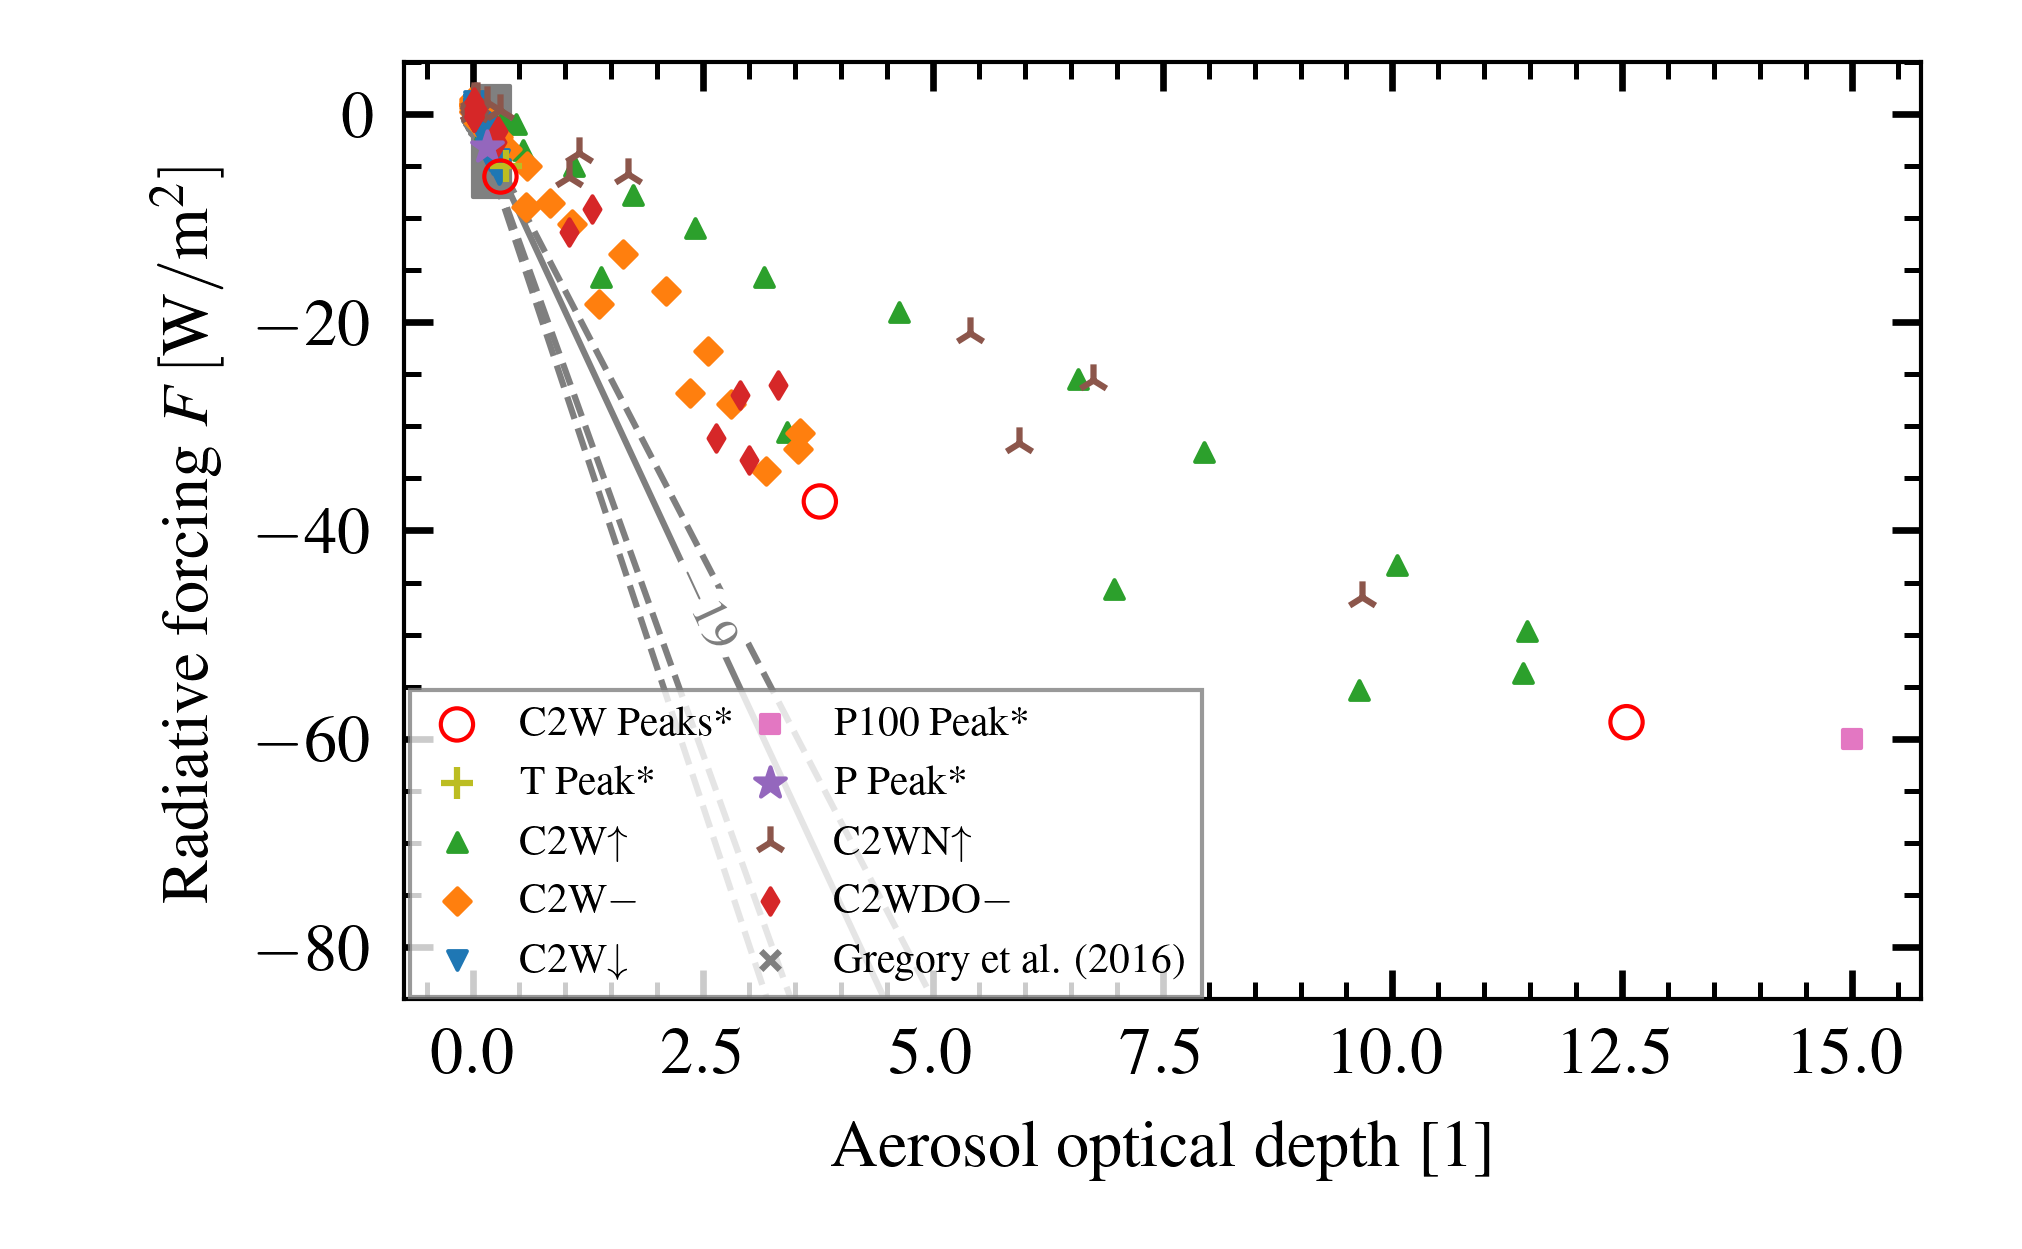
\includegraphics[width=0.95\linewidth]{figures/aod_vs_toa_avg_full.png}
  \end{center}
  \caption{\ac{aod} versus \ac{rf}, full size. Same type as
    \citet{gregory2016}}%
  \label{fig:aod_vs_toa_full}
\end{figure}

\begin{figure}[t]
  \begin{center}
    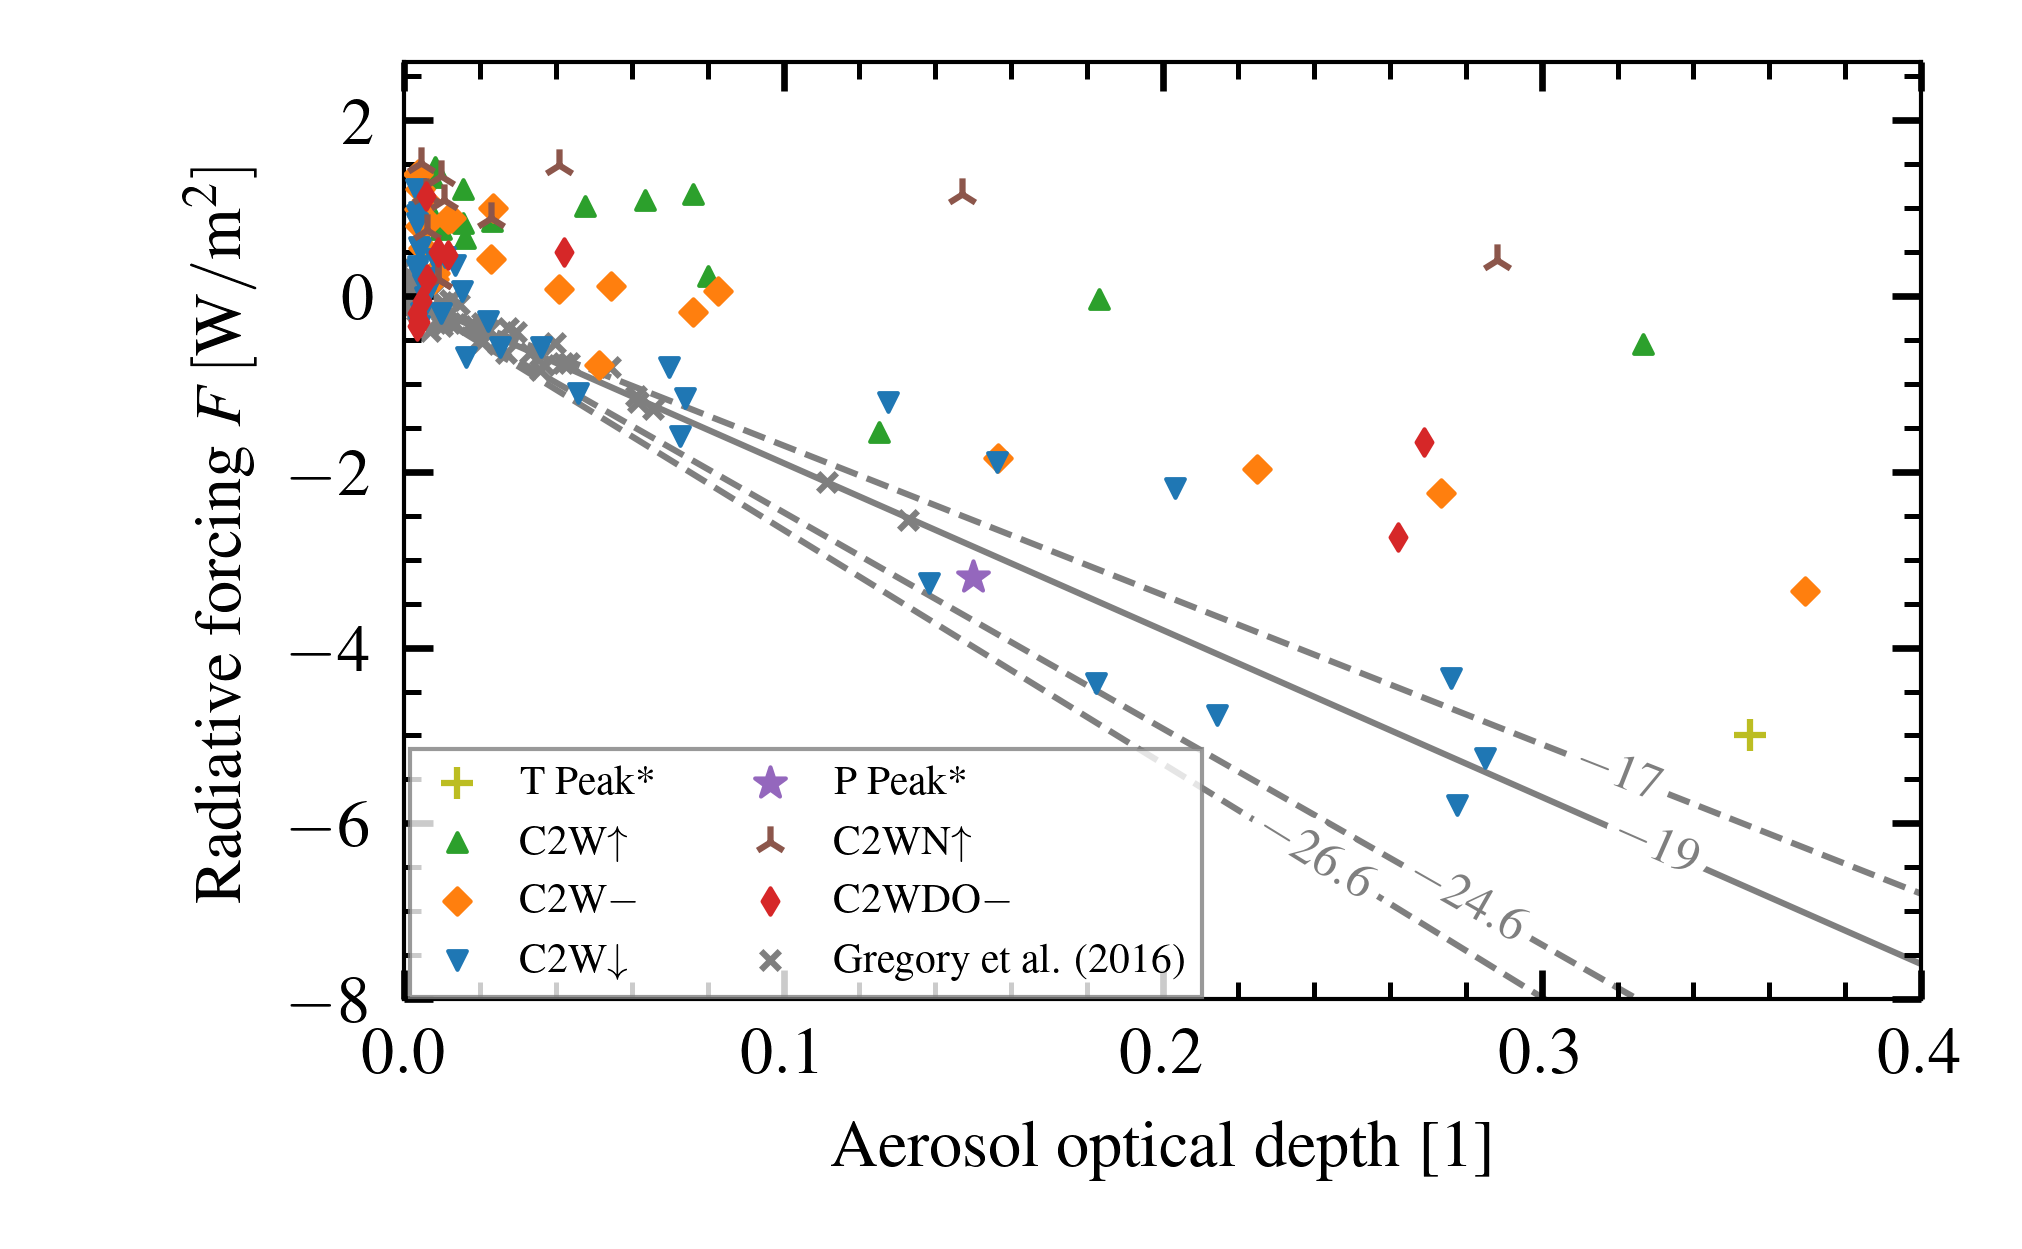
\includegraphics[width=0.95\linewidth]{figures/aod_vs_toa_avg_inset.png}
  \end{center}
  \caption{\ac{aod} versus \ac{rf}, inset. Same type as
    \citet{gregory2016}}%
  \label{fig:aod_vs_toa_inset}
\end{figure}

% \begin{figure}
%   \begin{center}
%     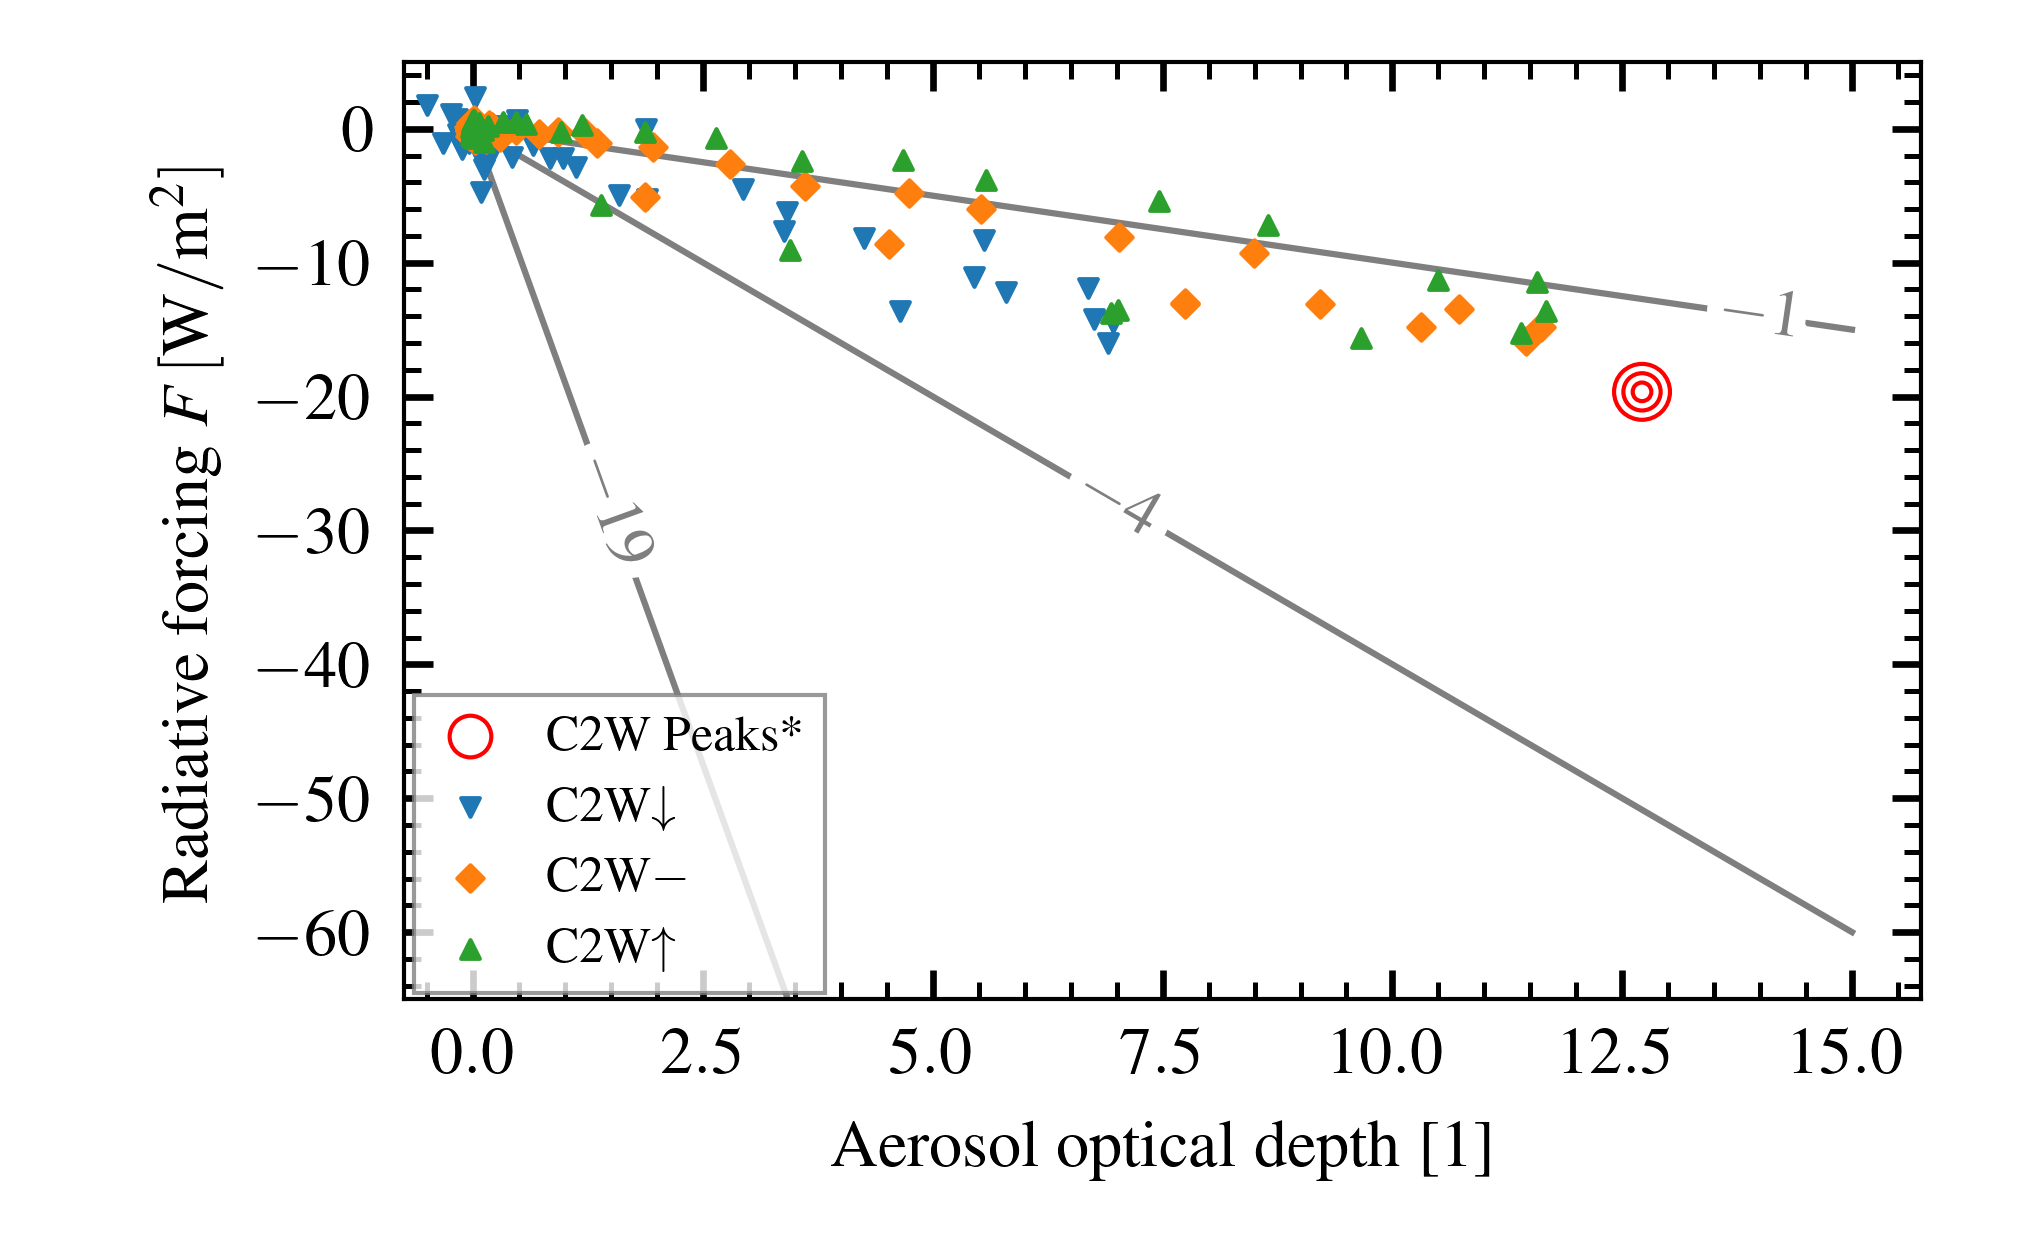
\includegraphics[width=0.95\linewidth]{figures/aod_vs_toa_avg_scaled.png}
%   \end{center}
%   \caption{
%     \ac{aod} versus \ac{rf}, scaled so the peak values of the different
%     volcano magnitudes are aligned. Same type as \citet{gregory2016}
%   }%
%   \label{fig:aod_vs_toa_scaled}
% \end{figure}

\subsection{Forcing efficiency}

To further look into the responses in \ac{aod} and \ac{rf} due to the differently sized
volcanic eruptions, we plot in
\cref{fig:aod_vs_toa_avg_loop,fig:aod_vs_toa_avg_loop_scaled,fig:aod_vs_toa_avg_loop_ratio,fig:aod_vs_toa_avg_loop_ratio_scaled}
seasonal means where the start of the time series is taken as that of the eruption day.
\Cref{fig:aod_vs_toa_avg_loop} show the four \ac{cesm2} simulations that simulates a
single volcanic eruption; three simulations cover three eruption magnitudes while the
last simulations is equivalent to the largest of the other three, but where the eruption
is located at high latitude rather than at the equator. The plot show the same picture
as \cref{fig:aod_vs_toa_full}, but the points are now seasonal means rather than yearly
means, and the colour gives the time-after-eruption. Each season has its own colour
(shown in the colour palette in the top right of the plot), except for the last year
(from \(3\) to \(4\), one colour) and the second half of the third year (from \(2.5\) to
\(3\), one colour). The later times are given fewer colour segments to better resolve
the time-after-eruption where the \ac{aod} and \ac{rf} values changes the most.
\Cref{fig:aod_vs_toa_avg_loop_scaled} show the same as \cref{fig:aod_vs_toa_avg_loop},
except the seasonal means are computed from normalized \ac{aod} and \ac{rf} time series.
\Cref{fig:aod_vs_toa_avg_loop_ratio,fig:aod_vs_toa_avg_loop_ratio_scaled} show the
\ac{rf} to \ac{aod} ratios from
\cref{fig:aod_vs_toa_avg_loop,fig:aod_vs_toa_avg_loop_scaled}, respectively. In
\cref{fig:aod_vs_toa_avg_loop_ratio}, straight lines are linear regression fits to the
seasonal means, summarised in order of the legend and from left to right in text in the
right side of the plot. Shaded regions are the standard deviation around the seasonal
means. A similar shading is plotted in \cref{fig:aod_vs_toa_avg_loop_ratio_scaled}, with
regression fits in text to the right, but where the regression lines have been omitted
to avoid further cluttering the plot.

% TODO: get out the three aerosol components to check growth and sedimentation

The ratio between \ac{aod} and \ac{rf} is not constant, and from
\cref{fig:aod_vs_toa_avg_loop} a pattern where right after the eruption \ac{rf} is
particularly strong relative to \ac{aod} show up, especially when the eruptions are very
large. \citet[][see their sections 3.1.2, 3.2.2]{marshall2019} describe how the growth
of aerosol particles affect both parameters and introduce a suggested two phases of the
aerosol evolution, a ``growth'' phase and a ``sedimentation'' phase. In general there
are larger aerosols for larger eruptions (more time to grow), such that both \ac{aod}
and \ac{rf} will be weaker (they fall out due to gravity faster and are less efficient
at scattering radiation).
% WARN: I don't know if my understanding of the following is correct
In the later phase (``sedimentation'' phase) the dependence of \ac{rf} on \ac{aod}
becomes weaker since, in addition to a faster sedimentation rate, the \ac{rf} is further
reduced due to the larger aerosols being less effective at scattering \ac{sw} radiation.
This is largely in line with the results in
\cref{fig:aod_vs_toa_avg_loop,fig:aod_vs_toa_avg_loop_scaled,fig:aod_vs_toa_avg_loop_ratio,fig:aod_vs_toa_avg_loop_ratio_scaled},
where (1) the larger eruptions have a smaller ratio (larger aerosols scatter \ac{sw}
radiation more poorly) and (2) the ratio is decreasing in magnitude as the eruption
evolve (in the early phase only, the later phase give a roughly constant ratio, see
\cref{fig:aod_vs_toa_avg_loop_ratio}). Based on the simple two phases of the aerosol
evolution \citep{marshall2019}, an increasing \ac{rf} to \ac{aod} ratio (decreasing when
considering absolute values) seems reasonable.

\citet[][their figure 1c,d]{marshall2020} present results showing a time dependence in
the conversion between \ac{aod} and \ac{rf}, but where \ac{rf} is larger (more
efficient) later in the eruption evolution when compared to \ac{aod}, not smaller. This
happen since the aerosols are initially spatially confined to the hemisphere where the
eruption was situated, leading to a larger global mean albedo per \ac{aod} and in turn
large \ac{rf} per \ac{aod} \citep{marshall2020}. From their results and the results
shown here in
\cref{fig:aod_vs_toa_avg_loop,fig:aod_vs_toa_avg_loop_scaled,fig:aod_vs_toa_avg_loop_ratio,fig:aod_vs_toa_avg_loop_ratio_scaled},
there seems to be several and competing effects that decide on the values of \ac{aod}
and \ac{rf}.

\begin{figure}[t]
  \begin{center}
    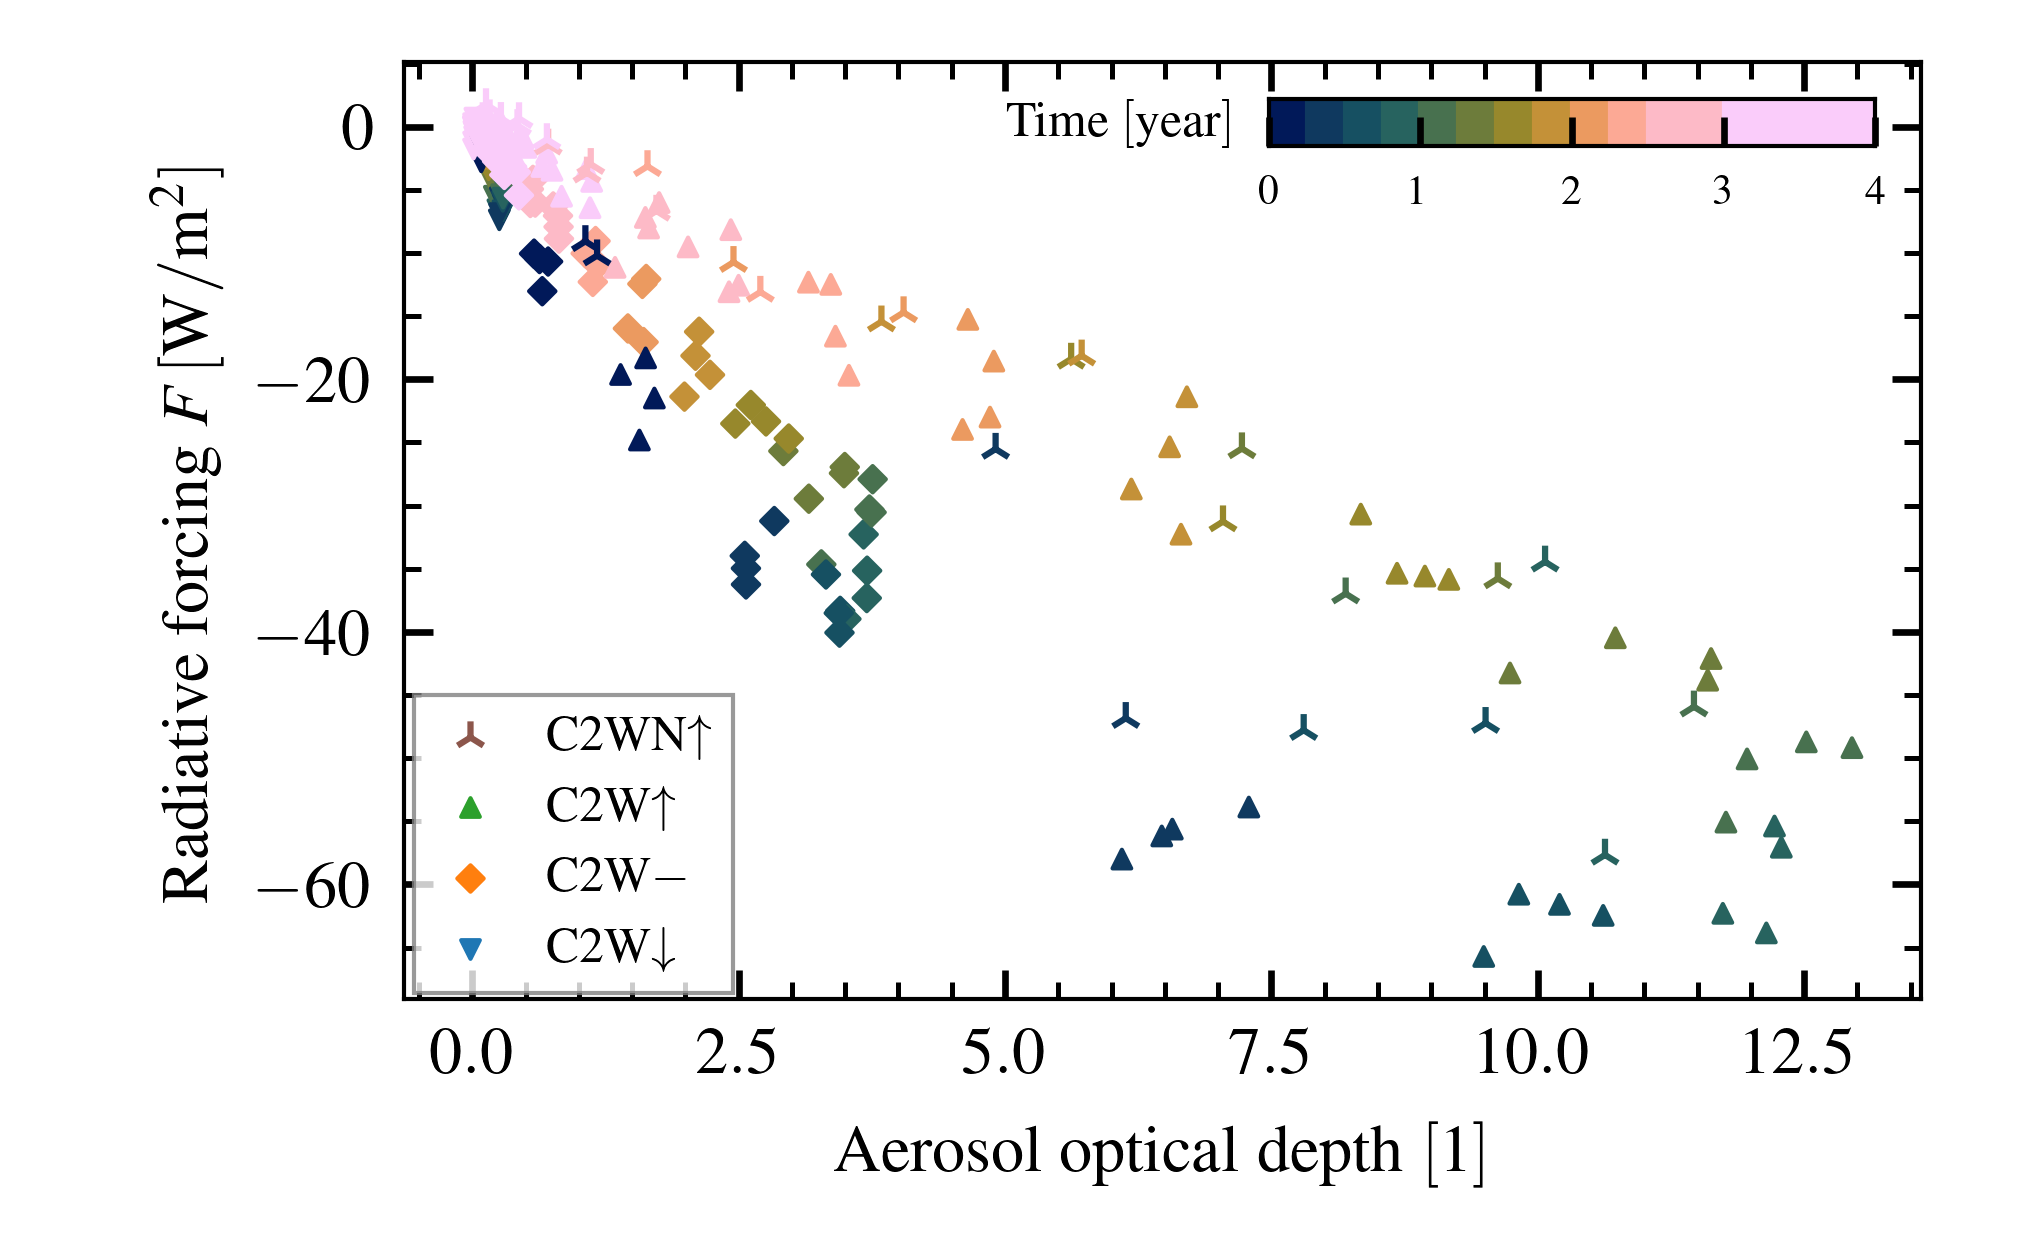
\includegraphics[width=0.95\linewidth]{figures/aod_vs_toa_avg_loop.png}
  \end{center}
  \caption{
    \ac{aod} versus \ac{rf}, with points coloured according to the year and
    season it was averaged from. (Same type of plot as \citet{gregory2016})
  }%
  \label{fig:aod_vs_toa_avg_loop}
\end{figure}

\begin{figure}[t]
  \begin{center}
    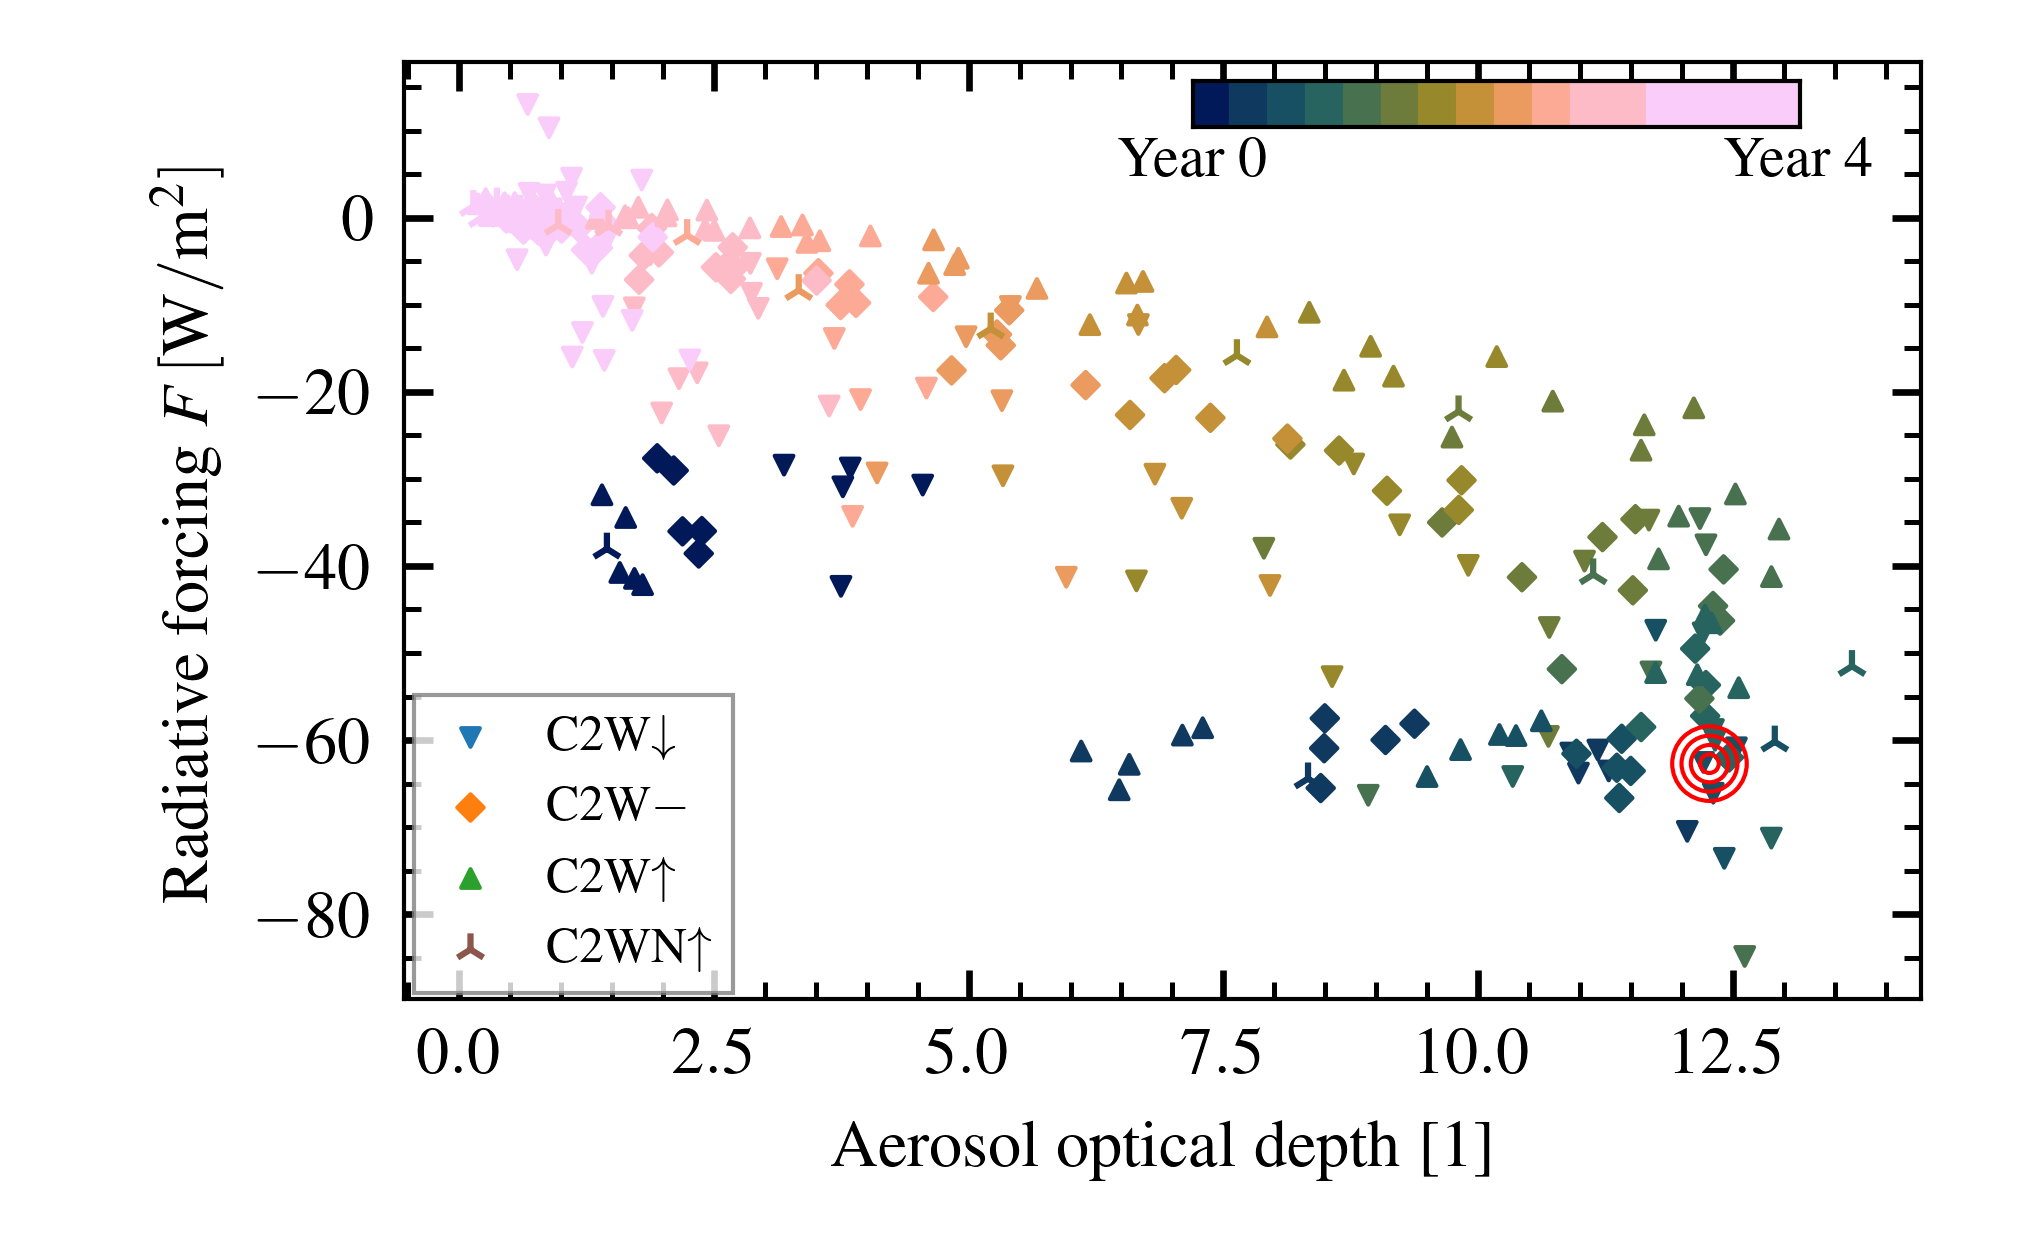
\includegraphics[width=0.95\linewidth]{figures/aod_vs_toa_avg_loop_scaled.png}
  \end{center}
  \caption{
    \ac{aod} versus \ac{rf}, with points coloured according to the year and
    season it was averaged from, and scaled so the peak values are aligned. (Same type
    of plot as \citet{gregory2016})
  }%
  \label{fig:aod_vs_toa_avg_loop_scaled}
\end{figure}

In \cref{fig:aod_vs_toa_avg_loop_ratio} we plot the ratio of the annual means of \ac{rf}
and \ac{aod}. The years where the signal-to-noise ratio is the lowest are years 1 and 2,
as well as year 0 (the noise is mostly due to the \ac{rf} time series, shown in
\cref{fig:toa_arrays_normalized}). For this reason, the ratio of \ac{rf} to \ac{aod} is
calculated for the second season of the first year until the end of the third year. From
this we find that even though the ratio changes between the eruption magnitudes, we find
that the gradient at which the ratio is changing is similar across large eruption
magnitudes. A slope of approximately \( 5.8 \) is a good fit for both the intermediate
(orange thick diamonds) and the strong eruption (green upward triangles), and even
though the spread in the small eruption (blue downward triangles) is large in the \( y
\)-direction, they tend to follow a similarly inclined, albeit steeper, slope. In the
later phase, from the second season of the second year, the ratios stay close to
constant for the reminder of the decaying phase.

The change in ratio, where the smallest is found in the strong eruption and the largest
ratio is from the small eruption, is consistent with the change in peak values seen in
\cref{fig:aod_vs_toa_full}, where the red circles indicate that the peak values are
saturating. The \ac{rf} peak magnitudes increases more slowly than the \ac{aod} peak
magnitudes which increases close to linearly with injected \ce{SO2} (see also
\cref{fig:so2_vs_aod}). This may be the result of larger aerosols having time to develop
as the amount of injected \ce{SO2} increases \citep{niemeier2015,marshall2019}. This in
turn make the forcing from smaller eruptions relatively more efficient than from large
eruptions since larger aerosols scatter radiation less efficiently, causing a less
negative ratio between \ac{rf} and \ac{aod}.

\begin{figure}[t]
  \begin{center}
    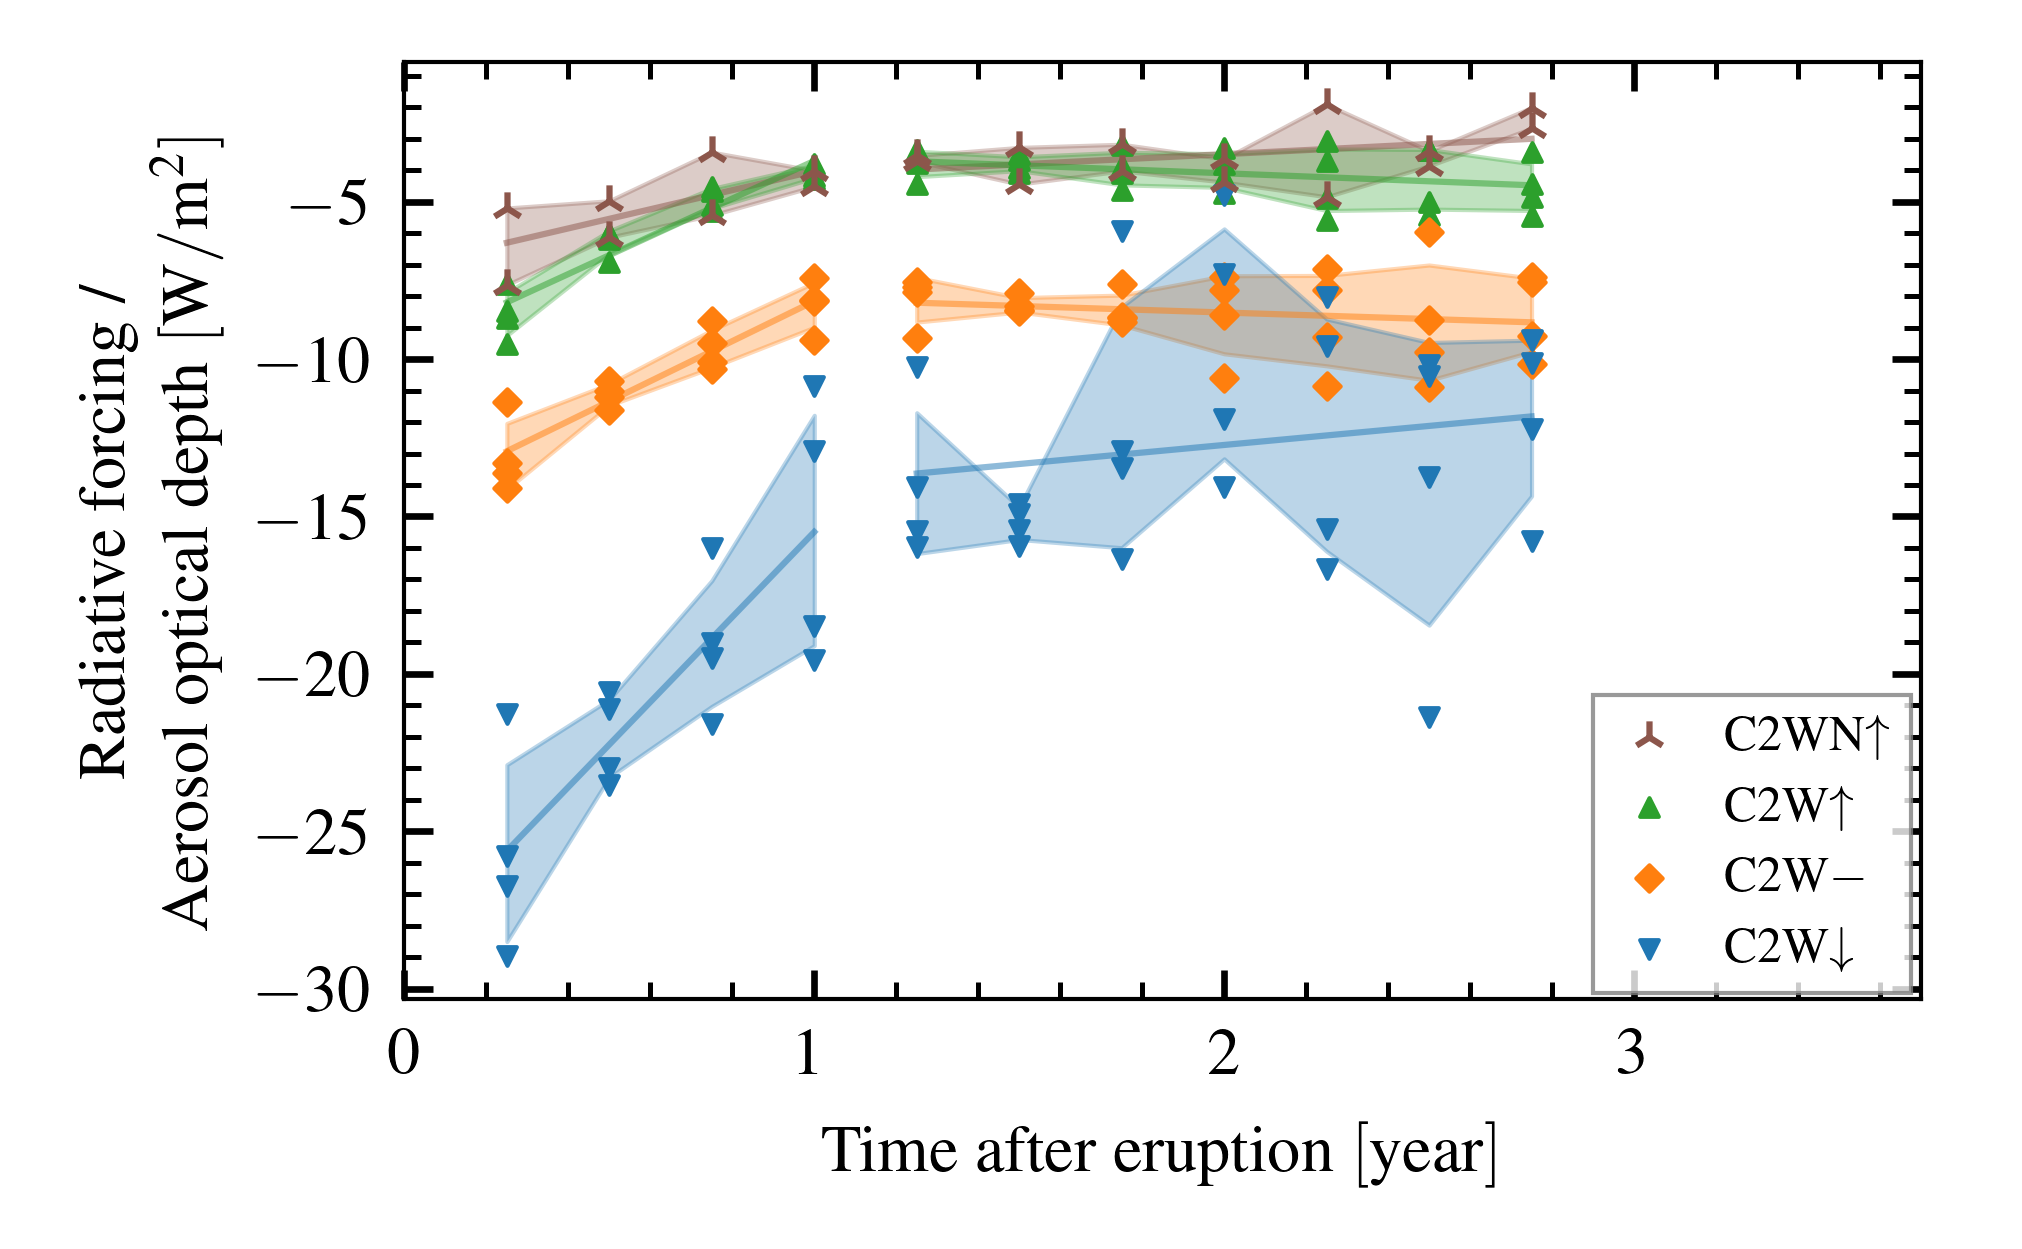
\includegraphics[width=0.95\linewidth]{figures/aod_vs_toa_avg_loop_ratio.png}
  \end{center}
  \caption{
    Ratio of \ac{rf} to \ac{aod} as shown in
    \cref{fig:aod_vs_toa_avg_loop}, with the time-after-eruption on the horizontal axis.
    Slopes are linear regression fits using \textbf{scipy}
  }%
  \label{fig:aod_vs_toa_avg_loop_ratio}
\end{figure}

\begin{figure}[t]
  \begin{center}
    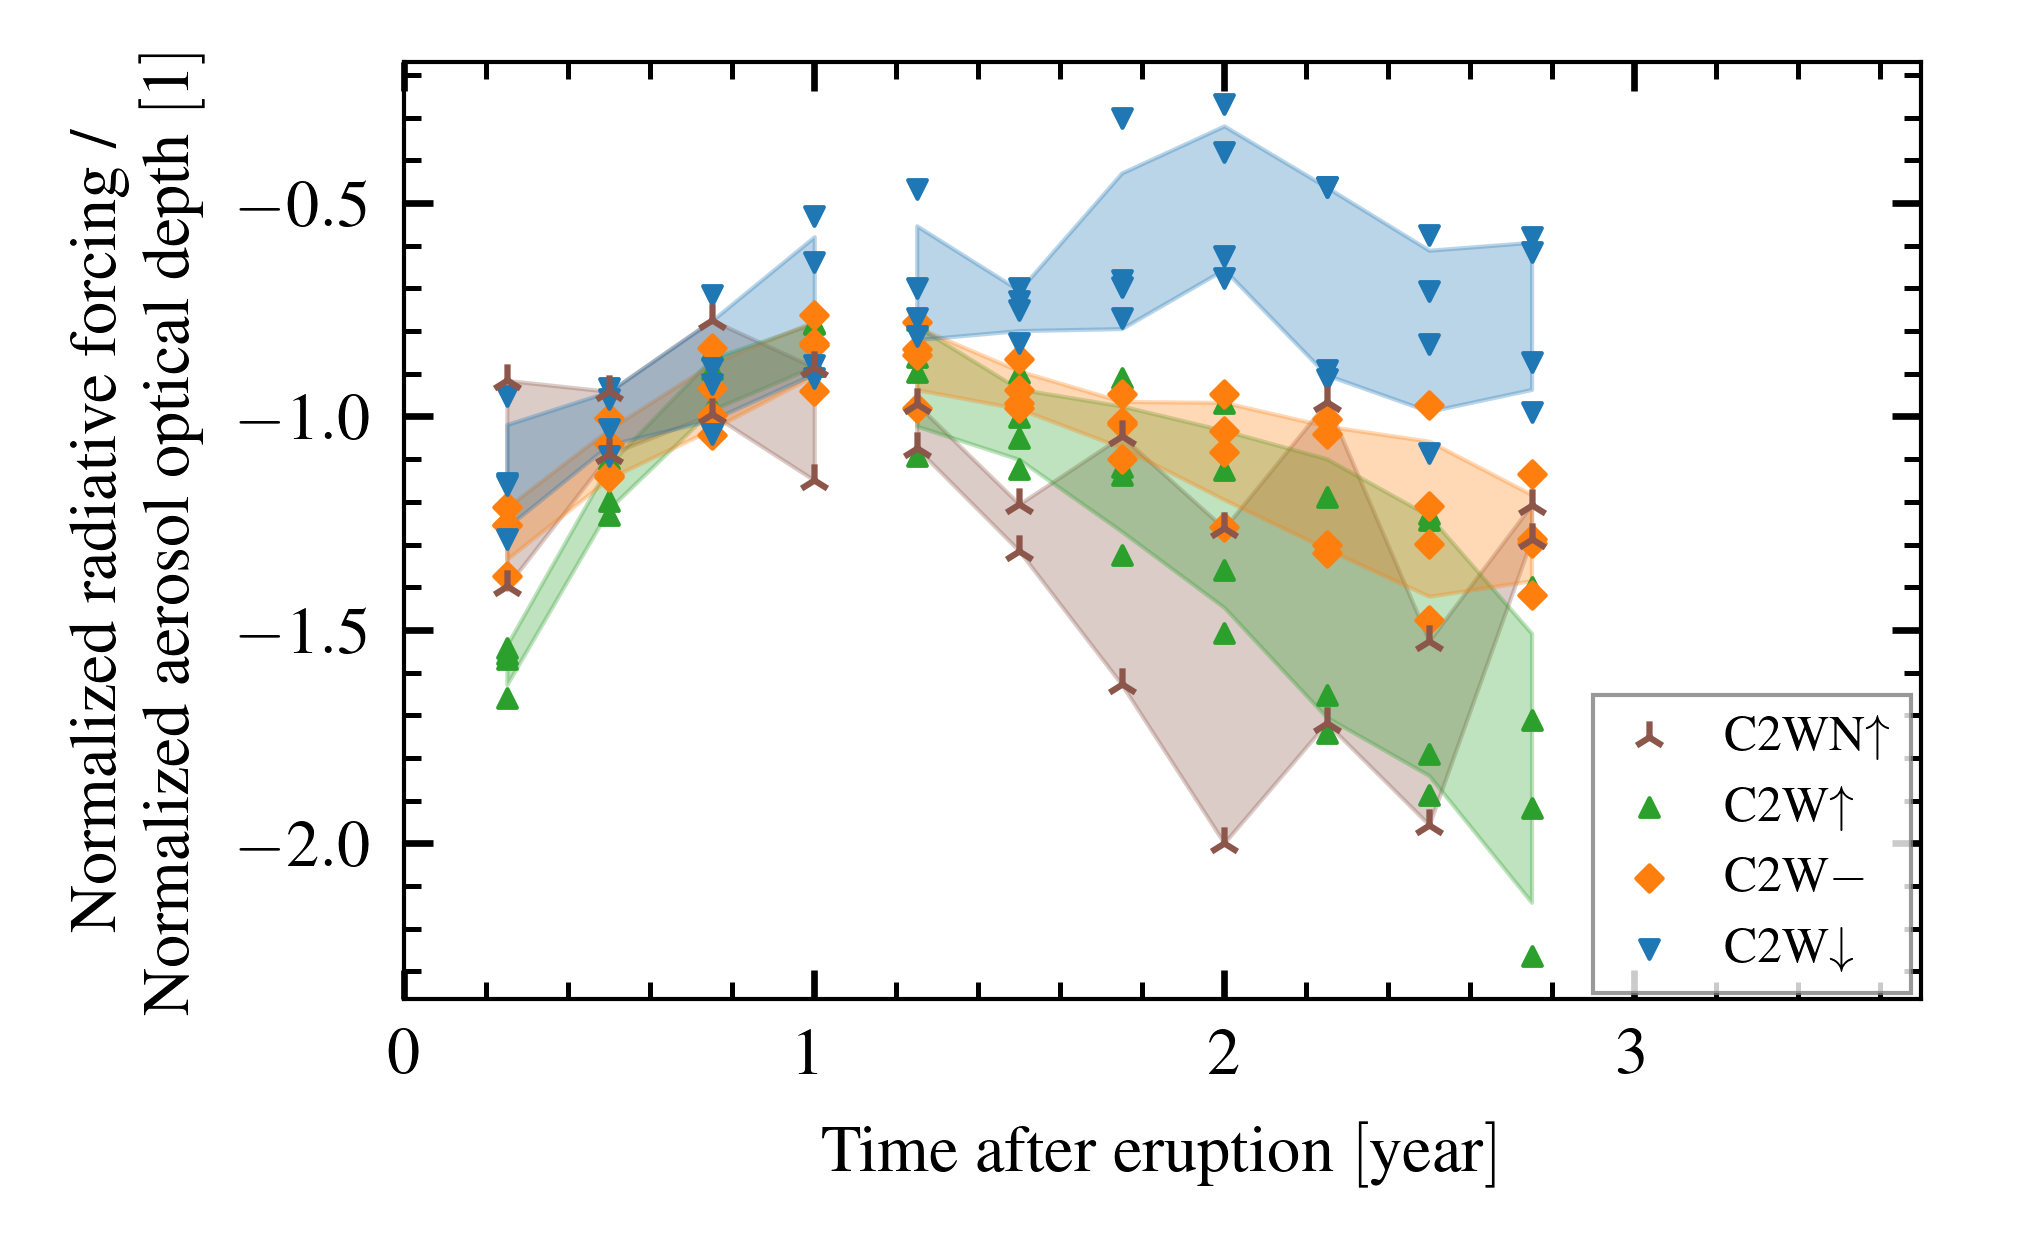
\includegraphics[width=0.95\linewidth]{figures/aod_vs_toa_avg_loop_ratio_scaled.png}
  \end{center}
  \caption{
    A scaled version of \cref{fig:aod_vs_toa_avg_loop_ratio}, where the scaling is the
    exact same as in \cref{fig:aod_vs_toa_avg_loop_scaled} compared to
    \cref{fig:aod_vs_toa_avg_loop}
  }%
  \label{fig:aod_vs_toa_avg_loop_ratio_scaled}
\end{figure}

One feature seen in \cref{fig:aod_vs_toa_avg_loop,fig:aod_vs_toa_avg_loop_ratio} is that
the early phase seems to have a \ac{rf} to \ac{aod} ratio that is changing (from about
\(0\) to \(1.2\) years after the eruption), while the later phase has an almost constant
ratio (from \(1.2\) to \(3\)--\(4\) years after the eruption). When plotting the \ac{rf}
time series, we find that their shapes are very consistent over different eruption
strengths (\cref{fig:toa_arrays_normalized}), but the \ac{aod} time series show a slight
change in shape from smaller to larger eruptions (\cref{fig:aod_arrays_normalized}).
Specifically, the \ac{aod} time series from the smallest eruptions have a fast rise and
a flat peak before it decays back to its equilibrium state, while from the two larger
eruptions we find a slower rise time, but a sharper peak, making the decay to
equilibrium happening at a similar time after the eruption and at a similar rate.
% TODO: Why? Marshall et al. (2019) and references therein may be the best source for a
% suggested explanation.

An interesting aspect concerning the similar decaying phase seen in both the \ac{aod}
time series and the \ac{rf} time series is the influence of these decaying phases on the
temperature time series, perhaps inducing a trend. That is, do the temperature time
series have different shape in the rising phase, but similar shape in the decaying
phase, as discussed in relation to \cref{fig:temp_norm_max,fig:temp_norm_int}. Allowing
the simulations to run for at least twenty years to allow the tail to be well resolved
is therefore another avenue that could be explored further.
% WARN: The paragraph above is left hanging... Although it is connected to the next
% section.

\begin{figure}[t]
  \begin{center}
    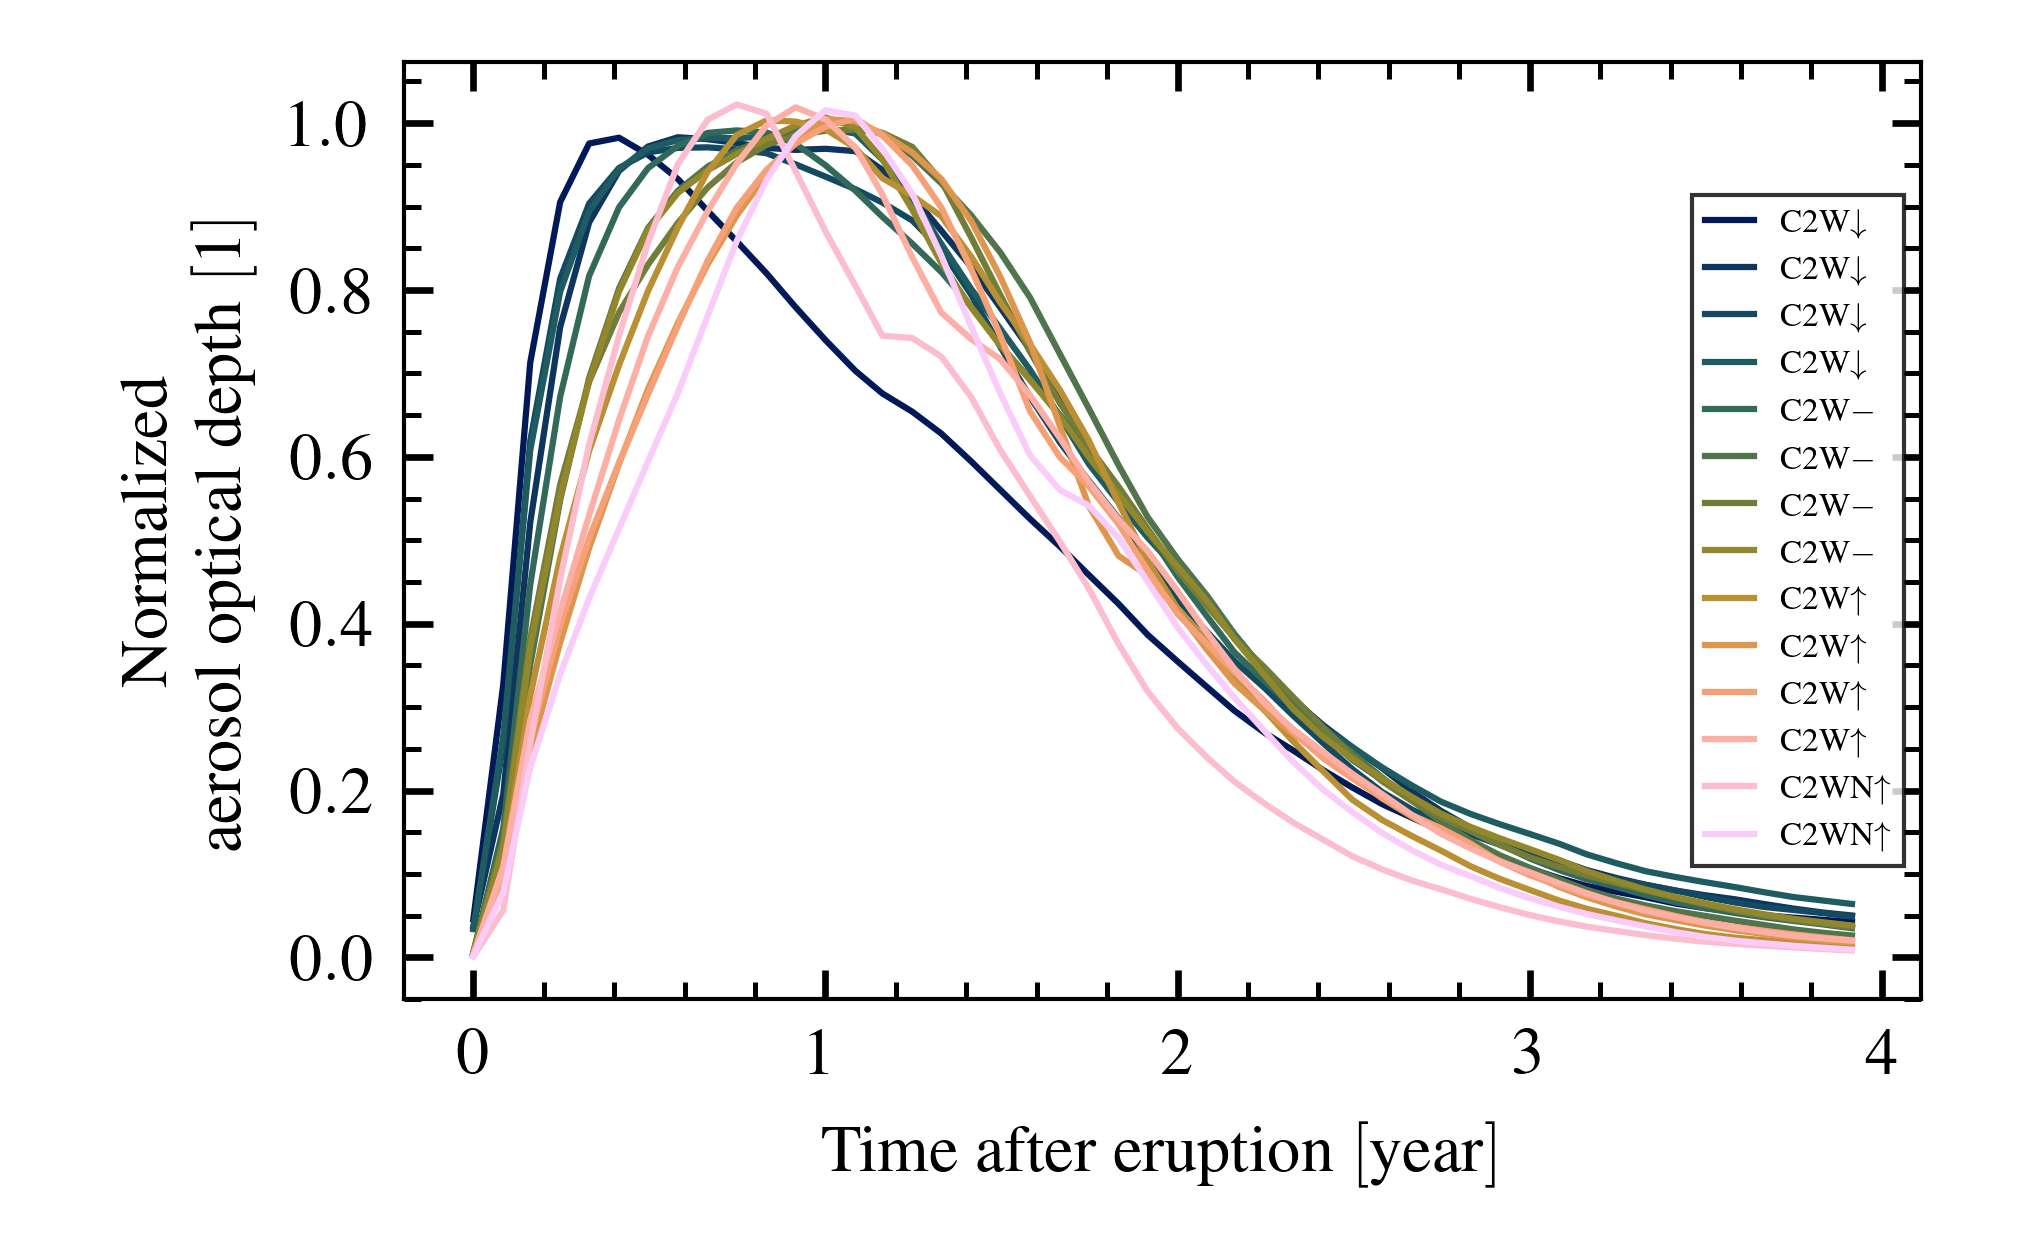
\includegraphics[width=0.95\linewidth]{figures/aod_arrays_normalized.png}
  \end{center}
  \caption{
    The (scaled versions of the) arrays used in
    \cref{fig:aod_vs_toa_avg_loop_scaled,fig:aod_vs_toa_avg_loop_ratio_scaled}
    (\cref{fig:aod_vs_toa_avg_loop,fig:aod_vs_toa_avg_loop_ratio})
  }%
  \label{fig:aod_arrays_normalized}
\end{figure}

\begin{figure}[t]
  \begin{center}
    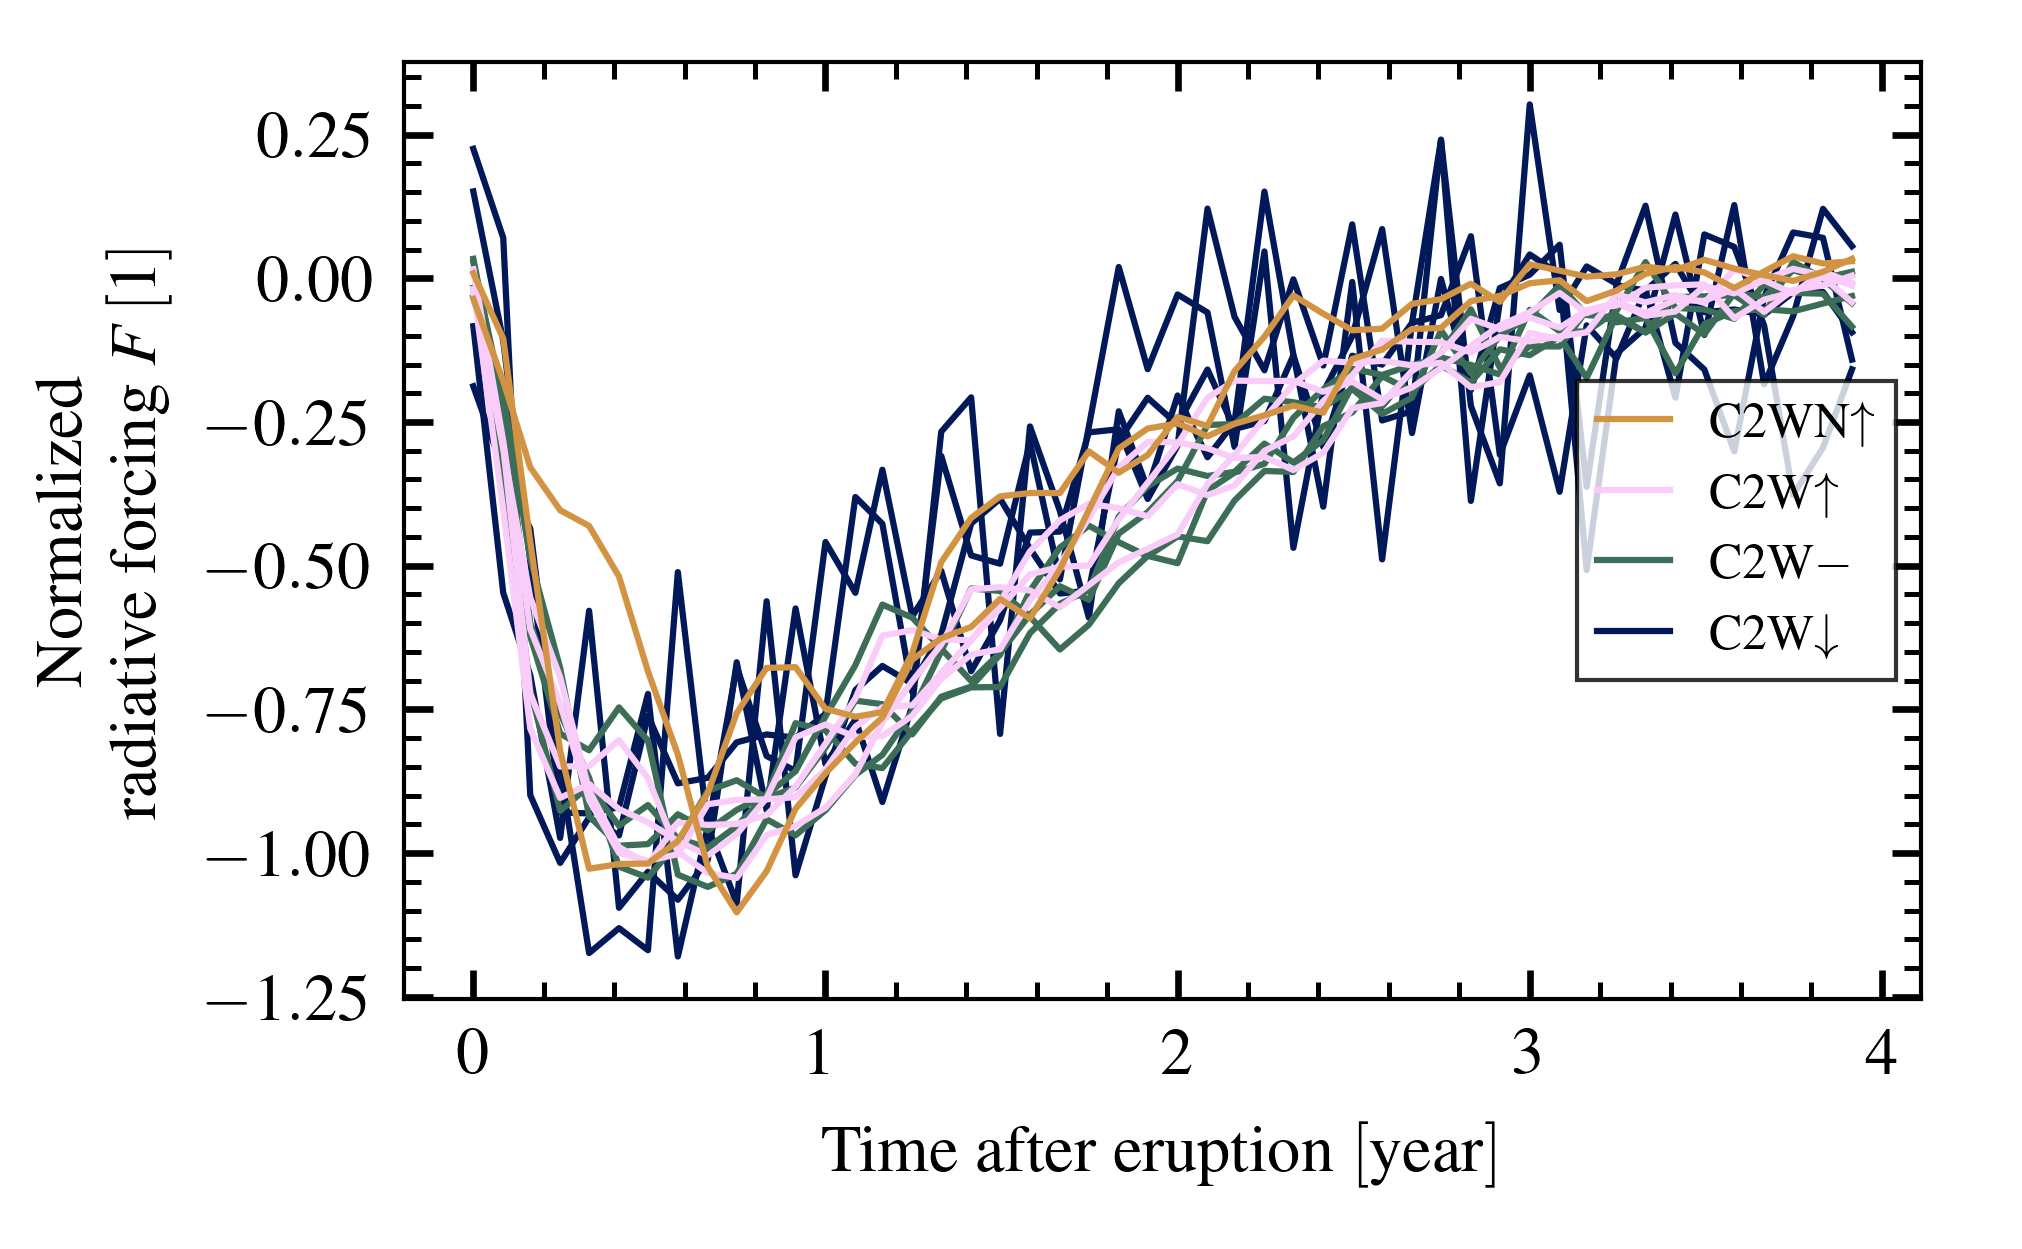
\includegraphics[width=0.95\linewidth]{figures/toa_arrays_normalized.png}
  \end{center}
  \caption{
    The (scaled versions of the) arrays used in
    \cref{fig:aod_vs_toa_avg_loop_scaled,fig:aod_vs_toa_avg_loop_ratio_scaled}
    (\cref{fig:aod_vs_toa_avg_loop,fig:aod_vs_toa_avg_loop_ratio})
  }%
  \label{fig:toa_arrays_normalized}
\end{figure}

\subsection{Forcing magnitudes}

Whether the different shapes of the temperature time series can be obtained (synonyms?)
from the shape of either of the forcing time series or not (\ac{rf} or \ac{aod}) is a
natural next step to take. There are three different forcing magnitudes that have been
used, as outlined in \cref{tab:simulation-overview}. The figures below show two
alternative ways of normalizing the temperature response to these volcanic forcing
events. First, the three temperature responses are normalized by setting the smoothed
peak\footnote{the peak of a third-order Savitzky-Golay filter with a one year long
  window length} value equal to one, shown in \cref{fig:temp_norm_max}. The second method
of normalizing, shown in \cref{fig:temp_norm_int}, is to divide by the integral of the
time series, such that the scaled time series integrate to one.

When normalizing by setting their amplitude equal to (minus) one, the initial rise
across all three time series is comparable. The difference among the three is how
quickly the temperature reverts back to equilibrium in the small eruption case (solid
black and blue shading in \cref{fig:temp_norm_max}). On the other hand, when normalizing
by enforcing all time series to integrate to the same value, the tails of the
temperature time series by construction become similar across the three eruption
magnitudes. From both of these two normalizations, the amount of time spent at the peak
temperature appears different. The temperature from the smaller eruption simulation
starts to revert sooner after it reaches the peak temperature. The shape of the initial
rise and the tail is more similar across the three, while the peak is sharper in the
small eruption case compared to the two larger.

% NOTE: Any similar results that is consistent with a faster temperature recovery for
% weaker volcanic forcing? Not, sure, but one curiosity is that in the AOD signals, the
% smaller eruption spent more time at the peak, contrary to what seems to be the case
% for the temperature. The RF time series have similar shape for all forcing magnitudes.
% See figs. 9 (aod_arrays_normalized) and 10 (toa_arrays_normalized).

\begin{figure}[t]
  \begin{center}
    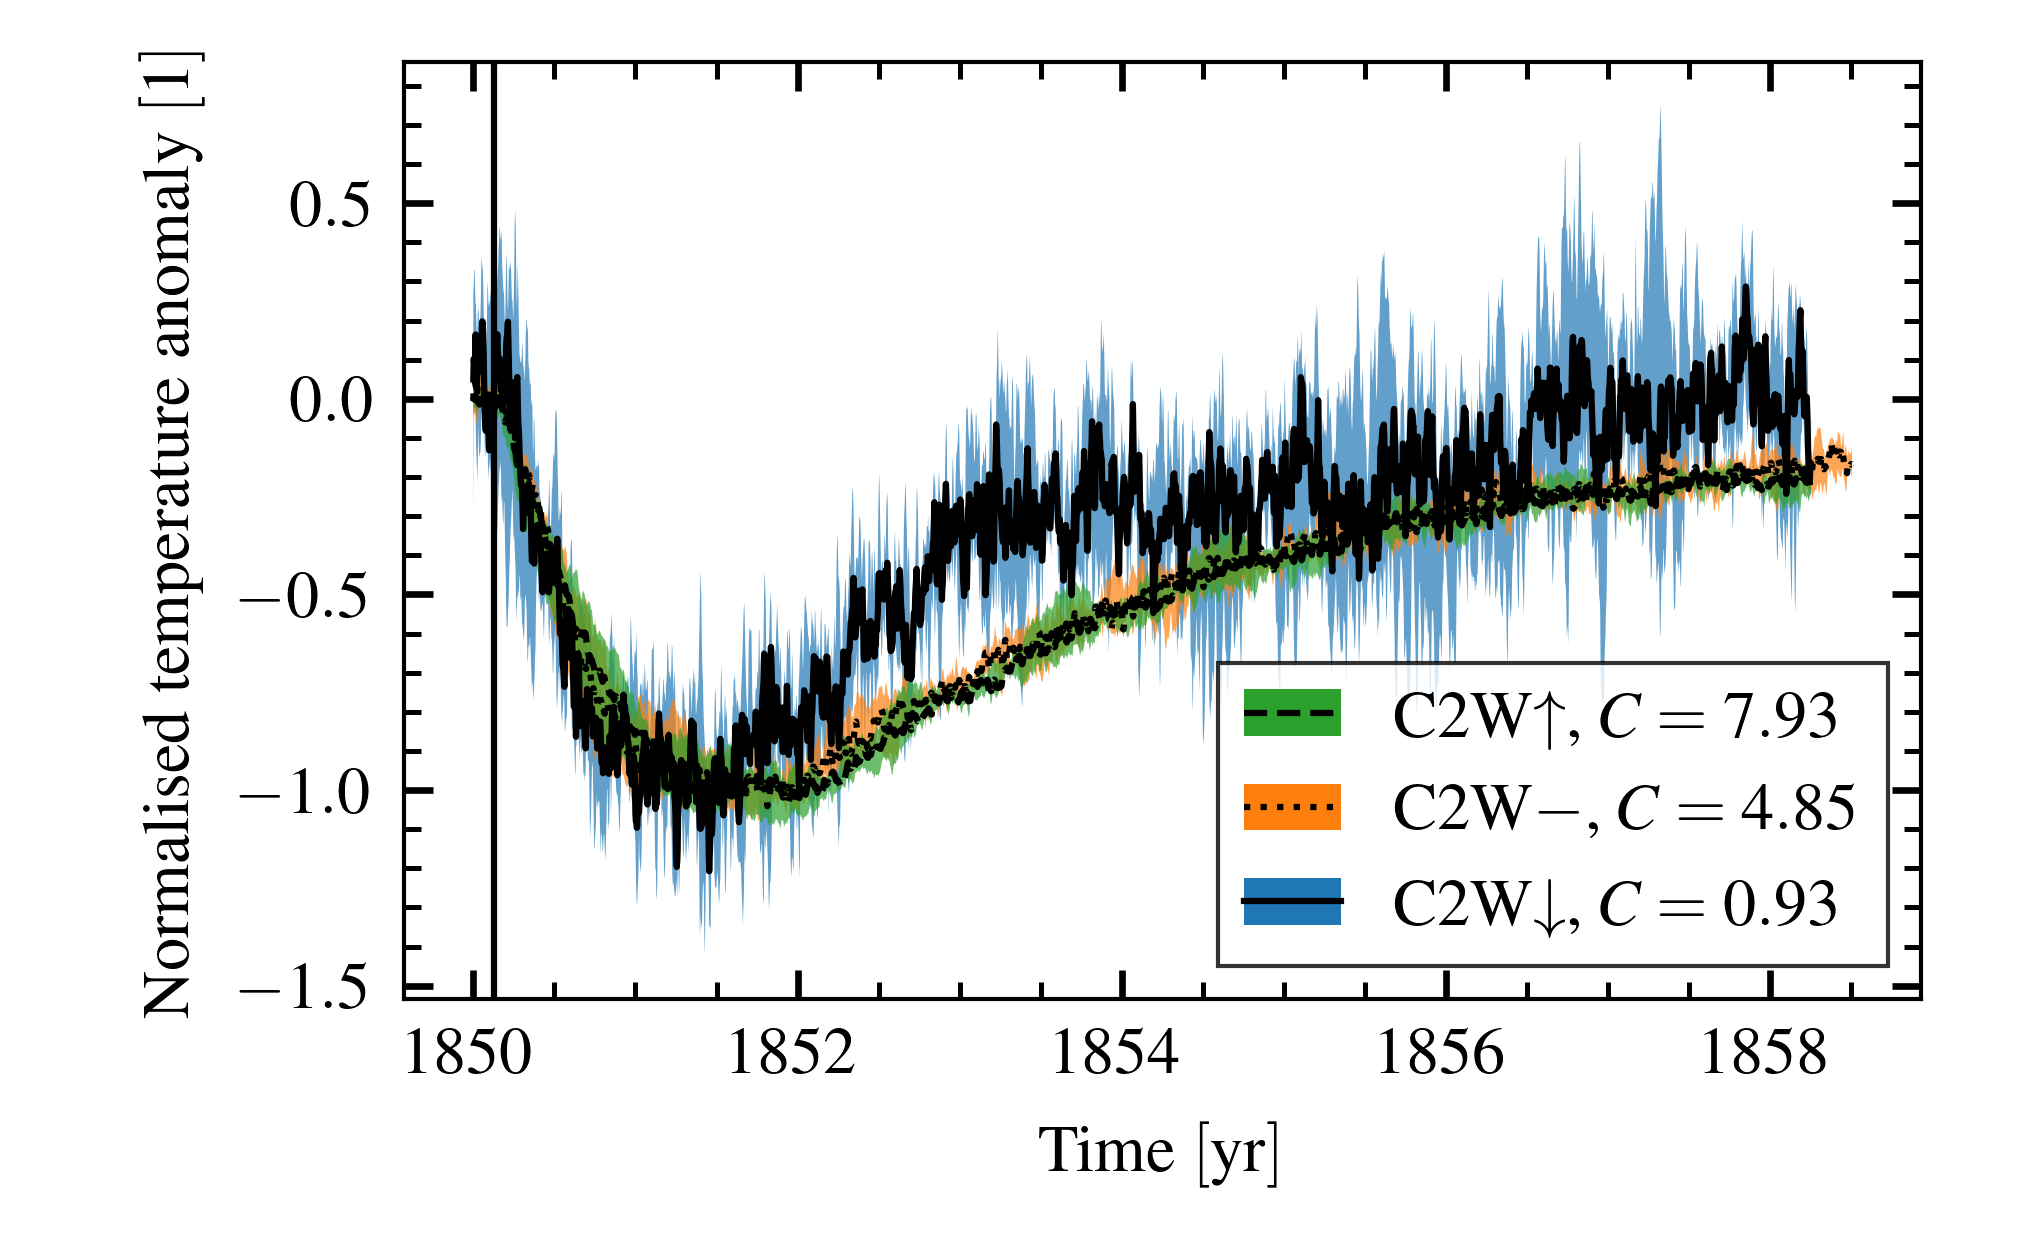
\includegraphics[width=0.95\linewidth]{figures/compare-waveform-max.png}
  \end{center}
  \caption{Normalized temperature response to three different-size volcanic eruptions,
    by setting a maximum peak value}%
  \label{fig:temp_norm_max}
\end{figure}

\begin{figure}[t]
  \begin{center}
    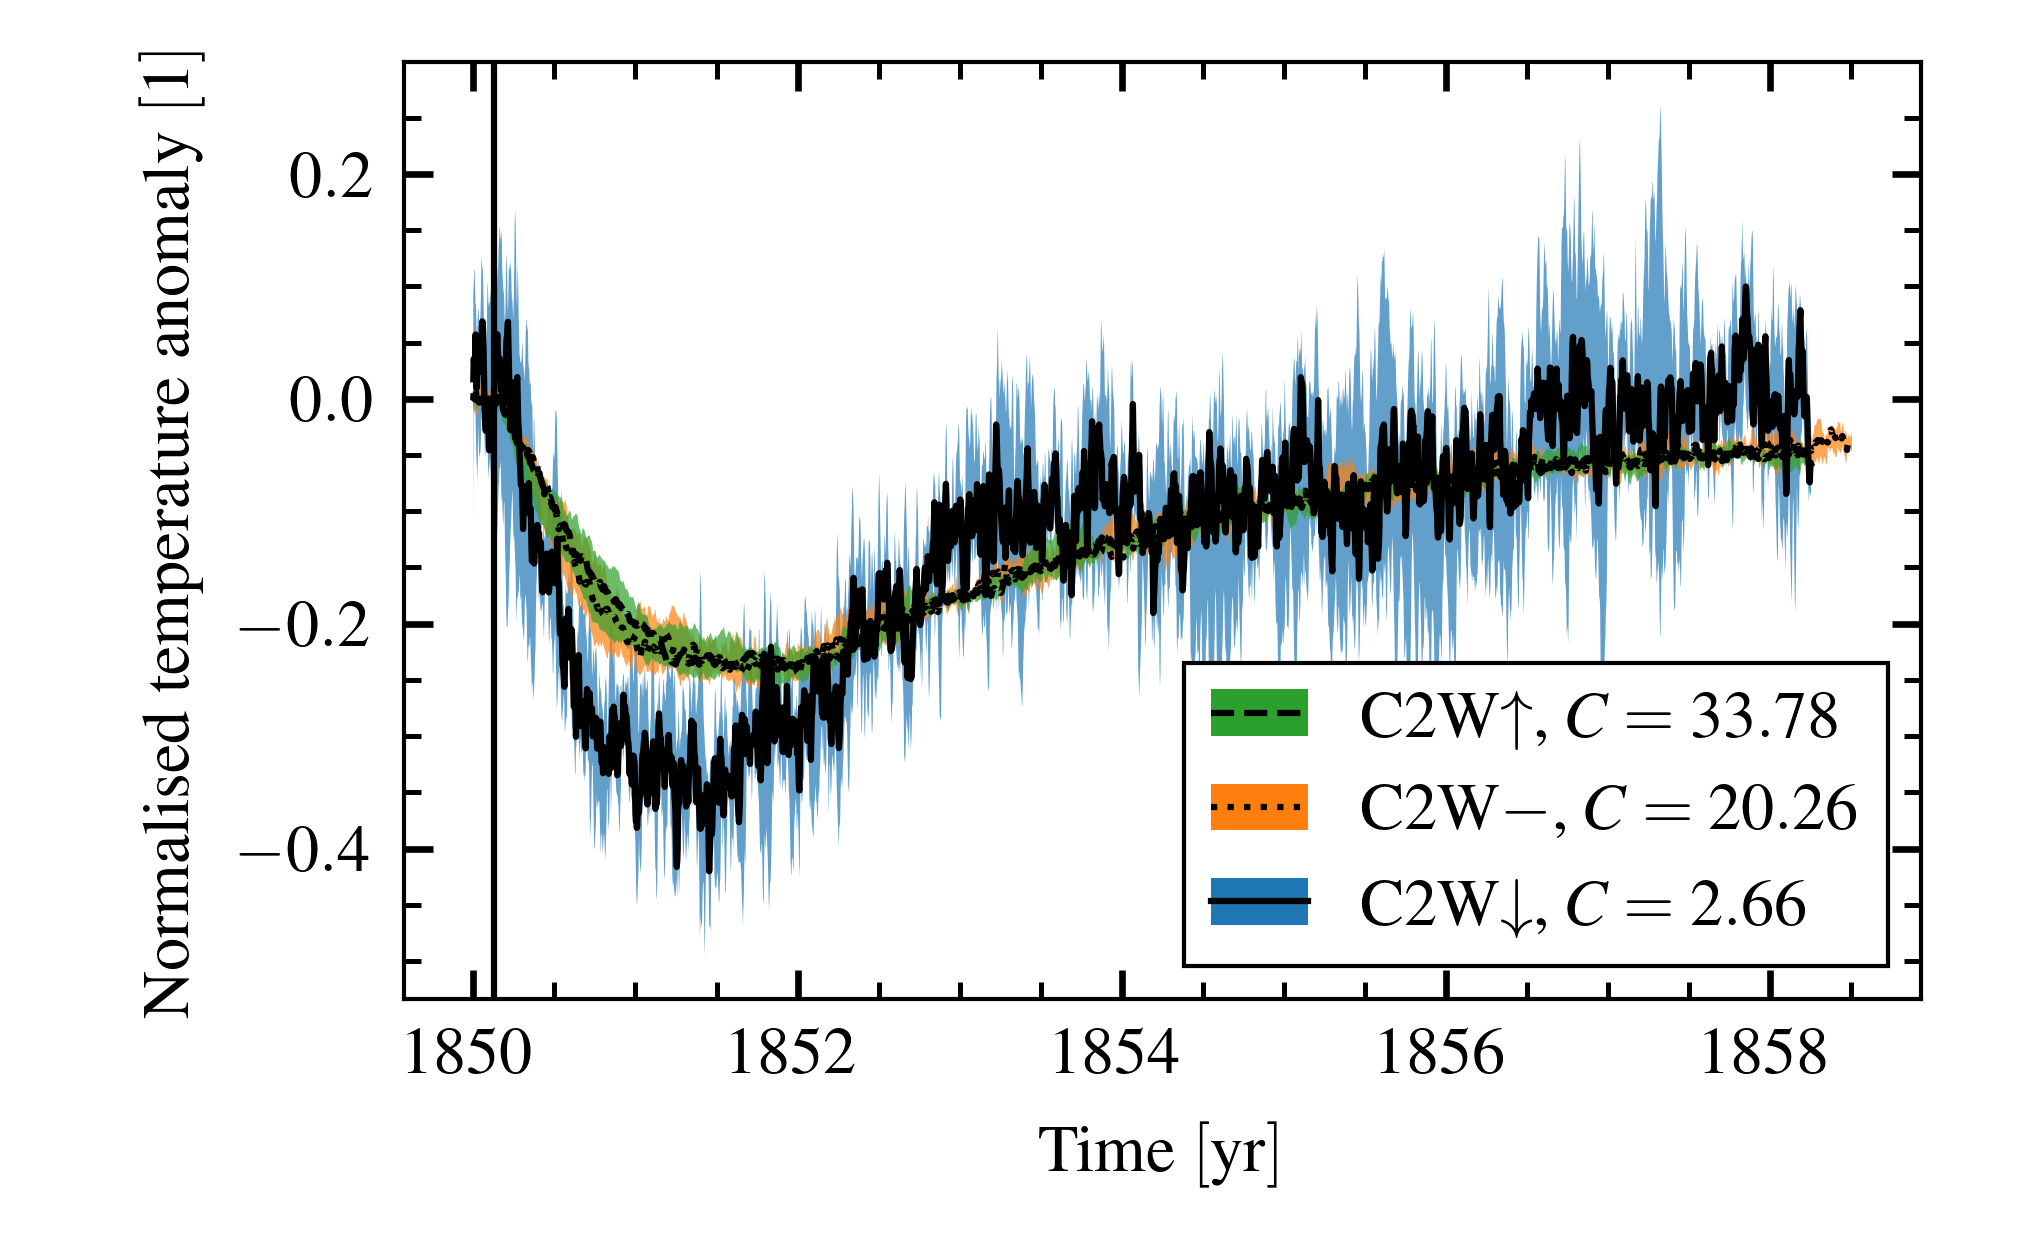
\includegraphics[width=0.95\linewidth]{figures/compare-waveform-integrate.png}
  \end{center}
  \caption{Normalized temperature response to three different-size volcanic eruptions,
    using integration, i.e., they all integrate to one}%
  \label{fig:temp_norm_int}
\end{figure}

\subsection{Comparing parameters}

Finally we compare all relevant parameters to each other. The initial input parameter to
the \ac{cesm2} is injected \ce{SO2}. Compared to \ac{aod} peak values we get an almost
linear relationship against \iso{}, shown in \cref{fig:so2_vs_aod}.\footnote{\emph{Since
    \iso{} is ``total amount of \iso{}'', maybe consider comparing to integrated values of
    \ac{aod}, \ac{rf} and temperature as well, not just the peak values.}} The latitude also
plays a role for how large the \ac{aod} perturbation becomes, as we can see from the
\ac{c2wsn} data point. The weak dependence on eruption latitude is also reported in
\citet{marshall2019}.

\begin{figure}[t]
  \begin{center}
    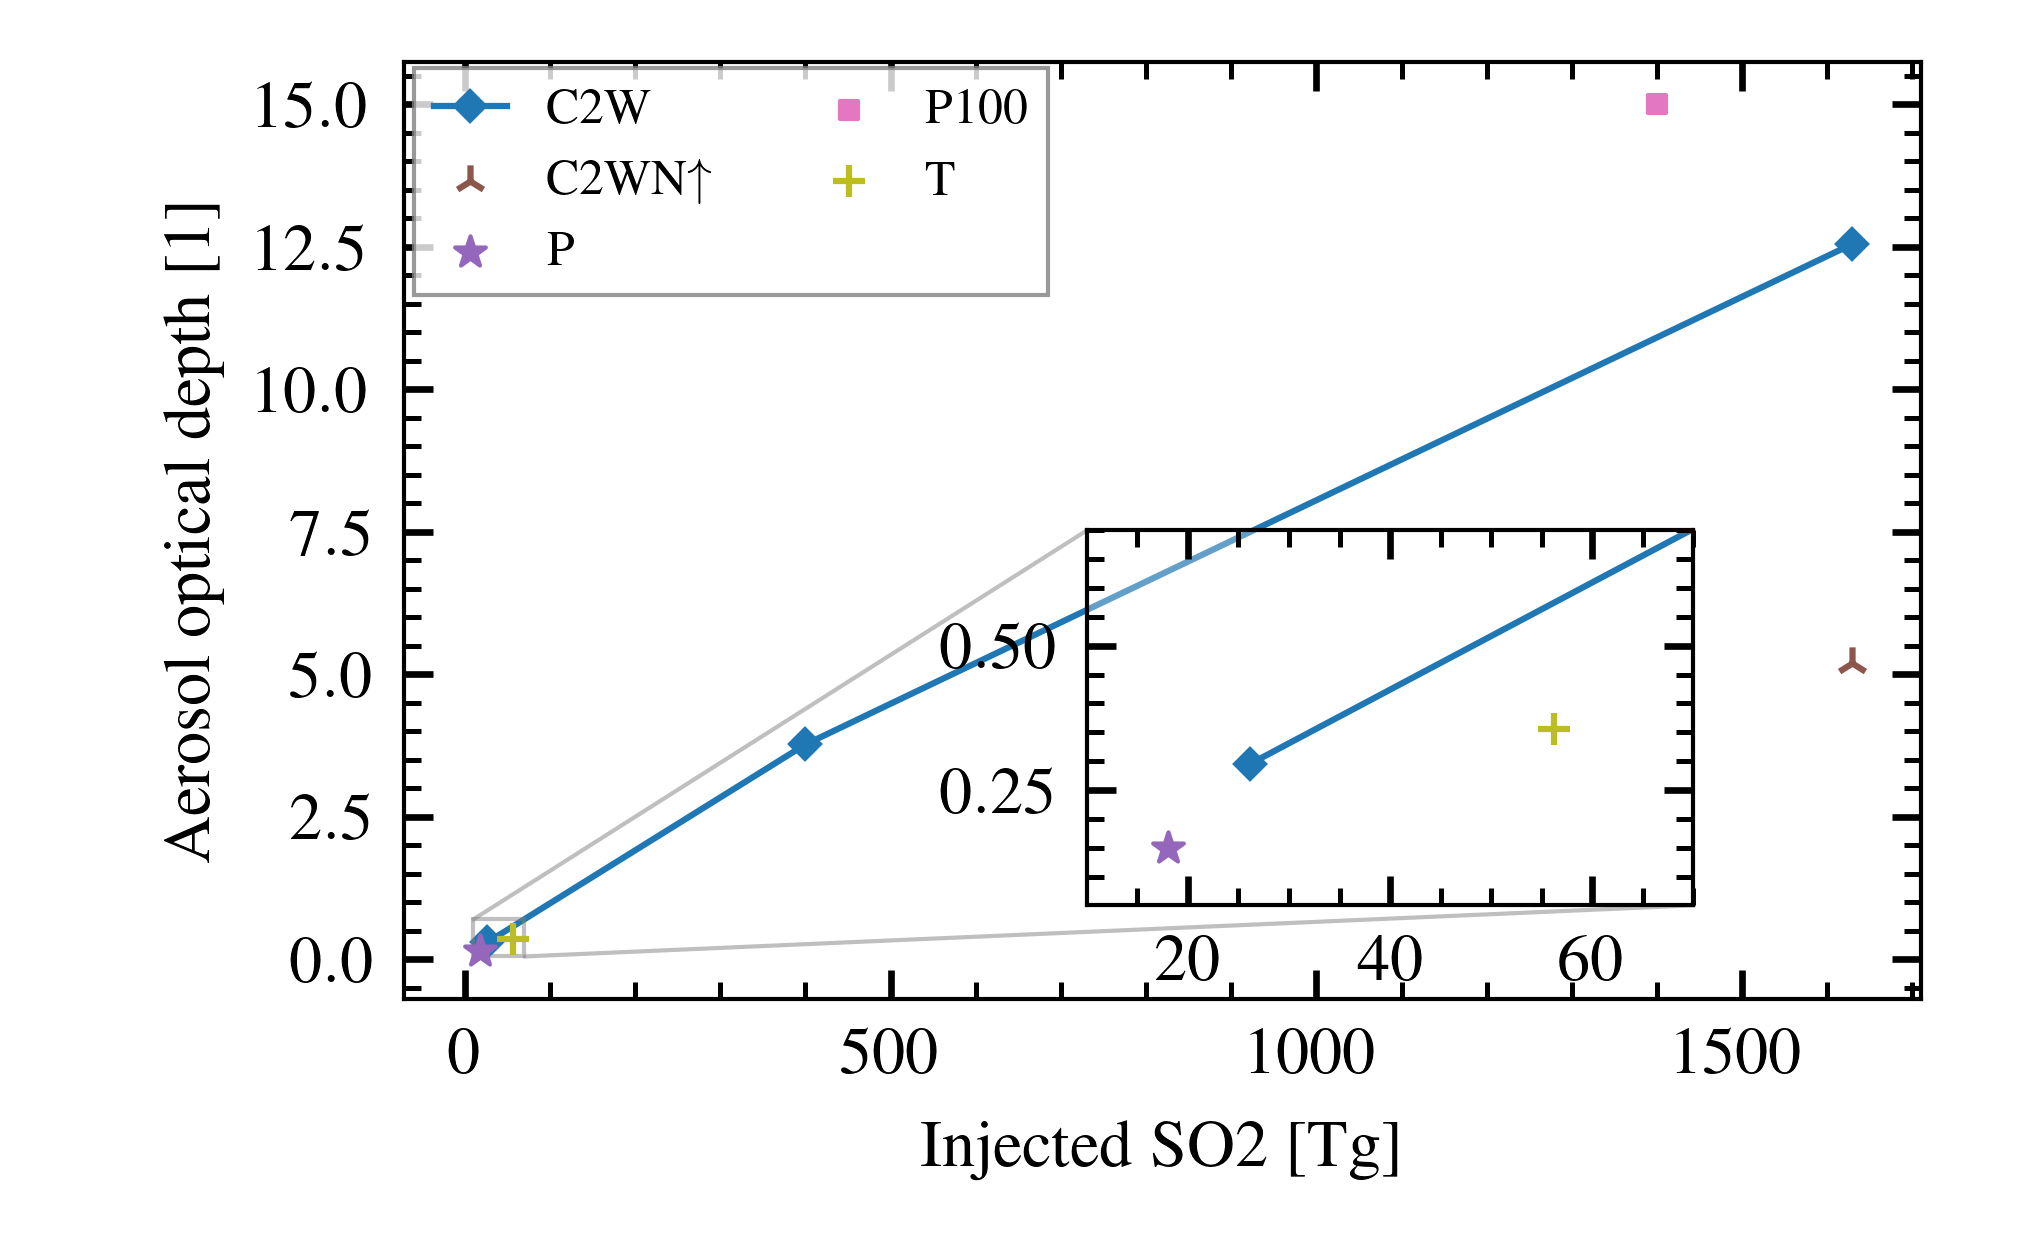
\includegraphics[width=0.95\linewidth]{figures/injection_vs_aod.png}
  \end{center}
  \caption{Injected \ce{SO2} versus \ac{aod}}%
  \label{fig:so2_vs_aod}
\end{figure}

With the almost linear relation between injected \ce{SO2} and \ac{aod}, we should expect
to see a similar plot for \iso{} versus \ac{rf} as for \ac{aod} versus \ac{rf}. \iso[I]
versus \ac{rf} is shown in \cref{fig:so2_vs_toa}, but where the absolute value of the
\ac{rf} is potted along the \( y \)-axis. Just as in \cref{fig:aod_vs_toa_full} we find
the \ac{cesm2} data points to be heavily damped in \ac{rf} as \iso{} increases. The same
effect can be seen in the data from \citet{ottobliesner2016} (labelled C1C, red points),
but here the \ac{rf} tend to bend off sooner, having a smaller \ac{rf} response to
\iso{} than the \ac{cesm2} data. The simulations used by \citet{ottobliesner2016} was
with \ac{cesm} as well, but version 1 (\ac{cesm1}) and with a low-top atmosphere
(\ac{cam5}). The difference in model complexity might therefore be the reason why the
\iso{} give weaker \ac{rf} response for \citet{ottobliesner2016} than what we find.

\begin{figure}[t]
  \begin{center}
    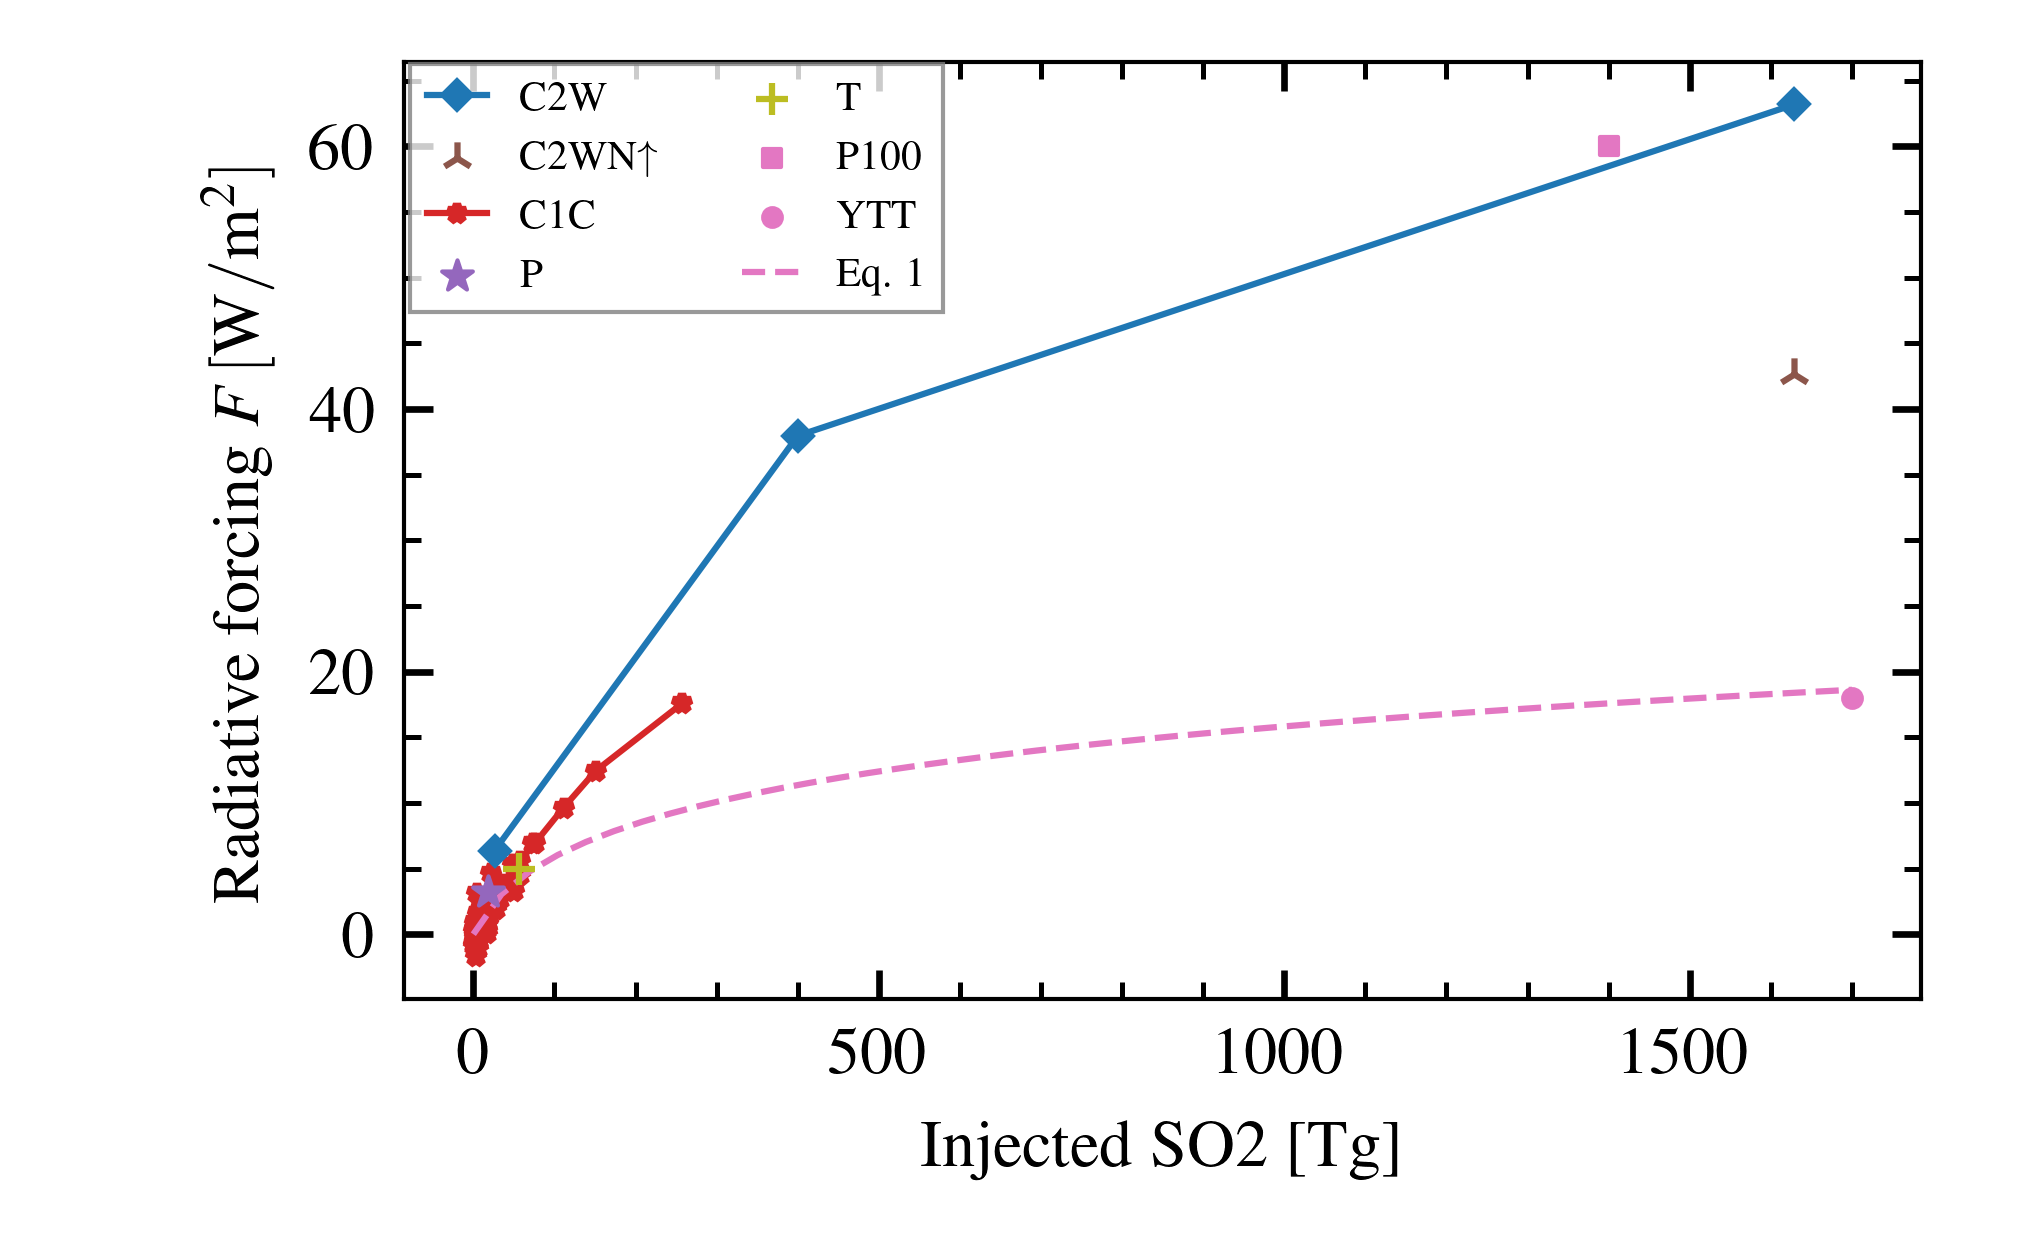
\includegraphics[width=0.95\linewidth]{figures/injection_vs_toa.png}
  \end{center}
  \caption{Injected \ce{SO2} versus \ac{rf} radiative imbalance}%
  \label{fig:so2_vs_toa}
\end{figure}

\Cref{fig:so2_vs_temp} show \iso{} versus temperature response. Just as in
\cref{fig:so2_vs_toa}, the data from the \ac{cesm2} simulations bend off, making the
temperature response less extreme for higher values of \iso. Again we see that the data
from the \ac{cesm1} simulations by \citet{ottobliesner2016} follow a different path than
the \ac{cesm2} data, with weaker temperature fluctuations for a given \iso{}, as one
would expect based on \cref{fig:so2_vs_toa}.

\begin{figure}[t]
  \begin{center}
    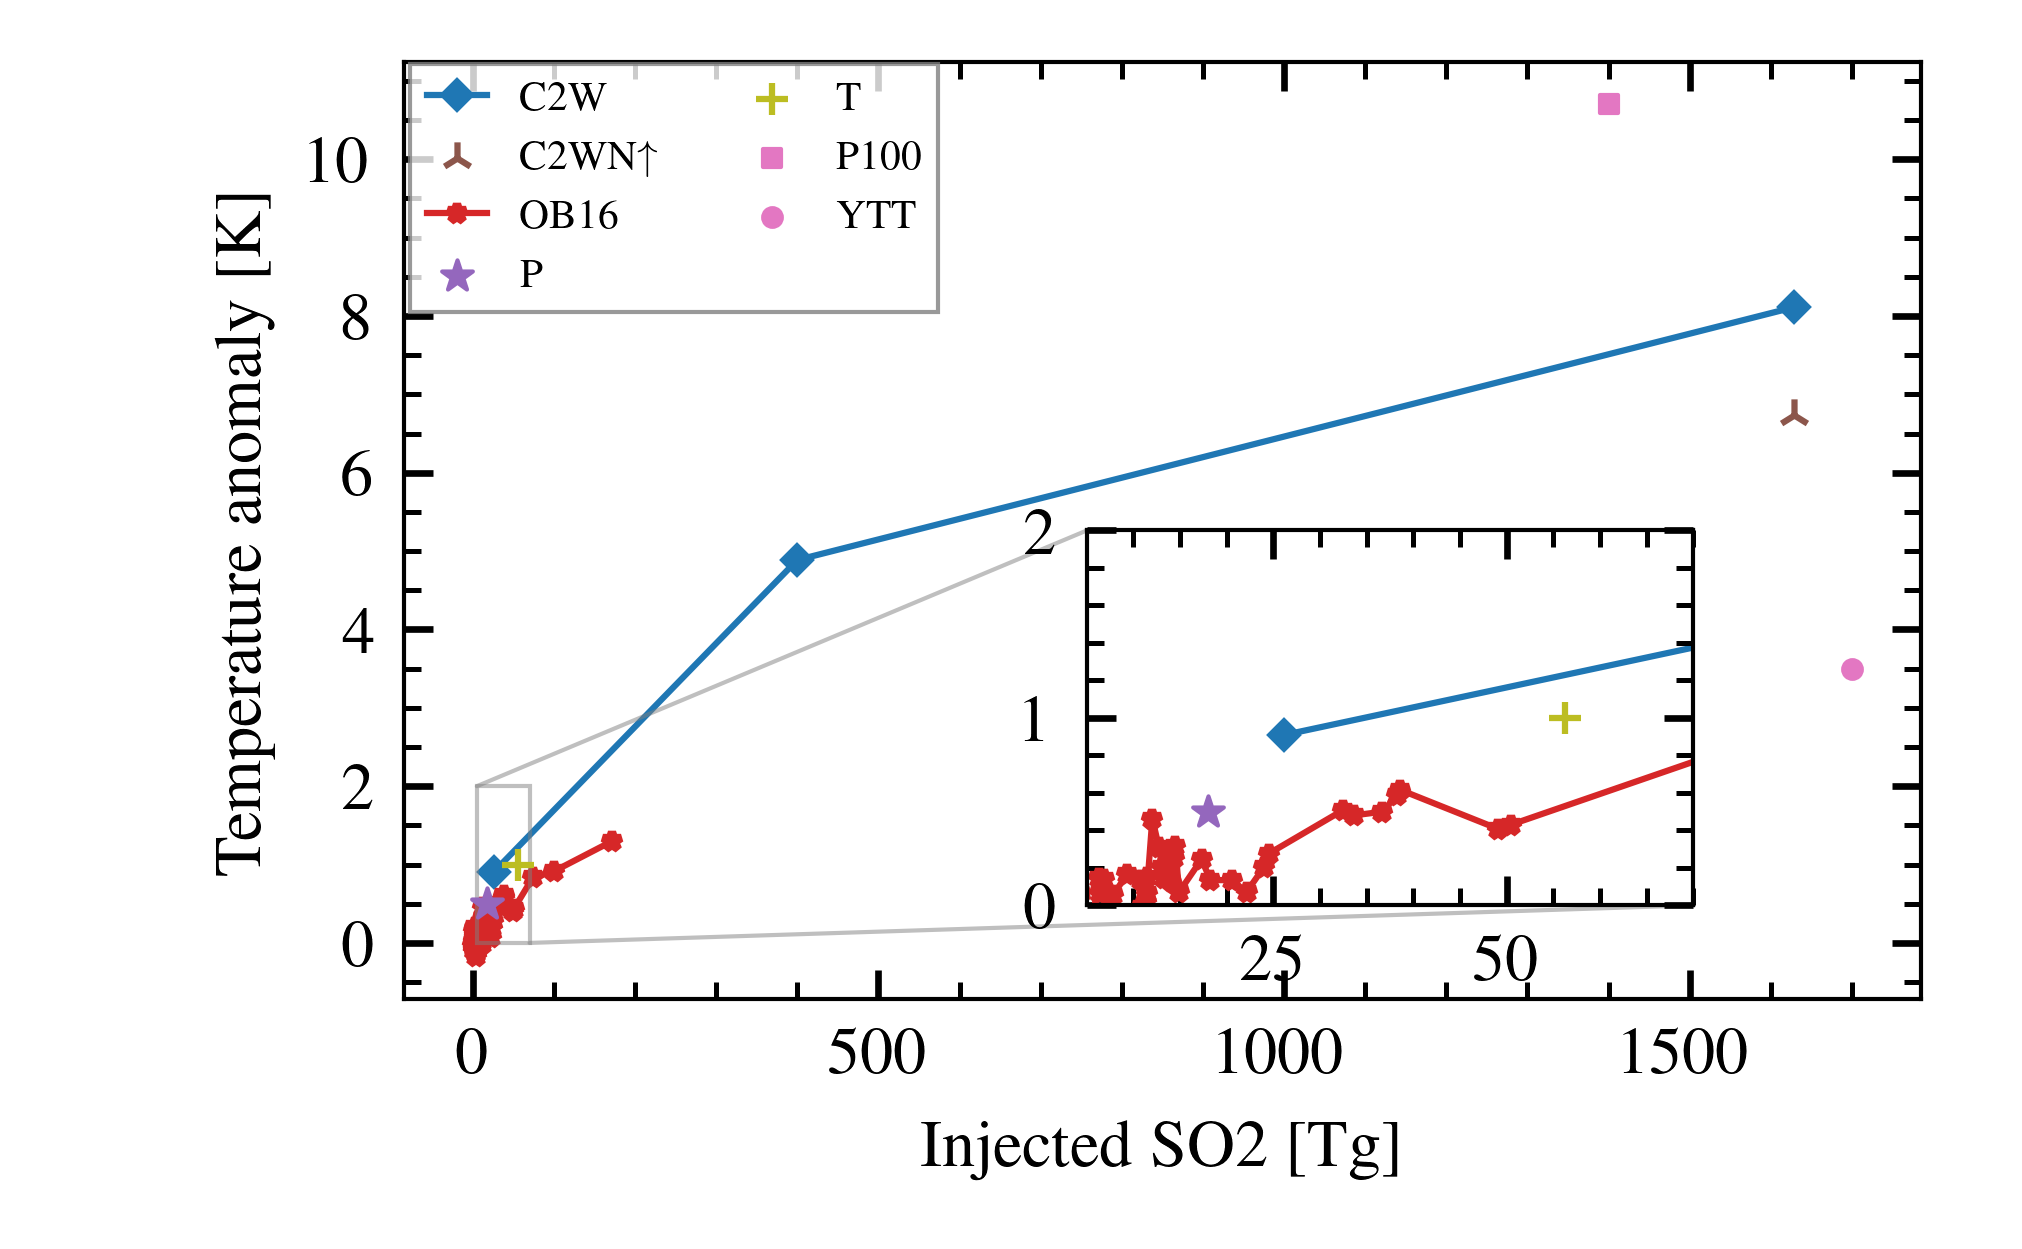
\includegraphics[width=0.95\linewidth]{figures/injection_vs_temperature.png}
  \end{center}
  \caption{Injected \ce{SO2} versus temperature}%
  \label{fig:so2_vs_temp}
\end{figure}

\Cref{fig:aod_vs_temp} should in the case of the \ac{cesm2} data points be very similar
in shape to the paths found in \cref{fig:so2_vs_temp} due to the close to linear
relationship found between \iso{} and \ac{aod} in \cref{fig:so2_vs_aod}. The
relationship between \ac{aod} and temperature is slightly more linear than what is the
case with \iso{} and temperature, but the tendency is still the same.

\begin{figure}[t]
  \centering
  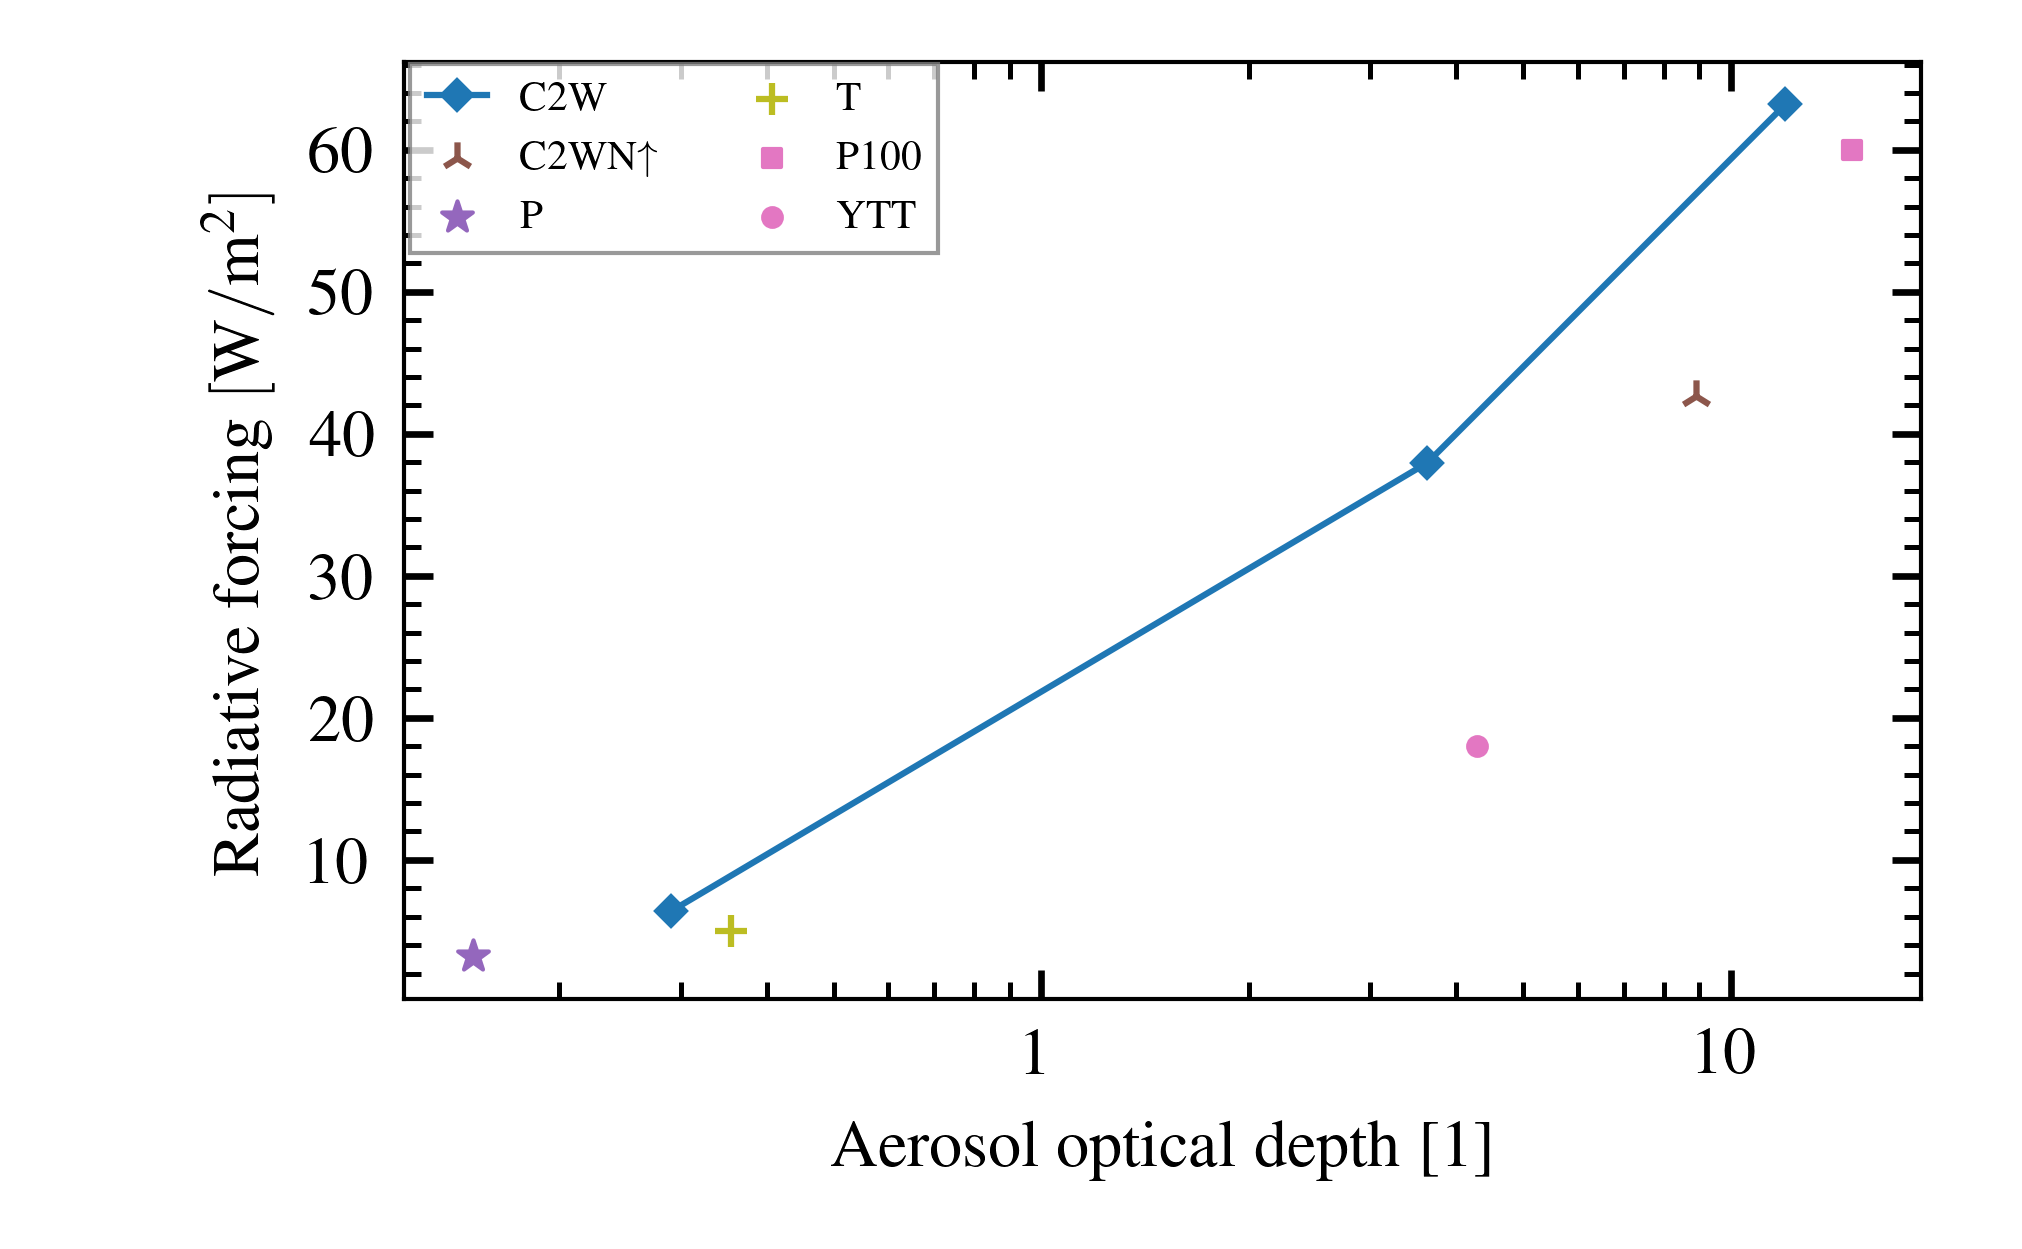
\includegraphics[width=0.95\linewidth]{figures/aod_vs_toa_logscale.png}
  \caption{\ac{aod} versus \ac{rf}}%
  \label{fig:aod_vs_toa_logscale}
\end{figure}

\begin{figure}[t]
  \begin{center}
    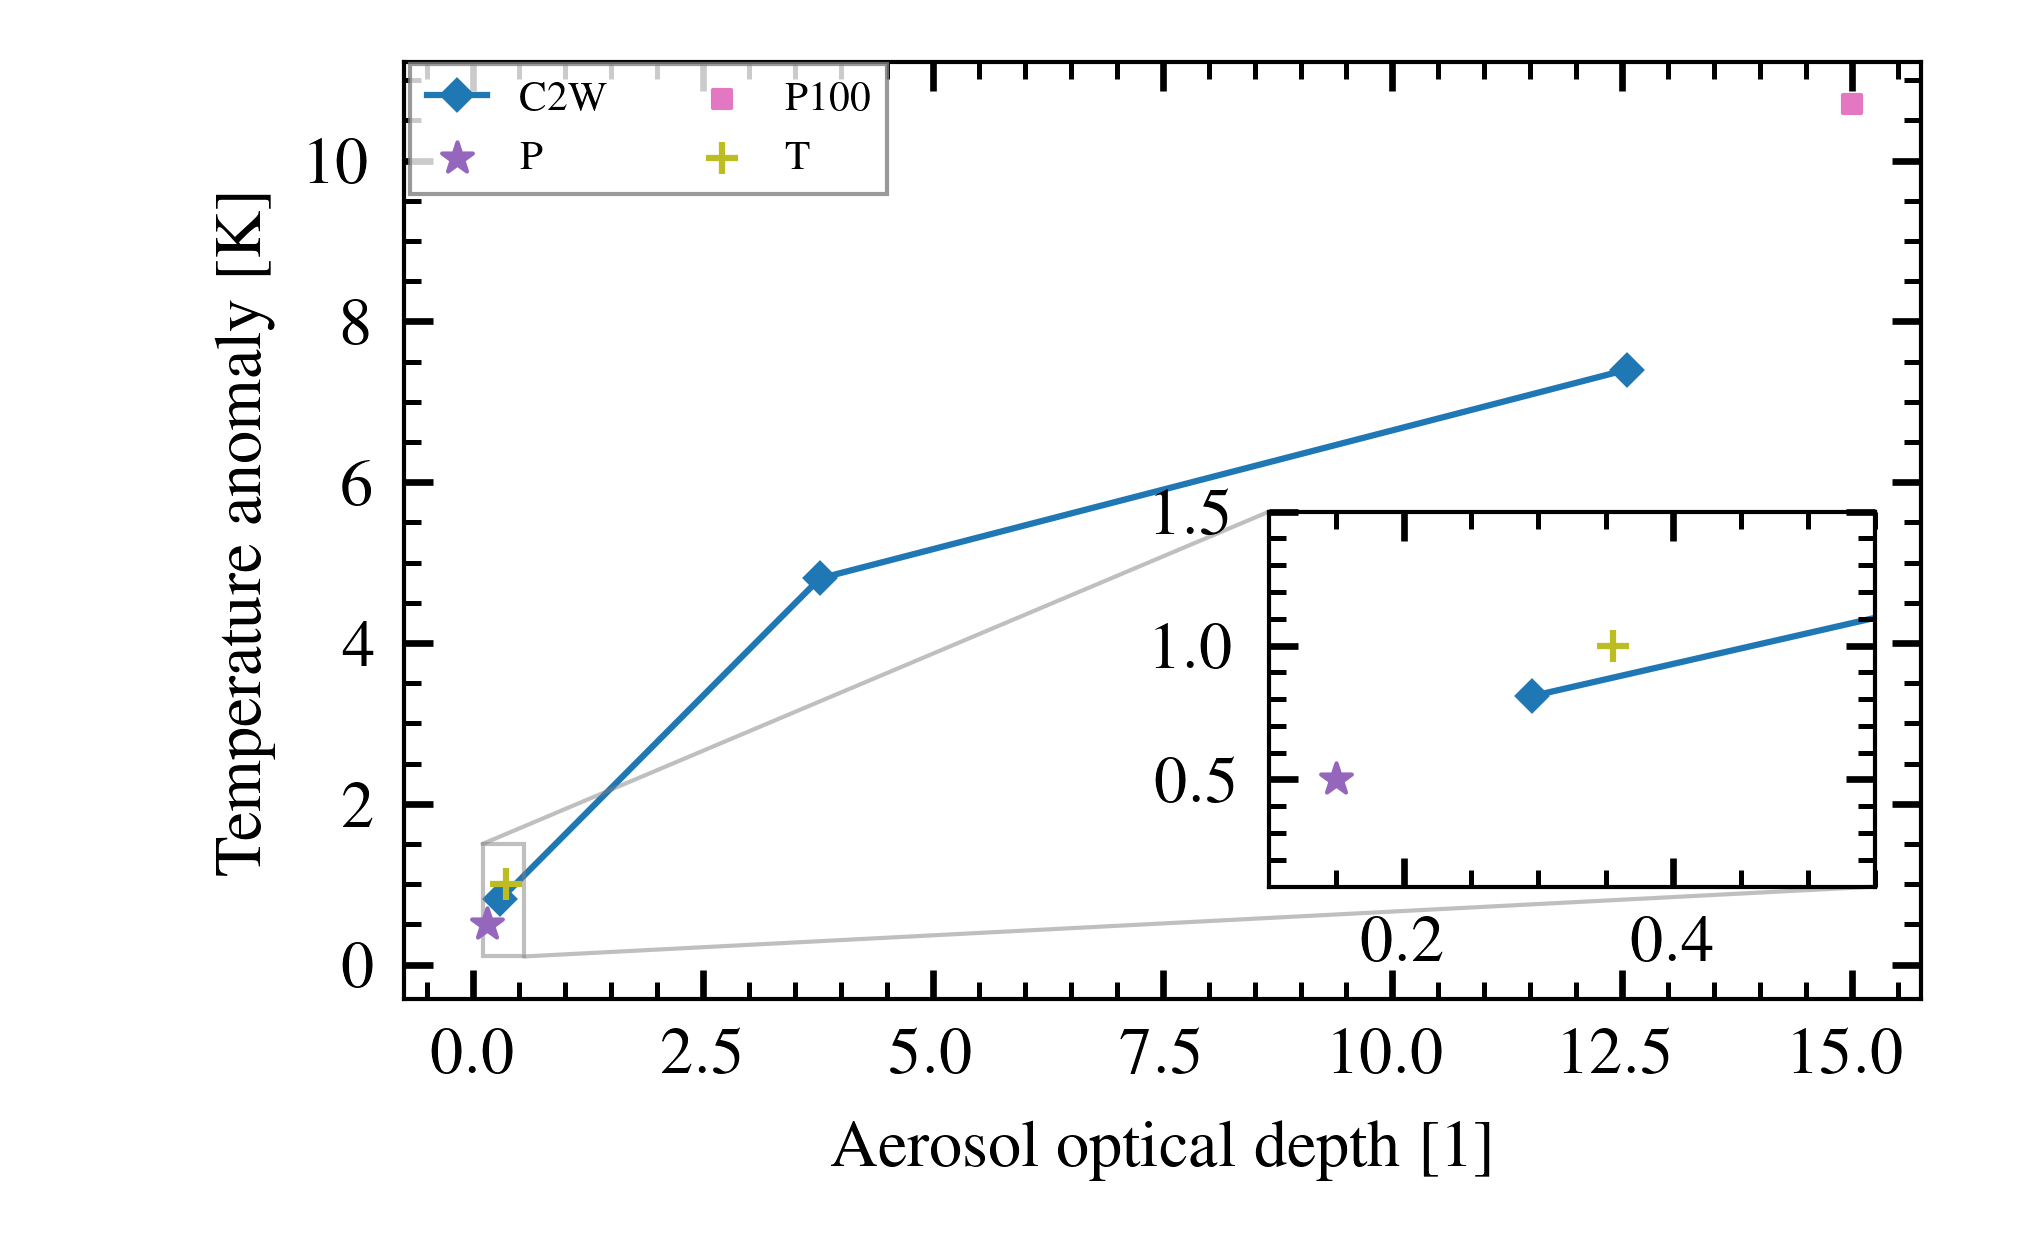
\includegraphics[width=0.95\linewidth]{figures/aod_vs_temperature.png}
  \end{center}
  \caption{\ac{aod} versus temperature}%
  \label{fig:aod_vs_temp}
\end{figure}

In \cref{fig:toa_vs_temp} we compare the \ac{rf} and temperature response. Both the
\ac{cesm2} data and the \ac{cesm1} from \citet{ottobliesner2016} show a close to linear
relationship between temperature and \ac{rf}, but where the \ac{cesm2} data seem to lead
to stronger temperature perturbations compared to \ac{cesm1}. However, the overlap in
data is not big, and the \ac{cesm2} data is too sparse to make strong conclusions, in
addition to the difference in model complexity.

While the \ac{p100} data have been comparable to the strong \ac{cesm2} data point in
both \ac{aod} and \ac{rf}, the temperature response reported by \citet{jones2005} is
much stronger than what our strongest eruption caused. Since \citet{jones2005} used the
\ac{aod} forcing from Mt. Pinatubo multiplied by one hundred, the shape during the whole
phase could be significantly different to what a super-eruption would create, even
though the peak is representable, as we have seen in \cref{fig:aod_arrays_normalized}
where the \ac{aod} shape differ as the eruption strength is increased. This might be
enough to cause a much stronger temperature perturbation. We also note that
\citet{timmreck2010} used a more realistic \ac{aod} forcing and obtained cooling that
was much smaller than \citet{jones2005}. \emph{(More on this in
  \cref{sec:discussion}\ref{sec:climate-sensitivity-estimate}.)}

\begin{figure}[t]
  \begin{center}
    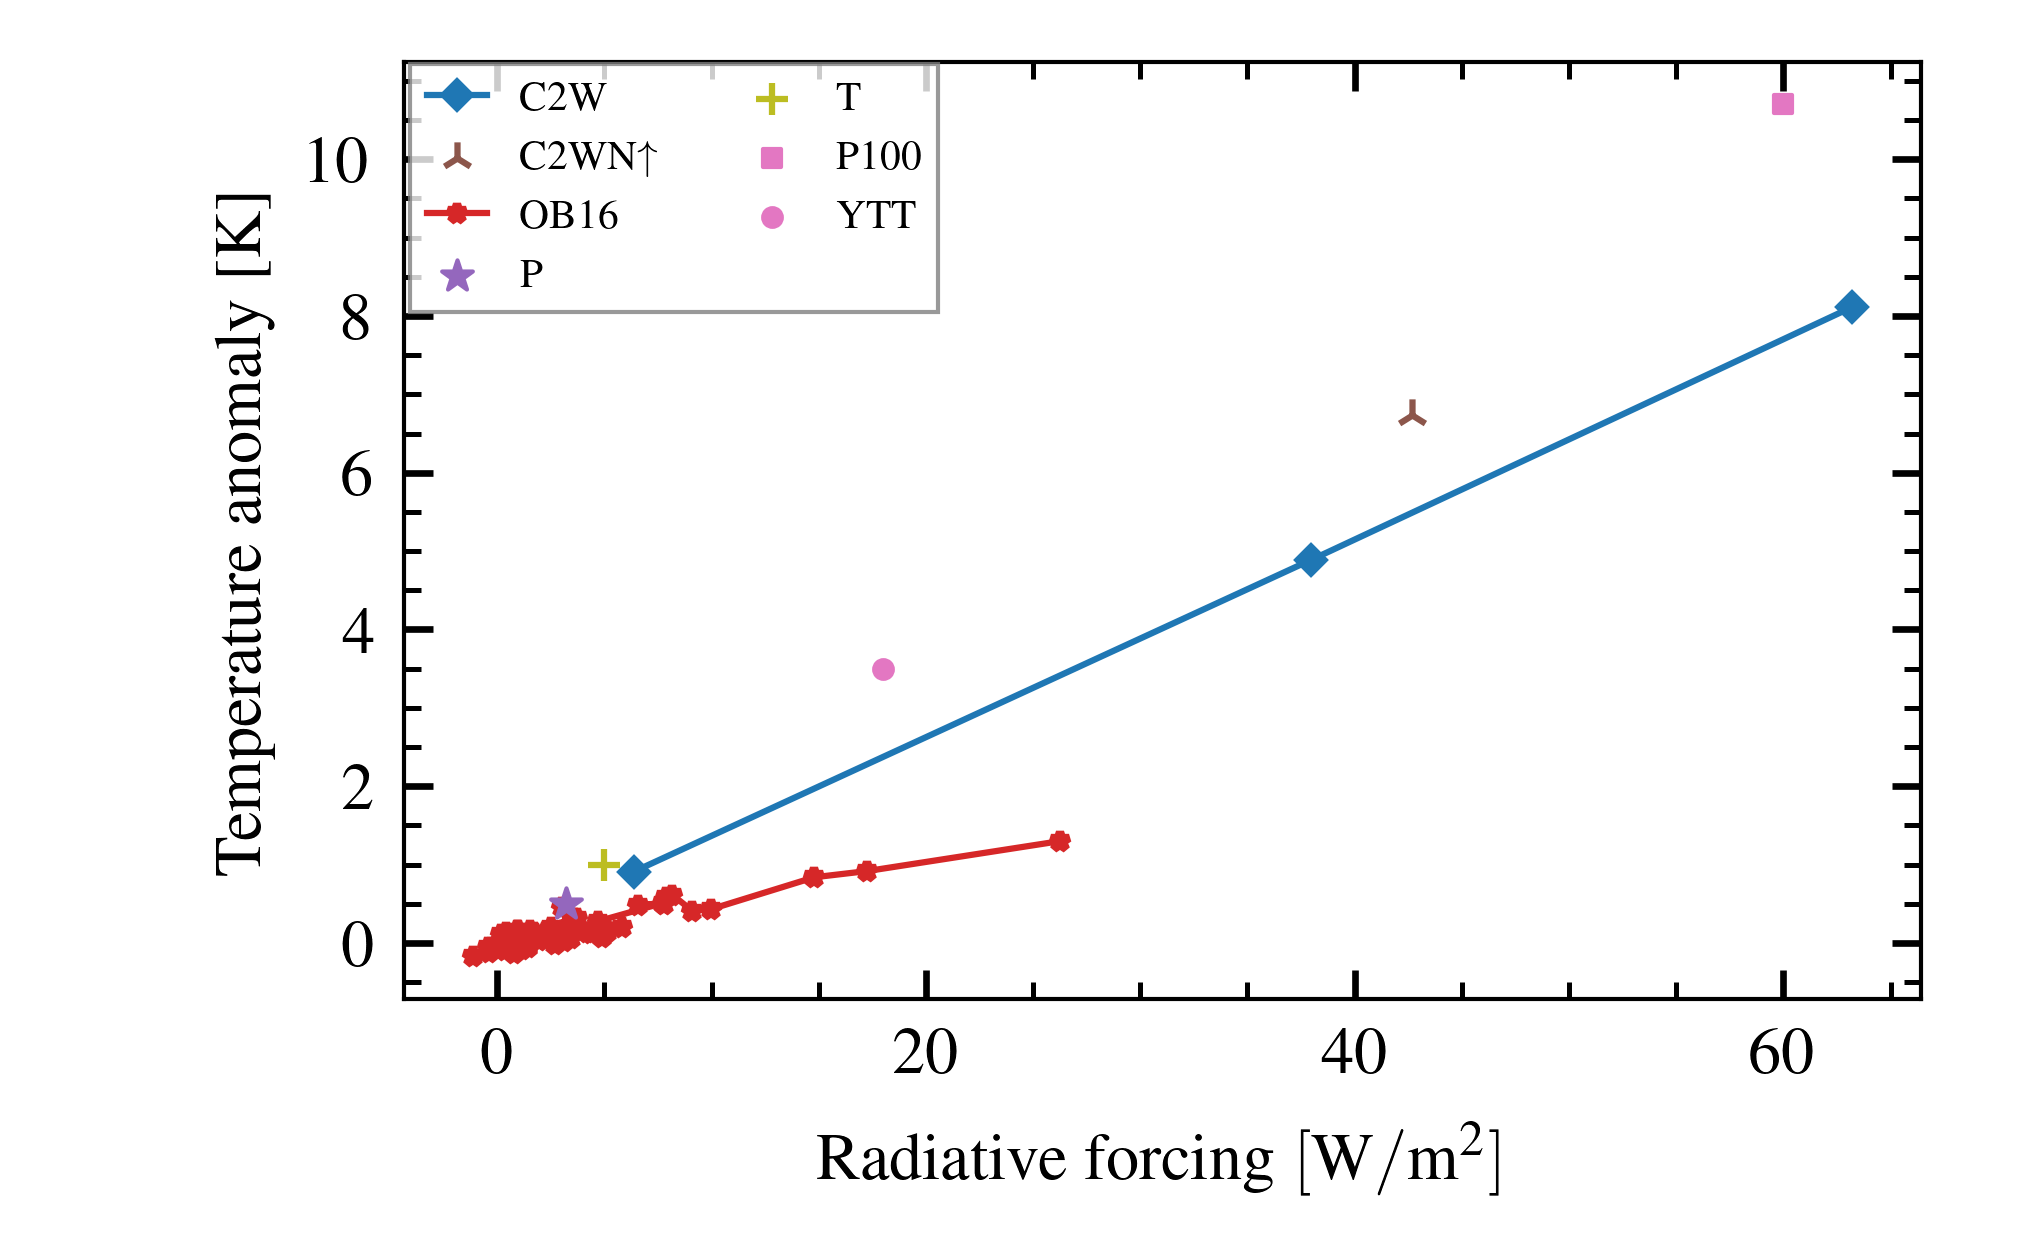
\includegraphics[width=0.95\linewidth]{figures/toa_vs_temperature.png}
  \end{center}
  \caption{\ac{rf} versus temperature}%
  \label{fig:toa_vs_temp}
\end{figure}

\section{Discussion}%
\label{sec:discussion}

\Cref{fig:aod_vs_toa_full,fig:aod_vs_toa_inset,fig:aod_vs_toa_avg_loop,fig:aod_vs_toa_avg_loop_scaled,fig:aod_vs_toa_avg_loop_ratio,fig:aod_vs_toa_avg_loop_ratio_scaled,fig:aod_vs_toa_logscale}
all show that as the \ac{aod} values are increased past \(\sim 0.5\), the scaling of
\(\sim -20\) no longer map to corresponding values of \ac{rf}. When looking at the
intermediate volcanic eruption with \(\SI{400}{\tera\gram}\) \iso{} there seem to be a
mostly linear relationship between the \ac{aod} and \ac{rf} values, with a slope of
approximately \(-10\). As for the largest eruption, scaling \ac{aod} by \(\sim-4\)
yields reasonable \ac{rf} values. From \cref{fig:so2_vs_aod} we have an almost linear
relation between \iso{} and \ac{aod}, and previous results indicate that larger
eruptions where more \ce{SO2} is injected creates larger aerosols which are less
effective at scattering radiation, making the cooling less efficient
\citep{english2013,timmreck2010,timmreck2018}. (\citet{timmreck2010} mention that for
very large eruptions, they look at Pinatubo and \ac{ytt}, \ce{OH} radicals are not
abundant enough which limit the \ce{SO2} oxidation. Originally in \citep{bekki1995}.)
The peak in \ac{aod} levels for the \ac{ytt} simulation appear six months after the peak
of Pinatubo (or a \ac{p100} scaling) in \citet{timmreck2010}, and at a much smaller
value, see their fig.\ 1c. \citet{timmreck2010} also obtained a peak \ac{rf} anomaly of
\(\SI{-18}{\watt\metre^{-2}}\) (\(7\)-\(8\) months after) compared to \citet{jones2005}
of \(\SI{-60}{\watt\metre^{-2}}\) (one year after). (\ac{rf} peak occurring prior to the
\ac{aod} peak is the same as I see with my simulations, especially with the larger
ones.)

From the smallest and the intermediate eruption sizes, there is an apparent roughly
linear relationship between \ac{aod} and \ac{rf}. Only when inspecting the data
generated from the largest eruption at \(\SI{1629}{\tera\gram}\) of \iso{} can we see
that it initially follow approximately the same path as the intermediate, before it
continues on a much less steep path. Yet, the shape that the two eruptions draw is very
similar when scaled, suggesting that the intermediate also do follow a loop and that it
is not just noise that causes the spread. That is, there appear to be a
time-after-eruption dependency on the ratio between \ac{aod} and \ac{rf}.
\citet{marshall2020} discuss a similar feature they find when looking at \ac{aod} and
\ac{rf}, but there, the efficiency increases from year 1 to year 2, while here
efficiency decreases with time. \citet{marshall2020} explain that this is due to the
time it takes for the aerosols to spread which affects the global albedo and in turn the
\ac{rf}, while the \ac{aod} being less affected by the aerosols spreading.

An attempt to reason for the decrease in efficiency being more likely: smaller eruptions
and estimates from them give an \ac{rf} to \ac{aod} that is quite steep, while larger
eruptions (or values of \iso{} in the atmosphere as used in \citet{niemeier2015}) result
in estimates that are smaller in magnitude (\(\sim-20\) versus \(\sim-10\) to
\(\sim-4\), \cref{fig:aod_vs_toa_avg_loop_ratio}). It has been shown that that
efficiency decrease as the injection rate increase \citep{niemeier2017}, related to the
\ac{qbo}, and that large volcanic eruptions result in larger aerosol particle sizes
which result in decreasing cooling efficiency per \iso{} \citep{english2013,
  timmreck2018}. Can this be used to reason that the efficiency is initially high, then
decreasing? Perhaps several and competing effects (albedo, \ac{qbo}, particle size,
growth \& sedimentation phases)?

Large compared to small eruptions:

\begin{enumerate}
  \item \ce{SO2} oxidises more slowly due to lack of \ce{OH}, which delays the peak \ac{aod}
        level
  \item Aerosols grow to larger radii, which makes them less efficient at scattering radiation,
        so you have less cooling for the same amount of \iso{}
  \item Larger aerosols stay for a shorter time due to being heavier (and other causes? Verify.)
  \item \ac{rf} plot (\cref{fig:toa_arrays_normalized}) show very similar shape when they are
        scaled; smaller eruptions are more efficient throughout, but especially in the early
        phase, why? (\Cref{fig:aod_vs_toa_avg_loop_ratio}.)
\end{enumerate}

\subsection{Climate sensitivity estimate}%
\label{sec:climate-sensitivity-estimate}

The climate feedback (response) parameter is estimated by \citet{jones2005} to be
\(\alpha \simeq \SI{4}{\watt\metre^{-2}\kelvin^{-1}}\) (Still not sure how they do this,
you need constant forcing, no?), which was more than twice (and half the sensitivity,
[since this is the reciprocal?]) of what \citet{gregory2016} obtained in their
simulations using Pinatubo in the HadCM3 climate model. (they used a step volcanic
forcing simulation to obtain their estimate).

Instead of estimating \(\alpha \), we focus our attention to the climate resistance
\(\rho \), and the \ac{tcrp} \(1/\rho\) (where \(\mathrm{TCR}=F_{2\times}\times
\mathrm{TCRP}\) is the transient climate sensitivity). Even though the forcing from
volcanic eruptions last only for about a year, which is too short for the timescales at
which \(F=\rho T\) is valid \citep{gregory2016}, we might get around this by using a
time-integral form introduced by \citet{merlis2014}
\begin{equation}
  \int_0^{\tau}F \mathrm{d}t=\rho\int_{0}^{\tau}T \mathrm{d}t
\end{equation}
\begin{equation}
  \rho=\frac{\int_0^{\tau}F \mathrm{d}t}{\int_{0}^{\tau}T \mathrm{d}t}.
  \label{eq:climate-resistance}
\end{equation}
%
If the upper bound of the integral, \(\tau \), is big enough such that the upper ocean
heat capacity is the same at \(t=0\) and \(t=\tau \), then this agrees with \(F=\rho T\)
\citep{gregory2016} (\citet{merlis2014} used \(\tau =\SI{15}{\mathrm{y}}\)). We also
note that the climate resistance and the climate feedback parameter are related to the
ocean heat uptake efficiency \(\kappa \) through \(\rho =\alpha +\kappa \).

When computing the trapezoidal integral of the forcing and temperature before finding
the ratio, the three main simulation types (four in each ensemble) give estimated
\ac{tcrp} of \(3.3\), \(3.12\) and \(2.91\), shown in \cref{tab:trcp}. This is not the
same as the climate feedback parameter \citet{jones2005} estimated, but as both \(\alpha
\) and \(\kappa \) are positive, and our estimates of \(\rho (=\alpha +\kappa) \) are
all less than the \citet{jones2005} estimate of \(\alpha \simeq
\SI{4}{\watt\metre^{-2}\kelvin^{-1}}\), we conclude that the climate feedback parameter
related to the simulations done here is significantly less than what \citet{jones2005}
got.

\begin{table}
  \centering
  \caption{Estimated climate resistance and \ac{tcrp} by use of the method outlined by
    \citet{merlis2014}. Estimates are based on ensembles with four members, and where
    \(\tau =\SI{9}{\mathrm{y}}\) in \cref{eq:climate-resistance}}%
  \label{tab:trcp}
  \begin{tabular}{ccc}
    Simulation type & \(\rho [\si{\watt\metre^{-2}\kelvin^{-1}}]\) & \(1/\rho\)         \\
    Small           & \(\num{3.3(9)}\)                             & \(\num{0.32(7)}\)  \\
    Intermediate    & \(\num{3.12(9)}\)                            & \(\num{0.321(9)}\) \\
    Large           & \(\num{2.91(8)}\)                            & \(\num{0.34(1)}\)  \\
  \end{tabular}
\end{table}

\section{Conclusions}

% NOTE: what we have done, future work, going back to points from introduction

In this paper we considered three large to super-volcano sized eruptions.

\clearpage

To-do:

\begin{itemize}
  \item[\lbrack{}x\rbrack{}] Create an estimate of climate sensitivity from volcanoes.
    \citet{gregory2016} talks about what they got in \citet{jones2005}, so maybe comparing
    is worthwhile. \emph{Did find the \ac{tcrp} according to \citet{merlis2014}, which gives
      some ground for comparison, but the climate feedback parameter is missing.}
  \item[\lbrack{}x\rbrack{}] Create plots also using the \(1-\mathrm{e}^{-\mathrm{AOD}}\), like
    in Marshall et al.\ (2020). \emph{For data greater than 1, the scaling squishes it a
      lot.}
\end{itemize}

\section*{Climate sensitivity estimate}

From \citet{gregory2016}: ``The peak forcing was about \(\SI{-60}{\watt\metre^{-2}}\),
only \(20\) times greater than Pinatubo, and the climate feedback parameter \(\alpha
\simeq \SI{4}{\watt\metre^{-2}\kelvin^{-1}}\), more than twice the value (half the
climate sensitivity parameter [which is the reciprocal?]) that we found for Pinatubo in
HadCM3.''

\(1/\rho \) is the ``transient climate response parameter'' (where
\(\mathrm{TCR}=F_{2\times}\times \mathrm{TCRP}\) is the transient climate sensitivity),
where \(\rho \) is a climate resistance obtained from \(F(t)=\rho T(t)\), where the
forcing increase at a roughly constant rate.

The climate feedback parameter \(\alpha\) and the ocean heat uptake efficiency
\(\kappa\) are both positive, and \(\rho =\alpha +\kappa \). In this picture, \(T\) is a
surface skin temperature, with negligible thermal inertia, determined by the Earth
energy balance \(F=N+\alpha T\), where \(N\) is the net downward radiative heat flux at
the top of the atmosphere, and \(N=\kappa T\) if we neglect heat storage other than in
the ocean. We call \(F=\rho T\) the ``zero-layer model''.

``For volcanic forcing which is large in magnitude for only a year or two, the
\ac{tcrp} and the zero-layer model are therefore not applicable.'' They
\citep{gregory2016} use an abruptPin simulation to estimate the climate feedback
parameter \(\alpha \) for volcanic forcing in comparison to forcing from for example
\(4\times \ce{CO2}\). Possible to use method outlined by \citet{merlis2014}? That is,

\citet{gregory2016} use \(F=N+\alpha T\) while \citet{jones2005} use \(Q=N+\lambda
\Delta T\) to describe the same thing. Also, \citet{merlis2014} is using
\(\tilde{\beta}=\rho\), \(\beta =\alpha =\lambda \), \(\gamma =\kappa \) and
\(\mathcal{F}=F\). See \cref{tab:symbol-comparison}.

\begin{table}
  \centering
  \caption{For my own convenience, a comparison table comprising symbols used across
    the papers \citet{gregory2016} (G16), \citet{merlis2014} (M14) and \citet{jones2005}
    (J05). They all use \(T\) for the temperature and \(N\) for the net downward radiative
    heat flux at \ac{toa}}%
  \label{tab:symbol-comparison}
  \begin{tabular}{cccc}
    Name                         & G16         & M14                & J05          \\
    Forcing                      & \(F\)       & \(\mathcal{F}\)    & \(Q\)        \\
    Climate feedback parameter   & \(\alpha \) & \(\beta \)         & \(\lambda \) \\
    Climate resistance           & \(\rho \)   & \(\tilde{\beta }\) & \(-\)        \\
    Ocean heat uptake efficiency & \(\kappa \) & \(\gamma \)        & \(-\)        \\
  \end{tabular}
\end{table}

\clearpage

% %%%%%%%%%%%%%%%%%%%%%%%%%%%%%%%%%%%%%%%%%%%%%%%%%%%%%%%%%%%%%%%%%%%%%%%%%%%%%%%%%%%%%%
% ACKNOWLEDGMENTS
% %%%%%%%%%%%%%%%%%%%%%%%%%%%%%%%%%%%%%%%%%%%%%%%%%%%%%%%%%%%%%%%%%%%%%%%%%%%%%%%%%%%%%%
% \acknowledgments

% Keep acknowledgments (note correct spelling: no ``e'' between the ``g'' and ``m'') as
% brief as possible. In general, acknowledge only direct help in writing or research.
% Financial support (e.g. grant numbers) for the work done, for an author, or for the
% laboratory where the work was performed is best acknowledged here rather than as
% footnotes to the title or to an author's name. Contribution numbers (if the work has
% been published by the author's institution or organization) should be included as
% footnotes on the title page, not in the acknowledgments.

% %%%%%%%%%%%%%%%%%%%%%%%%%%%%%%%%%%%%%%%%%%%%%%%%%%%%%%%%%%%%%%%%%%%%%%%%%%%%%%%%%%%%%%
% DATA AVAILABILITY STATEMENT
% %%%%%%%%%%%%%%%%%%%%%%%%%%%%%%%%%%%%%%%%%%%%%%%%%%%%%%%%%%%%%%%%%%%%%%%%%%%%%%%%%%%%%%
% \datastatement

% The data availability statement is where authors should describe how the data
% underlying the findings within the article can be accessed and reused. Authors should
% attempt to provide unrestricted access to all data and materials underlying reported
% findings. If data access is restricted, authors must mention this in the statement.

% %%%%%%%%%%%%%%%%%%%%%%%%%%%%%%%%%%%%%%%%%%%%%%%%%%%%%%%%%%%%%%%%%%%%%%%%%%%%%%%%%%%%%%
% APPENDIXES
% %%%%%%%%%%%%%%%%%%%%%%%%%%%%%%%%%%%%%%%%%%%%%%%%%%%%%%%%%%%%%%%%%%%%%%%%%%%%%%%%%%%%%%
%
% Use \appendix if there is only one appendix.
% \appendix

% Use \appendix[A], \appendix[B], if you have multiple appendixes.
% \appendix[A]

% Appendix title is necessary! For appendix title:
% \appendixtitle{}

% Appendix section numbering (note, skip \section and begin with \subsection)
% \subsection{First primary heading}

% \subsubsection{First secondary heading}

% \paragraph{First tertiary heading}

% Important!
% \appendcaption{<appendix letter and number>}{<caption>}
% must be used for figures and tables in appendixes, e.g.
%
% \begin{figure}
% \noindent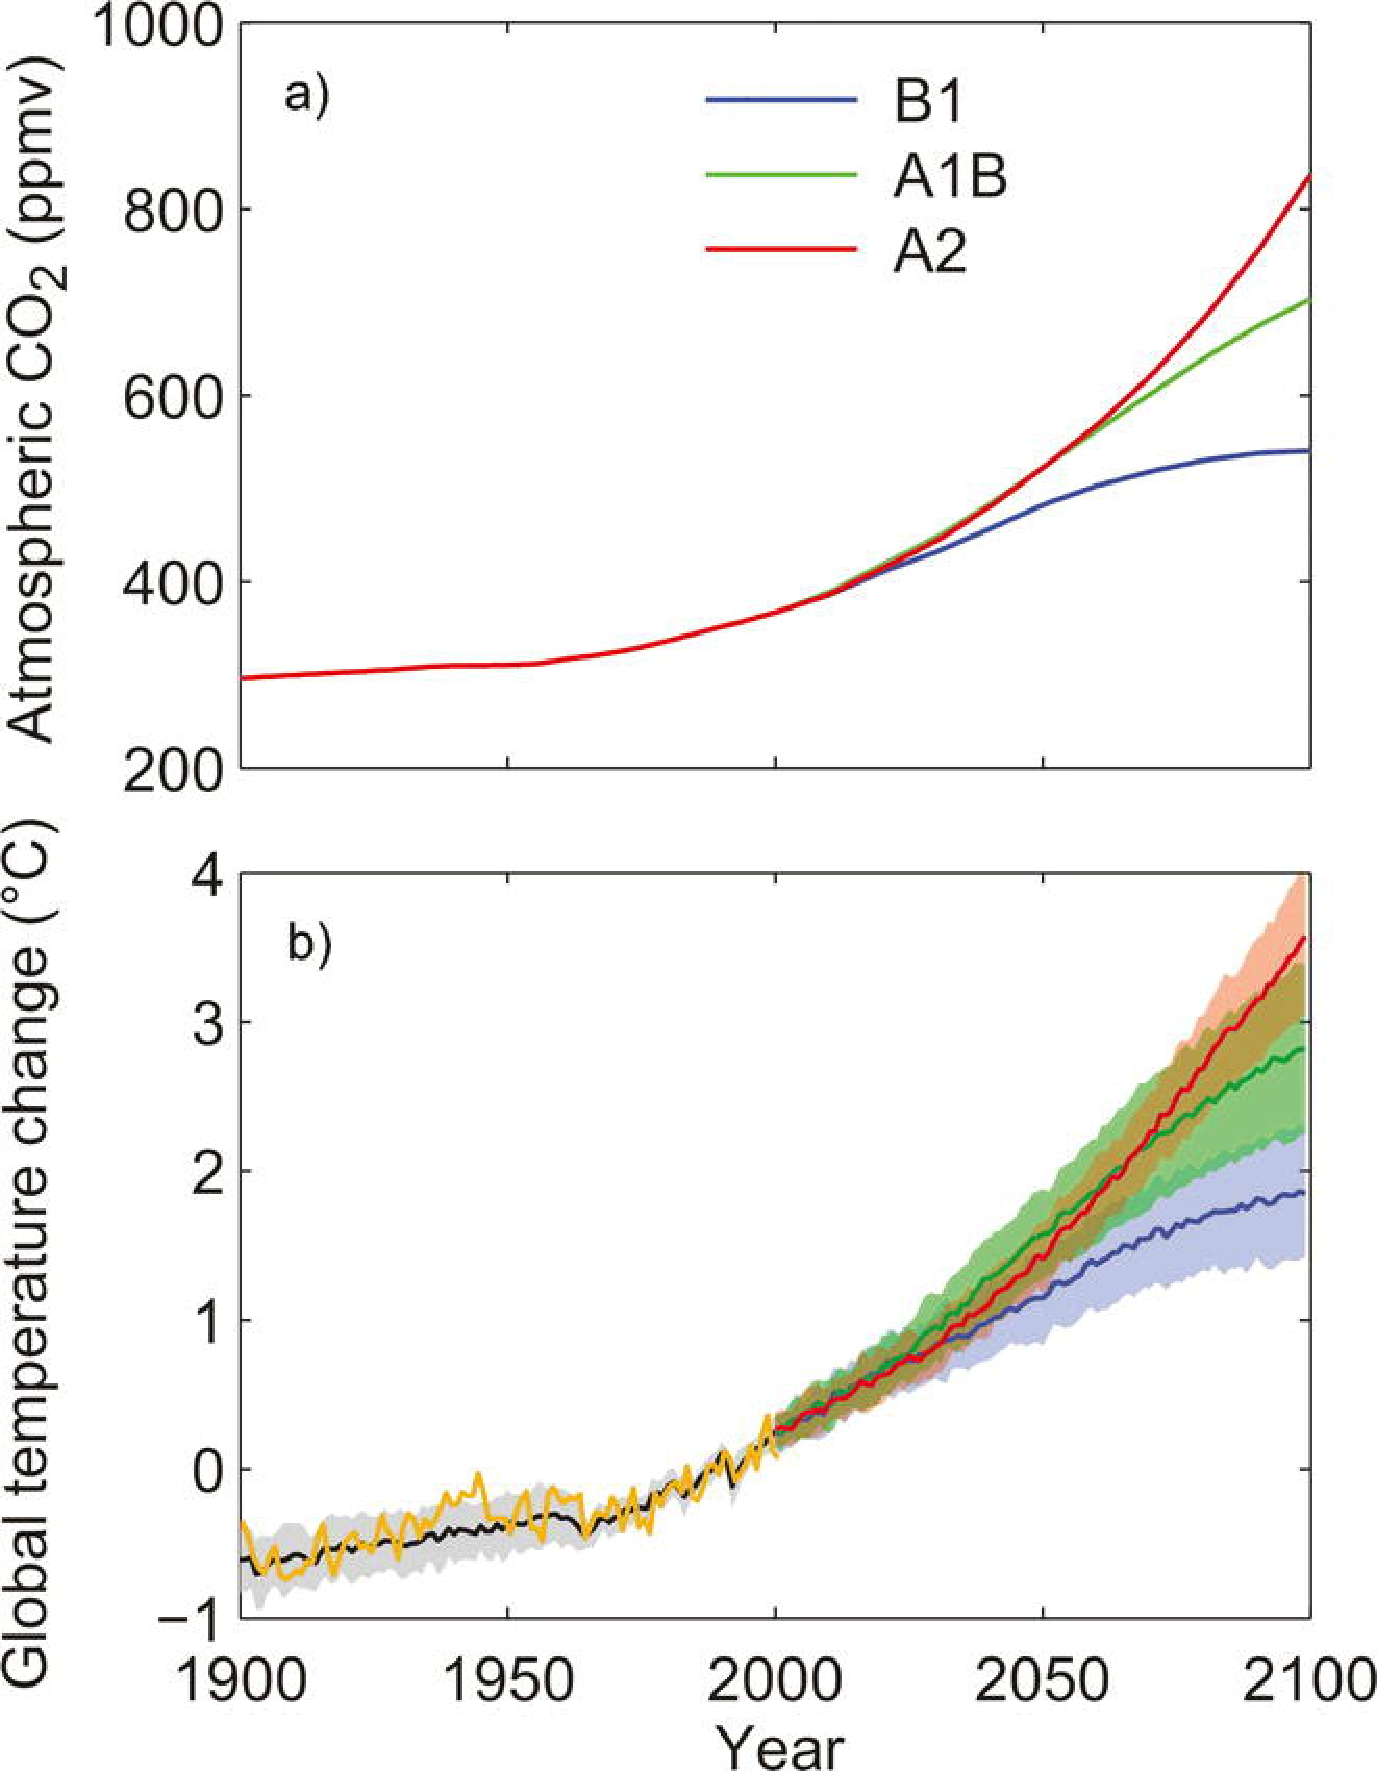
\includegraphics[width=19pc,angle=0]{figure01.pdf}\\
% \appendcaption{A1}{Caption here.}
% \end{figure}
%
% All appendix figures/tables should be placed in order AFTER the main figures/tables,
% i.e., tables, appendix tables, figures, appendix figures.
%
% %%%%%%%%%%%%%%%%%%%%%%%%%%%%%%%%%%%%%%%%%%%%%%%%%%%%%%%%%%%%%%%%%%%%%%%%%%%%%%%%%%%%%%
% REFERENCES
% %%%%%%%%%%%%%%%%%%%%%%%%%%%%%%%%%%%%%%%%%%%%%%%%%%%%%%%%%%%%%%%%%%%%%%%%%%%%%%%%%%%%%%
% Make your BibTeX bibliography by using these commands:
\bibliographystyle{ametsoc2014} \bibliography{references} \clearpage
\printglossary[type=\acronymtype,title=List of Acronyms]
% %%%%%%%%%%%%%%%%%%%%%%%%%%%%%%%%%%%%%%%%%%%%%%%%%%%%%%%%%%%%%%%%%%%%%%%%%%%%%%%%%%%%%%
% TABLES
% %%%%%%%%%%%%%%%%%%%%%%%%%%%%%%%%%%%%%%%%%%%%%%%%%%%%%%%%%%%%%%%%%%%%%%%%%%%%%%%%%%%%%%
% Enter tables at the end of the document, before figures.
%
% \begin{table}[t]
%   \caption{This is a sample table caption and table layout.  Enter as many tables as
%     necessary at the end of your manuscript. Table from Lorenz (1963).}\label{t1}
%   \begin{center}
%     \begin{tabular}{ccccrrcrc}
%       \hline\hline
%       $N$  & $X$  & $Y$  & $Z$  \\
%       \hline
%       0000 & 0000 & 0010 & 0000 \\
%       0005 & 0004 & 0012 & 0000 \\
%       0010 & 0009 & 0020 & 0000 \\
%       0015 & 0016 & 0036 & 0002 \\
%       0020 & 0030 & 0066 & 0007 \\
%       0025 & 0054 & 0115 & 0024 \\
%       \hline
%     \end{tabular}
%   \end{center}
% \end{table}

% %%%%%%%%%%%%%%%%%%%%%%%%%%%%%%%%%%%%%%%%%%%%%%%%%%%%%%%%%%%%%%%%%%%%%%%%%%%%%%%%%%%%%%
% FIGURES
% %%%%%%%%%%%%%%%%%%%%%%%%%%%%%%%%%%%%%%%%%%%%%%%%%%%%%%%%%%%%%%%%%%%%%%%%%%%%%%%%%%%%%%
% Enter figures at the end of the document, after tables.
%
% \begin{figure}[t]
%   \noindent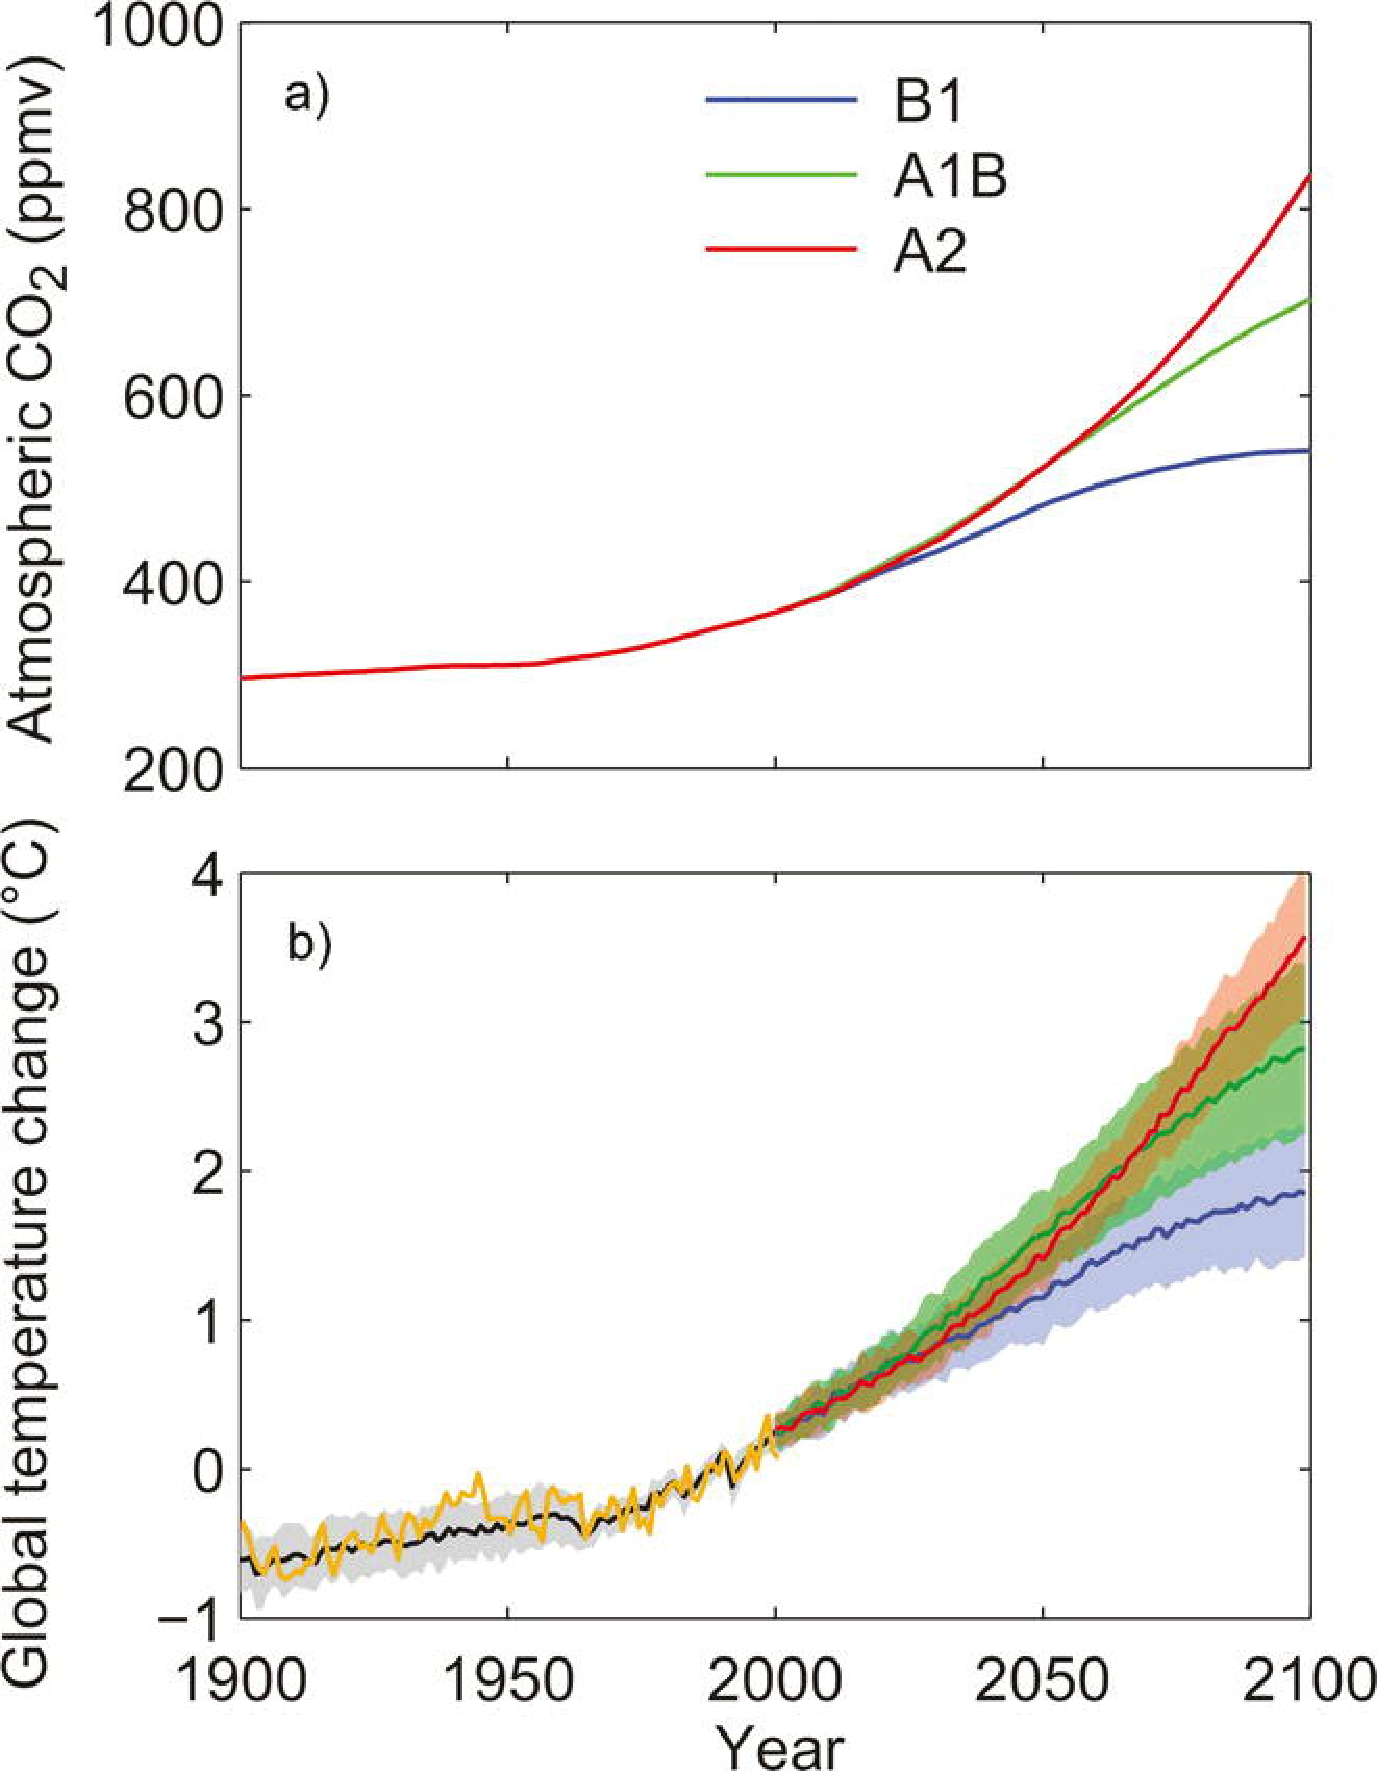
\includegraphics[width=19pc,angle=0]{figure01.pdf}\\
%   \caption{Enter the caption for your figure here.  Repeat as
%     necessary for each of your figures. Figure from \protect\cite{Knutti2008}.}\label{f1}
% \end{figure}

\begin{acronym}[AODVISstdn]
  % General
  \acro{aodm}[AODVISstdn]{``stratospheric aerosol optical depth 550 nm day night''}

  \acro{aod}[AOD]{(stratospheric) aerosol optical depth}

  \acro{ecs}[ECS]{equilibrium climate sensitivity}

  \acro{erf}[ERF]{effective radiative forcing}

  \acro{flnt}[FLNT]{``net longwave flux at the top of the model''}

  \acro{fpp}[FPP]{Filtered Poisson Process}

  \acro{fsnt}[FSNT]{``net solar flux at the top of the model''}

  \acro{fsst}[\texttt{fSST1850}]{fixed sea-surface temperature}

  \acro{irf}[IRF]{instantaneous radiative forcing}

  \acro{lwcf}[LWCF]{``long wave cloud forcing''}

  \acro{lw}[LW]{long wave}

  \acro{ma}[MA]{middle atmosphere}

  \acro{p100}[P100]{\citet{jones2005} super-volcano}

  \acro{qbo}[QBO]{quasi-biennial oscillation}

  \acro{rf}[RF]{radiative forcing}

  \acro{swcf}[SWCF]{``short wave cloud forcing''}

  \acro{sw}[SW]{short wave}

  \acro{tcrp}[TCRP]{transient climate response parameter}

  \acro{toa}[TOA]{top-of-the-atmosphere}

  \acro{trefht}[TREFHT]{``reference height temperature''}

  \acro{ytt}[YTT]{Young Toba Tuff}

  % Simulations
  \acro{c2wmp}[C2W\(-\)]{CESM2(WACCM6) medium-plus strength}

  \acro{c2wm}[C2W\(\downarrow\)]{CESM2(WACCM6) medium strength}

  \acro{c2wsn}[C2WN\(\uparrow\)]{CESM2(WACCM6) large strength, high latitude}

  \acro{c2ws}[C2W\(\uparrow\)]{CESM2(WACCM6) large strength}

  % Climate models
  \acro{agcm}[AGCM]{Atmosphere General Circulation Model}

  \acro{aogcm}[AOGCM]{Atmosphere-Ocean General Circulation Model}

  \acro{cam5}[CAM5]{Community Atmosphere Model Version 5}

  \acro{cam6}[CAM6]{Community Atmosphere Model Version 6}

  \acro{cesm1}[CESM1]{Community Earth System Model Version 1}

  \acro{cesm2}[CESM2]{Community Earth System Model Version 2}

  \acro{cesm}[CESM]{Community Earth System Model}

  \acro{cice}[CICE5]{CICE Version 5.1.2}

  \acro{cime}[CIME]{Common Infrastructure for Modelling the Earth}

  \acro{cism}[CISM2]{Community Ice Sheet Model Version 2.1}

  \acro{clm}[CLM5]{Community Land Model Version 5}

  \acro{esm}[ESM]{Earth System Model}

  \acro{mam3}[MAM3]{three mode version of the Modal Aerosol Module}

  \acro{mam}[MAM]{Modal Aerosol Module}

  \acro{marbl}[MARBL]{MARine Biogeochemistry Library}

  \acro{mosart}[MOSART]{MOdel for Scale Adaptive River Transport}

  \acro{pop}[POP2]{Parallel Ocean Program Version 2}

  \acro{waccm}[WACCM6]{Whole Atmosphere Community Climate Model Version 6}

  \acro{ww3}[WW3]{Wave Watch Version 3}

  % \acro{CDMA}{Code Division Multiple Access}
  % \acro{GSM}{Global System for Mobile communication}
  % \acro{NA}[\ensuremath{N_{\mathrm A}}]
  % {Number of Avogadro\acroextra{ (see \S\ref{Chem})}}
  % \acro{NAD+}[NAD\textsuperscript{+}]{Nicotinamide Adenine Dinucleotide}
  % \acro{LFVP}{lepton flavor violating process}
  % \acroindefinite{LFVP}{an}{a}
  % \acro{NUA}{Not Used Acronym}
  % \acro{TDMA}{Time Division Multiple Access}
  % \acro{UA}{Used Acronym}
  % \acro{lox}[\ensuremath{LOX}]{Liquid Oxygen}%
  % \acro{lh2}[\ensuremath{LH_2}]{Liquid Hydrogen}%
  % \acro{IC}{Integrated Circuit}%
  % \acro{BUT}{Block Under Test}%
  % \acrodefplural{BUT}{Blocks Under Test}%
  % \acroindefinite{IC}{an}{an}
\end{acronym}

\end{document}
